\documentclass{rnu-thesis}

\usepackage[protrusion]{microtype}

% --- Algorithms (float + pseudocode)
\usepackage{algorithm}
\usepackage{algpseudocode}

\usepackage{tikz} % harmless if already loaded via the class
\usetikzlibrary{arrows.meta,positioning,shapes.geometric,shapes.symbols,fit,calc,matrix,graphs}
\tikzset{>=Stealth}

\usepackage{multirow}

% % --- Code listings with minted (creates a 'listing' float)
% \usepackage[newfloat]{minted} % compile with -shell-escape
% --- Code listings without external deps

\lstset{
  basicstyle=\ttfamily\small,
  numbers=left,
  numbersep=6pt,
  frame=single,
  breaklines=true,
  tabsize=2,
  float=htbp, % keep if you want floaty listings
  captionpos=t % caption on top (to match your template)
}
% Optional: pick a mono font explicitly
% \setmonofont{Mono} % or Consolas/DejaVu Sans Mono/etc.


% --- Bibliography via biblatex ---
\usepackage[backend=biber,style=ieee,sorting=nty,maxbibnames=99]{biblatex}
\addbibresource{x_bibliography/references.bib}

% ====== Thesis Metadata ======
\setthesisinfoLV
  {Tradicionālo restorānu automatizācija un rezervēšana}% LV Title
  {Rustamjon Abduvakhobov}% LV Student
  {Dr.sc.ing., Profesor Jelena Caiko}% LV Supervisor
  {42484 Informācijas sistēmas (bak.)}% LV Study programme
  {Dabaszinātņu un datortehnoloģiju katedra}% LV Department
  {2026}% Year

\setthesisinfoEN
  {Automation and Booking of Traditional Restaurants}% EN Title
  {Rustamjon Abduvakhobov}% EN Student
  {Dr.sc.ing., Professor Jelena Caiko}% EN Supervisor
  {42484 Information Systems (BSc)}% EN Study programme
  {Department of Natural Sciences and Computer Engineering}% EN Department
  {2026}% Year

% ====== THESIS SCOPE - will be updated at the end ======
\setthesisscope
  {69}% Total pages
  {14}% Total tables
  {22}% Total figures
  {0}% Total algorithms
  {0}% Total listings
  {2}% Total annexes
  {26}% Total references

\begin{document}

\input{a_frontmatter/title_page_en}
\clearpage

% Page numbering starts at Title page but number not printed there (done).
% Show numbers from here:
\pagenumbering{arabic}

% ===== Abstract & Keywords =====
\frontmatterpage
\unchapter{Abstract}

The rapid advancement of mobile technology has transformed how people interact with hospitality services worldwide. In Uzbekistan, traditional teahouses known as ``choyxonas'' represent centuries of cultural heritage, yet their booking processes remain largely manual, relying on phone calls and walk-in visits. This gap between digital expectations and available solutions motivates the development of a specialized mobile application for the Uzbek hospitality market.

The Bachelor Paper consists of four chapters. Chapter~1 reviews the theoretical foundations of mobile application development, analyzes existing restaurant booking platforms such as OpenTable, TheFork, and Resy, and examines the Flutter framework and Firebase backend services that form the technological basis of the project. Chapter~2 presents the system architecture and technical design of the CHOYXONA.UZ application, including database structure, user interface design principles, real-time synchronization mechanisms, and geolocation services integration. Chapter~3 details the functional capabilities of the implemented application across three user roles: customers, establishment administrators, and platform super administrators, covering authentication, search, booking, analytics, and notification subsystems. Chapter~4 addresses testing strategies including unit, widget, and integration testing, the multi-platform deployment process across Google Play, App Store, and thirteen alternative marketplaces, and outlines the future development roadmap.

The methodological basis of the study includes analysis of scientific literature, comparative analysis of existing platforms, iterative software development methodology, and practical implementation with subsequent testing and evaluation. The applied methods include comparative analysis of cross-platform frameworks, prototyping, performance benchmarking, and user acceptance testing.

The main contribution of this work is the design and implementation of a fully functional cross-platform mobile application that bridges traditional Uzbek hospitality culture with modern digital convenience. Performance testing confirmed application responsiveness with 2.3-second cold start time, 60~fps scrolling, and sub-150~ms database query latency. The application was successfully deployed to 15~distribution channels across 248~countries.

\thesisscopeEN

\textbf{Keywords:} mobile application, Flutter, Firebase, restaurant booking, automation, cross-platform development, Uzbekistan.

\frontmatterpage
\unchapter{Keywords}
\begin{tabular}{p{0.45\linewidth}p{0.45\linewidth}}
\textbf{English} & \textbf{Description}\\
Mobile application & Software designed for smartphones and tablets\\
Flutter & Google's cross-platform UI framework\\
Firebase & Backend-as-a-Service cloud platform\\
Restaurant booking & Online reservation of dining venues\\
Automation & Digitalization of manual business processes\\
Cross-platform development & Single-codebase multi-OS deployment\\
Uzbekistan & Target market and geographic scope\\
\end{tabular}
\clearpage


% ===== Table of Contents (and optional lists) =====
\tableofcontents

% ---- Meta lists: each on its own page, and not added to ToC ----
\clearpage
\begingroup\let\addcontentsline\relax\listoffigures\endgroup

\clearpage
\begingroup\let\addcontentsline\relax\listoftables\endgroup

\clearpage



% ===== Chapters =====
% Unnumbered Introduction (still added to ToC)
\unchapter{Introduction}

\textbf{Topicality of the problem.}
The rapid advancement of mobile technology has fundamentally transformed how people interact with services in their daily lives.
In the hospitality industry, this transformation is particularly evident in the way customers discover, evaluate, and book restaurants and dining establishments.
The global restaurant technology market reached approximately 4.5~billion~USD in 2023 and is projected to grow at a compound annual growth rate of over 15\% through 2028~\cite{gartner2023}.
In Uzbekistan, traditional teahouses known as ``choyxonas'' embody centuries of cultural heritage and social interaction.
Despite over 70\% smartphone penetration, the restaurant and teahouse booking sector remains largely underserved by modern digital solutions.
Most international platforms such as OpenTable, Resy, and TheFork do not operate in the region, and local establishments continue to rely on phone calls and walk-in visits for reservations.
This gap between growing digital expectations and the absence of a localized booking solution presents both a challenge and a significant opportunity for innovation.

\textbf{Aim of the study.}
The aim of this study is to design, develop, and deploy a comprehensive cross-platform mobile application for automating the reservation process at traditional restaurants and teahouses in Uzbekistan, thereby bridging the gap between established cultural hospitality traditions and modern digital convenience.

\textbf{Object of the study.}
Mobile application development for the hospitality industry in Uzbekistan.

\textbf{Subject of the study.}
Automation of restaurant and teahouse booking processes through a cross-platform mobile application built with Flutter and Firebase.

\textbf{Research problem.}
The absence of a dedicated, culturally adapted digital booking platform for Uzbek restaurants and teahouses leads to inefficient manual reservation processes, limited discovery options for customers, and lack of operational analytics for establishment owners.
Generic international platforms do not address the unique requirements of the Uzbek hospitality market, including private room reservations, extended gathering durations, and multilingual support for Uzbek, Russian, and English languages.

\textbf{Hypothesis.}
Implementing a dedicated cross-platform mobile application specifically designed for the Uzbek hospitality market will reduce reservation processing time by at least 50\% compared to traditional phone-based booking, increase customer satisfaction through improved discovery and booking convenience, and provide establishment owners with data-driven operational insights that enhance business efficiency.

\textbf{Tasks of the study:}
\begin{enumerate}
  \item To review theoretical foundations of mobile application development, analyze existing restaurant booking platforms, and justify the selection of Flutter and Firebase as the technology stack (Chapter~1).
  \item To design the system architecture, database structure, user interface, and real-time synchronization mechanisms for the CHOYXONA.UZ application (Chapter~2).
  \item To implement and describe the functional capabilities of the application across customer, administrator, and super administrator roles (Chapter~3).
  \item To conduct multi-level testing, deploy the application to multiple distribution channels, and outline the future development roadmap (Chapter~4).
  \item To evaluate the results against the research hypothesis and formulate conclusions regarding the effectiveness of the implemented solution.
\end{enumerate}

\textbf{Research methods.}
The methodological basis of this study includes:
\begin{itemize}
  \item \textit{Analysis and synthesis} of scientific literature on mobile development, cross-platform frameworks, and backend services.
  \item \textit{Comparative analysis} of existing booking platforms (OpenTable, TheFork, Resy, Yelp) and cross-platform frameworks (Flutter, React Native, Kotlin Multiplatform).
  \item \textit{Iterative software development} methodology incorporating elements of Agile for practical implementation.
  \item \textit{Prototyping and performance benchmarking} to validate architectural decisions.
  \item \textit{User acceptance testing} with beta testers representing target user personas.
\end{itemize}

\textbf{Thesis structure.}
The thesis consists of four chapters.
Chapter~1 reviews the theoretical foundations including mobile application evolution, booking platform analysis, Flutter framework architecture, and Firebase backend services.
Chapter~2 presents the system architecture and technical design of CHOYXONA.UZ including database structure, UI design, real-time synchronization, and geolocation integration.
Chapter~3 details the functional capabilities across all user roles: customer discovery and booking, administrator management tools, super administrator oversight, and the notification system.
Chapter~4 addresses testing strategies, multi-platform deployment to 15~distribution channels, and the future development roadmap.
The thesis concludes with a synthesis of achievements and validation of the research hypothesis.

The mapping of research tasks to thesis chapters is presented in \cref{tab:task-chapter}.

\begin{table}[htbp]
\caption{Mapping of research tasks to thesis chapters}
\label{tab:task-chapter}
\centering
\begin{tabular}{clc}
\toprule
\textbf{Task} & \textbf{Description} & \textbf{Chapter} \\
\midrule
1 & Literature review and technology justification & Chapter~1 \\
2 & System architecture and database design & Chapter~2 \\
3 & Implementation of functional capabilities & Chapter~3 \\
4 & Testing, deployment, and future roadmap & Chapter~4 \\
5 & Evaluation and conclusions & Conclusions \\
\bottomrule
\end{tabular}
\end{table}


\chapter{Literature Review and Theoretical Background}
\label{ch:literature}

This chapter establishes the theoretical foundation for the CHOYXONA.UZ project.
It traces the evolution of mobile application development, analyzes existing restaurant booking platforms, examines the Flutter framework and Firebase backend services selected for implementation, and articulates the research motivation and direction.


% =====================================================================
\section{Core Concepts and Definitions}
\label{sec:core-concepts}

Before analyzing technologies and platforms, it is essential to define the key concepts used throughout this thesis.

\textbf{Cross-platform mobile development} refers to the practice of building mobile applications that run on multiple operating systems (primarily iOS and Android) from a single shared codebase, as opposed to native development which requires separate codebases for each platform~\cite{elkassas2017}.
This approach reduces development time and maintenance costs while enabling broader market reach.

\textbf{Backend-as-a-Service (BaaS)} is a cloud computing model that provides developers with pre-built server-side functionality including authentication, database management, file storage, and push notifications, eliminating the need to build and maintain custom server infrastructure~\cite{moroney2017}.

\textbf{Real-time synchronization} describes the capability of a system to propagate data changes from the server to all connected clients immediately, without requiring explicit refresh actions.
In the context of booking applications, this ensures that availability information displayed to users reflects the current state of reservations~\cite{firebase_firestore2024}.

\textbf{Restaurant booking system} (or reservation management system) is a software platform that enables customers to discover dining establishments, view availability, and make reservations electronically, while providing establishment operators with tools for managing bookings, analyzing performance, and communicating with customers~\cite{opentable2023}.

\textbf{Choyxona} (also transliterated as ``chayhana'' or ``chaikhana'') is a traditional Central Asian teahouse serving as a social gathering place where food and tea are served.
In Uzbekistan, choyxonas feature private rooms (``xona'') for family gatherings, celebrations, and business meetings, distinguishing them from typical Western restaurant formats.


% =====================================================================
\section{Evolution of Mobile Application Development}
\label{sec:mobile-evolution}

The mobile application industry has undergone remarkable transformation since the introduction of the first smartphone applications in the late 2000s.
The launch of Apple's App Store in July 2008 and Google Play (initially called Android Market) in October 2008 established the foundation for a global ecosystem that now encompasses millions of applications serving billions of users worldwide~\cite{statista2024}.

The evolution of mobile development can be characterized by three distinct phases, each marked by technological advances and shifting developer preferences, as illustrated in \cref{fig:mobile-evolution}.

\begin{figure}[htbp]
  \centering
  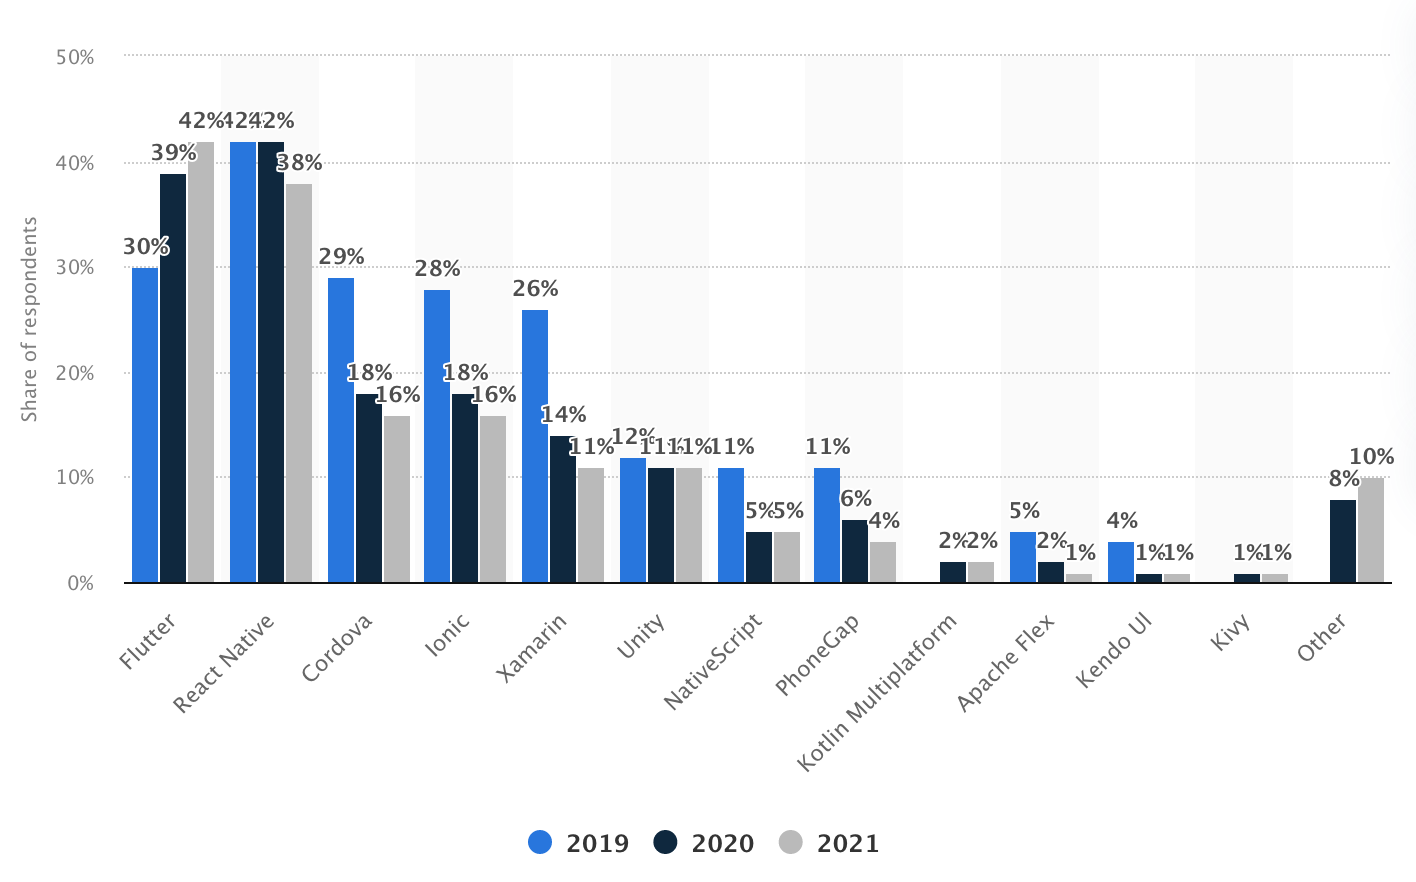
\includegraphics[width=0.85\textwidth]{b_chapters/chapter1/assets/f-1.png}
  \figsource{Author-created illustration based on industry timeline analysis.}
  \caption{Evolution of mobile application development frameworks (2008--2025).}
  \label{fig:mobile-evolution}
\end{figure}

\textbf{Phase~1: Native dominance (2008--2012).}
The first phase was dominated by native development approaches.
Developers created separate codebases for iOS using Objective-C and for Android using Java.
This approach required specialized expertise for each platform and resulted in high development costs, as essentially two complete applications needed to be built and maintained.
The advantages of native development included optimal performance and full access to platform-specific features, but the resource requirements limited this approach to well-funded organizations~\cite{charland2011}.

\textbf{Phase~2: Hybrid emergence (2012--2016).}
The second phase witnessed the emergence of hybrid frameworks designed to address the cost and complexity challenges of native development.
Technologies such as Apache Cordova (PhoneGap) allowed developers to write applications using web technologies (HTML, CSS, JavaScript) and package them for multiple platforms.
Ionic Framework built upon Cordova to provide pre-built UI components.
React Native, released by Facebook in 2015, introduced a different approach using native components rather than web views~\cite{biorn2017}.
These technologies promised write-once-deploy-everywhere capability but often suffered from performance limitations and inconsistent user experiences~\cite{lim2015}.

\textbf{Phase~3: Near-native cross-platform (2017--present).}
The current phase is characterized by sophisticated cross-platform frameworks achieving near-native performance while maintaining the single-codebase advantage.
Flutter, released by Google in May 2017 and reaching stable version~1.0 in December 2018, represents a significant advancement.
Unlike predecessors, Flutter compiles to native ARM code and renders its own widgets using the Skia graphics engine, achieving consistent visual appearance and 60~fps animations on standard devices~\cite{flutter_arch2024}.

The global mobile application market has demonstrated consistent growth throughout this evolution.
According to Statista, mobile app downloads worldwide reached 255~billion in 2022, with revenue exceeding 430~billion~USD~\cite{statista2024}.
In Uzbekistan, internet penetration reached approximately 77\% in 2023, with mobile devices accounting for the majority of internet access.
The success of local mobile payment applications such as Click and Payme demonstrates that Uzbek consumers are ready to adopt mobile solutions that provide genuine value~\cite{gartner2023}.


% =====================================================================
\section{Analysis of Online Booking Systems}
\label{sec:booking-analysis}

The restaurant booking industry has evolved from simple telephone reservation systems to sophisticated platforms offering comprehensive hospitality solutions.
Understanding existing platforms provides valuable context for the development of CHOYXONA.UZ and helps identify both successful patterns and gaps that remain unaddressed in certain markets.

\textbf{OpenTable}, founded in 1998, pioneered online restaurant reservations and remains one of the largest platforms globally.
Acquired by Booking Holdings in 2014 for approximately 2.6~billion~USD, OpenTable serves over 60,000 restaurants with a comprehensive reservation management system including floor management, guest profiles, analytics dashboards, and POS integration.
Revenue comes from monthly subscription fees and per-cover charges~\cite{opentable2023}.

\textbf{TheFork}, a TripAdvisor company, demonstrates the importance of integration with review ecosystems.
By combining reservation functionality with millions of TripAdvisor reviews, TheFork provides discovery-to-booking experiences primarily in European markets.
Its \enquote{Yums} loyalty program incentivizes repeat bookings~\cite{gartner2023}.

\textbf{Resy}, founded in 2014 and acquired by American Express in 2019, targets the high-end dining segment with exclusive access to sought-after reservations.
Integration with American Express card benefits provides priority access, highlighting natural synergies between dining reservations and payment ecosystems.

\textbf{Yelp Reservations} demonstrates how discovery platforms naturally extend into transactional functionality.
Yelp's strength in user-generated reviews and local search makes it significant in the restaurant discovery journey, even when actual booking transactions occur through partner services~\cite{nielsen2012}.

A comparative analysis of these platforms reveals several common success factors, summarized in \cref{tab:platform-comparison}.

\begin{table}[htbp]
\caption{Comparison of global restaurant booking platforms}
\label{tab:platform-comparison}
\centering
\small
\begin{tabular}{lcccc}
\toprule
\textbf{Feature} & \textbf{OpenTable} & \textbf{TheFork} & \textbf{Resy} & \textbf{Yelp} \\
\midrule
Two-sided marketplace  & \checkmark & \checkmark & \checkmark & \checkmark \\
Review \& rating system & \checkmark & \checkmark & Partial    & \checkmark \\
Loyalty program         & ---        & \checkmark & \checkmark & ---        \\
POS integration         & \checkmark & Partial    & \checkmark & ---        \\
Mobile app              & \checkmark & \checkmark & \checkmark & \checkmark \\
Private room booking    & Partial    & ---        & ---        & ---        \\
Central Asian coverage  & ---        & ---        & ---        & ---        \\
Multilingual (UZ/RU/EN) & ---        & ---        & ---        & ---        \\
\bottomrule
\end{tabular}
\end{table}

As \cref{tab:platform-comparison} demonstrates, none of the major platforms provide Central Asian market coverage or support for Uzbek and Russian languages.
Furthermore, the private room booking capability essential for choyxona culture is either absent or only partially supported.
The Central Asian market presents unique characteristics that differentiate it from Western markets: teahouses feature private rooms for extended gatherings lasting several hours, cultural preferences regarding hospitality create specific requirements, and menu offerings center around traditional cuisine with specific preparation requirements~\cite{gartner2023}.

\begin{figure}[htbp]
  \centering
  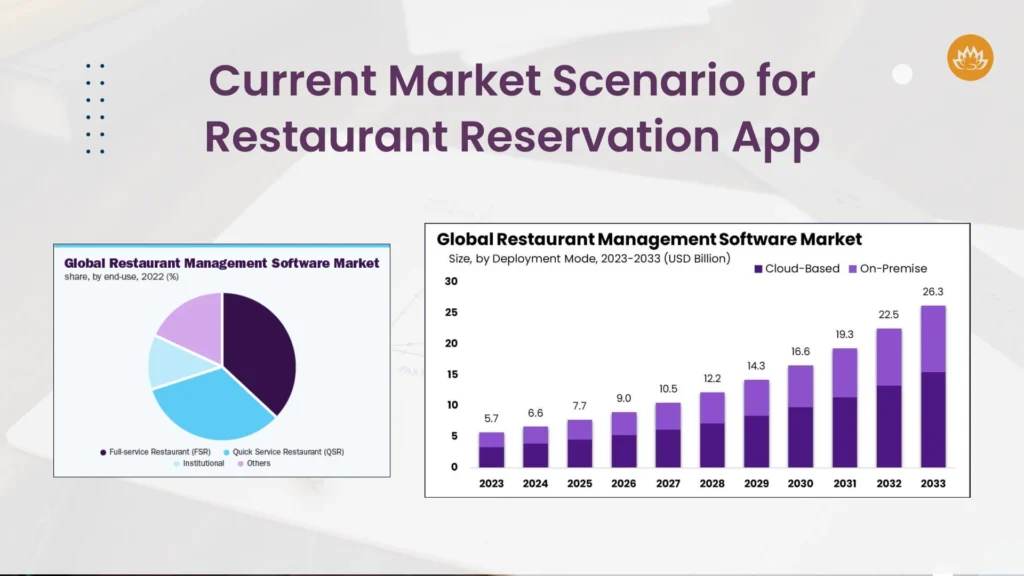
\includegraphics[width=0.7\textwidth]{b_chapters/chapter1/assets/f-2.png}
  \figsource{Author-created illustration based on platform analysis.}
  \caption{Feature coverage analysis of global booking platforms vs. Uzbek market requirements.}
  \label{fig:platform-gap}
\end{figure}

The competitive landscape in Uzbekistan for restaurant booking is currently limited.
While general business directories and social media pages provide some discovery functionality, no dedicated booking platform with real-time availability and confirmation has achieved significant adoption.
This gap validates the opportunity for CHOYXONA.UZ to establish market leadership with a culturally adapted solution.


% =====================================================================
\section{Flutter Framework: Architecture and Advantages}
\label{sec:flutter}

Flutter is an open-source user interface software development kit created by Google that enables developers to build natively compiled applications for mobile, web, and desktop platforms from a single codebase written in the Dart programming language.
Since its initial stable release in December 2018, Flutter has grown rapidly, with Google reporting over 3~million developers using the framework by 2022~\cite{flutter_arch2024}.

The architecture of Flutter differs fundamentally from other cross-platform solutions, as illustrated in \cref{fig:flutter-arch}.
While frameworks like React Native bridge JavaScript code to native components through a middleware layer, Flutter maintains its own rendering engine based on Skia --- the same graphics library used by Google Chrome and Android.
Rather than wrapping or bridging to platform-specific components, Flutter draws every pixel of the user interface directly using its own rendering pipeline~\cite{windmill2020}.

\begin{figure}[htbp]
  \centering
  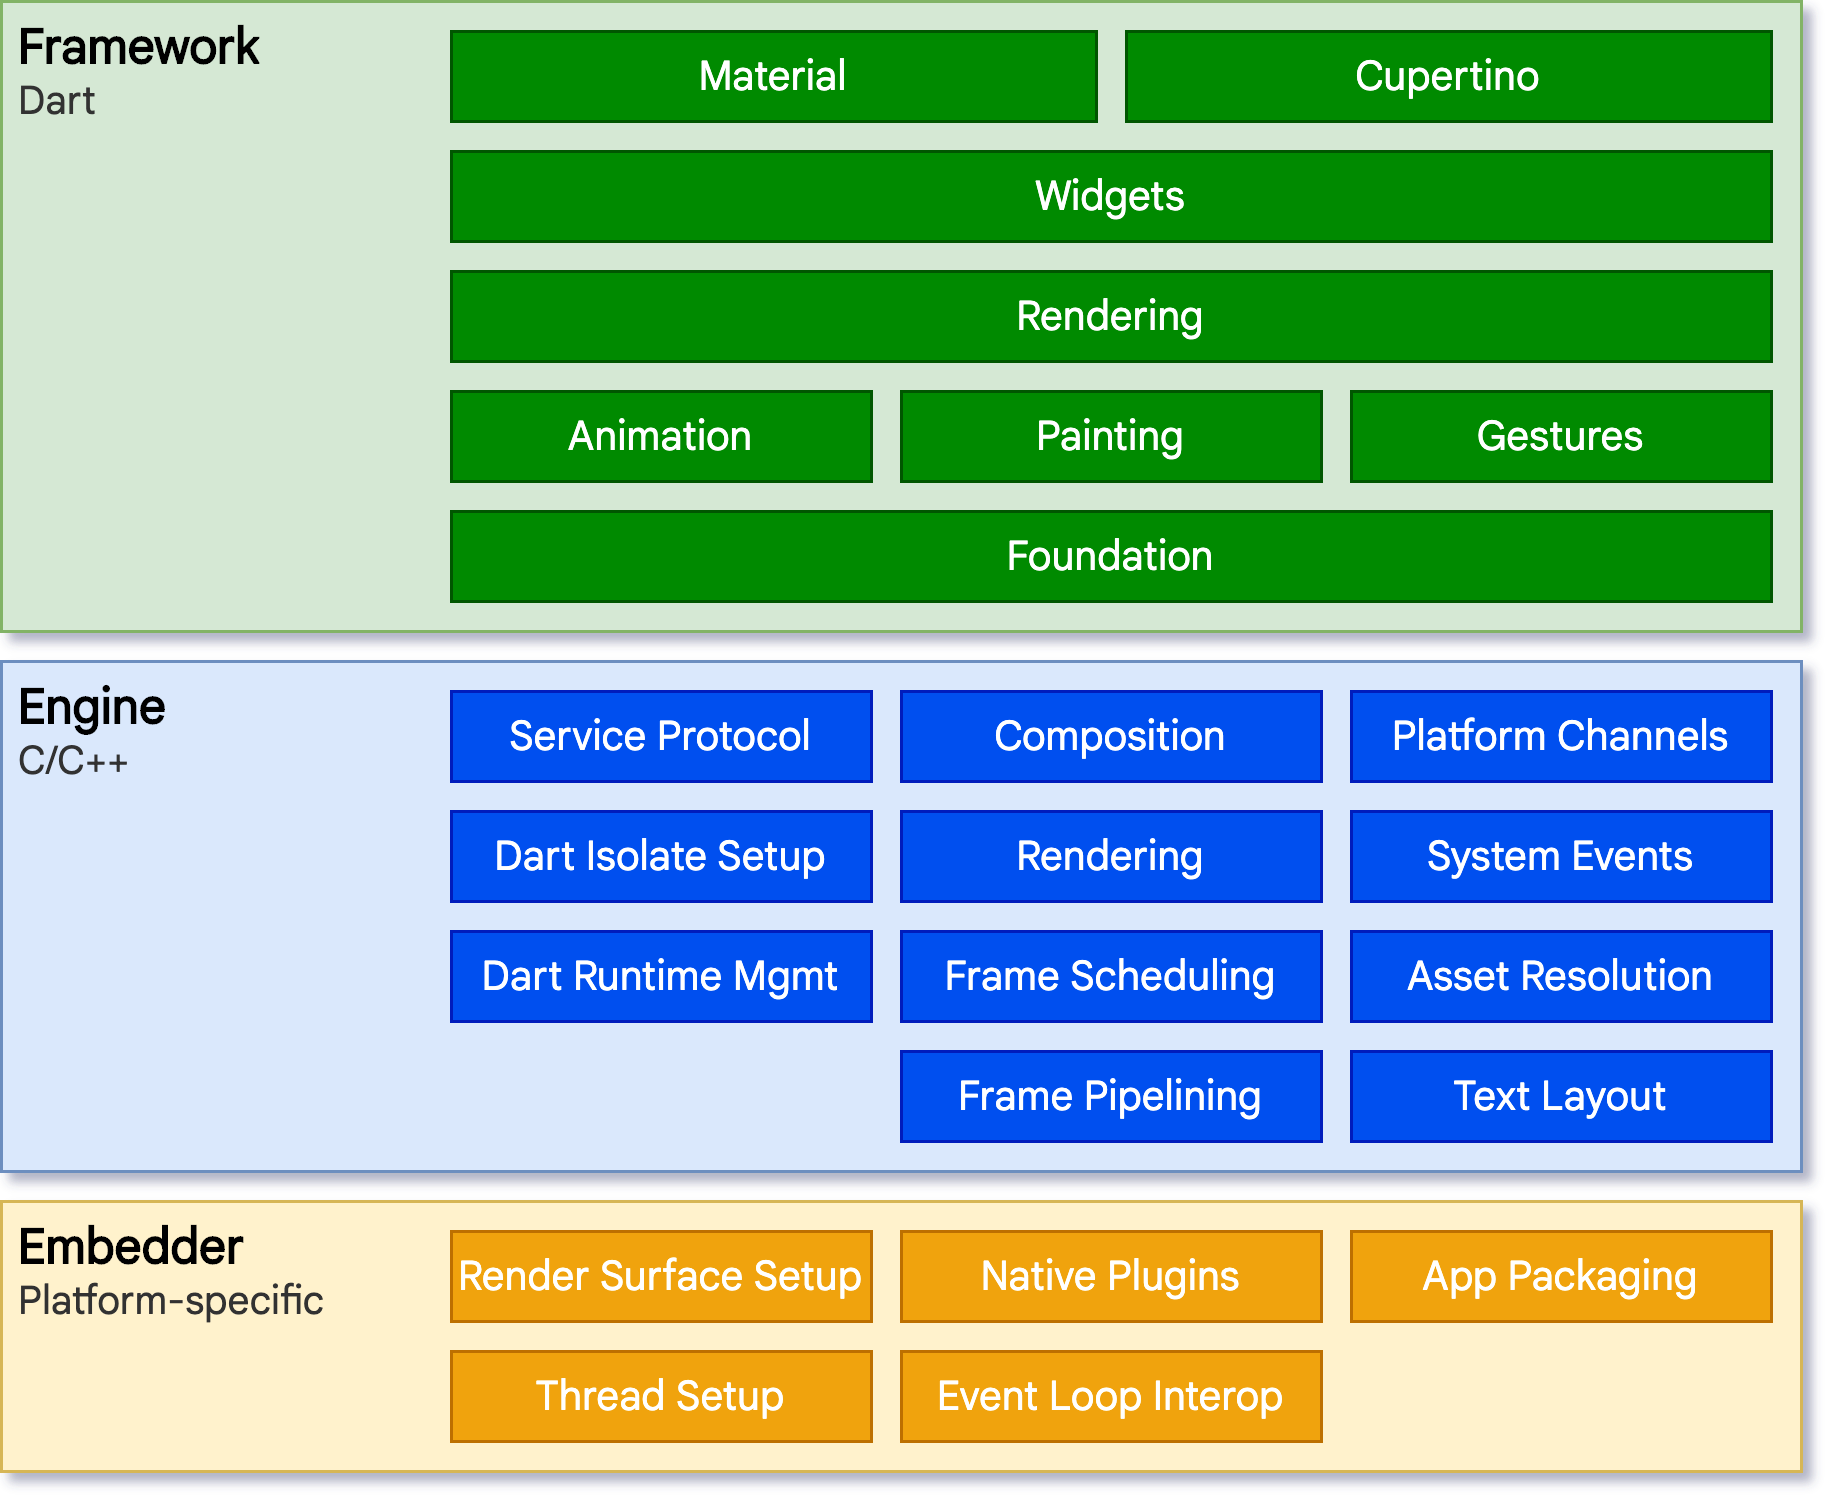
\includegraphics[width=0.75\textwidth]{b_chapters/chapter1/assets/f-3.png}
  \figsource{Adapted from Flutter official documentation~\cite{flutter_arch2024}.}
  \caption{Flutter framework architecture and rendering pipeline.}
  \label{fig:flutter-arch}
\end{figure}

This architecture provides several significant advantages:
\begin{itemize}
  \item \textbf{Visual consistency} across platforms, since the same rendering code executes on both iOS and Android.
  \item \textbf{Fine-grained pixel control}, enabling precise implementation of custom designs.
  \item \textbf{High-performance animations} at 60~fps on standard devices and 120~fps on high-refresh-rate displays.
  \item \textbf{Hot reload} capability reflecting code changes within milliseconds during development, transforming the iteration experience~\cite{napoli2021}.
\end{itemize}

The \textbf{Dart programming language}, created by Google, provides features well-suited for UI programming: compilation to native ARM code for performance, both ahead-of-time and just-in-time compilation, strong static typing with type inference, null safety (since Dart~2.12), and asynchronous programming support through futures and streams~\cite{dart2024}.

Flutter's \textbf{widget-based architecture} organizes the user interface as a tree of immutable widget objects.
Everything in Flutter is a widget --- from structural elements like rows and columns to interactive elements like buttons and text fields.
When application state changes, Flutter rebuilds the affected portion of the widget tree and efficiently updates only the changed portions of the rendering tree.
This declarative approach simplifies UI development and reduces bugs associated with manually managing view updates~\cite{payne2019}.

\textbf{State management} represents a critical architectural decision.
The Provider package, officially recommended by the Flutter team, implements the InheritedWidget pattern for efficient state sharing.
Alternative approaches include BLoC (Business Logic Component) using streams, Riverpod with improved error handling, and GetX prioritizing developer convenience~\cite{flutter_state2024}.
CHOYXONA.UZ employs Provider for state management, balancing simplicity with sufficient capability.

A comparative analysis of cross-platform frameworks informed the technology selection, as summarized in \cref{tab:framework-comparison}.

\begin{table}[htbp]
\caption{Comparison of cross-platform mobile development frameworks}
\label{tab:framework-comparison}
\centering
\small
\begin{tabular}{lccc}
\toprule
\textbf{Criterion} & \textbf{Flutter} & \textbf{React Native} & \textbf{Kotlin MP} \\
\midrule
Language              & Dart         & JavaScript/TS   & Kotlin       \\
Rendering             & Own engine   & Native bridge   & Native UI    \\
Performance           & Near-native  & Good            & Native       \\
UI consistency        & Excellent    & Platform-dependent & Platform-native \\
Hot reload            & \checkmark   & \checkmark      & Partial      \\
Single codebase       & \checkmark   & \checkmark      & Logic only   \\
Community size        & Large        & Very large      & Growing      \\
Desktop/Web support   & \checkmark   & Limited         & Experimental \\
Google backing        & \checkmark   & Meta            & JetBrains    \\
Null safety           & \checkmark   & TypeScript      & \checkmark   \\
\bottomrule
\end{tabular}
\end{table}

Flutter was selected for CHOYXONA.UZ based on alignment with project requirements: the single codebase approach matched resource constraints, the modern Dart language reduces runtime errors, the extensive widget library provides pre-built Material Design components, and Google's continued investment ensures long-term viability~\cite{wu2018, xanthopoulos2013}.


% =====================================================================
\section{Firebase Backend-as-a-Service}
\label{sec:firebase}

Firebase is a comprehensive application development platform provided by Google, offering a suite of services that accelerate development by handling common backend requirements.
Originally founded as an independent company in 2011 focused on real-time database functionality, Firebase was acquired by Google in 2014 and has expanded to include authentication, hosting, cloud functions, analytics, and numerous other services~\cite{moroney2017}.
The Firebase services architecture relevant to CHOYXONA.UZ is presented in \cref{fig:firebase-services}.

\begin{figure}[htbp]
  \centering
  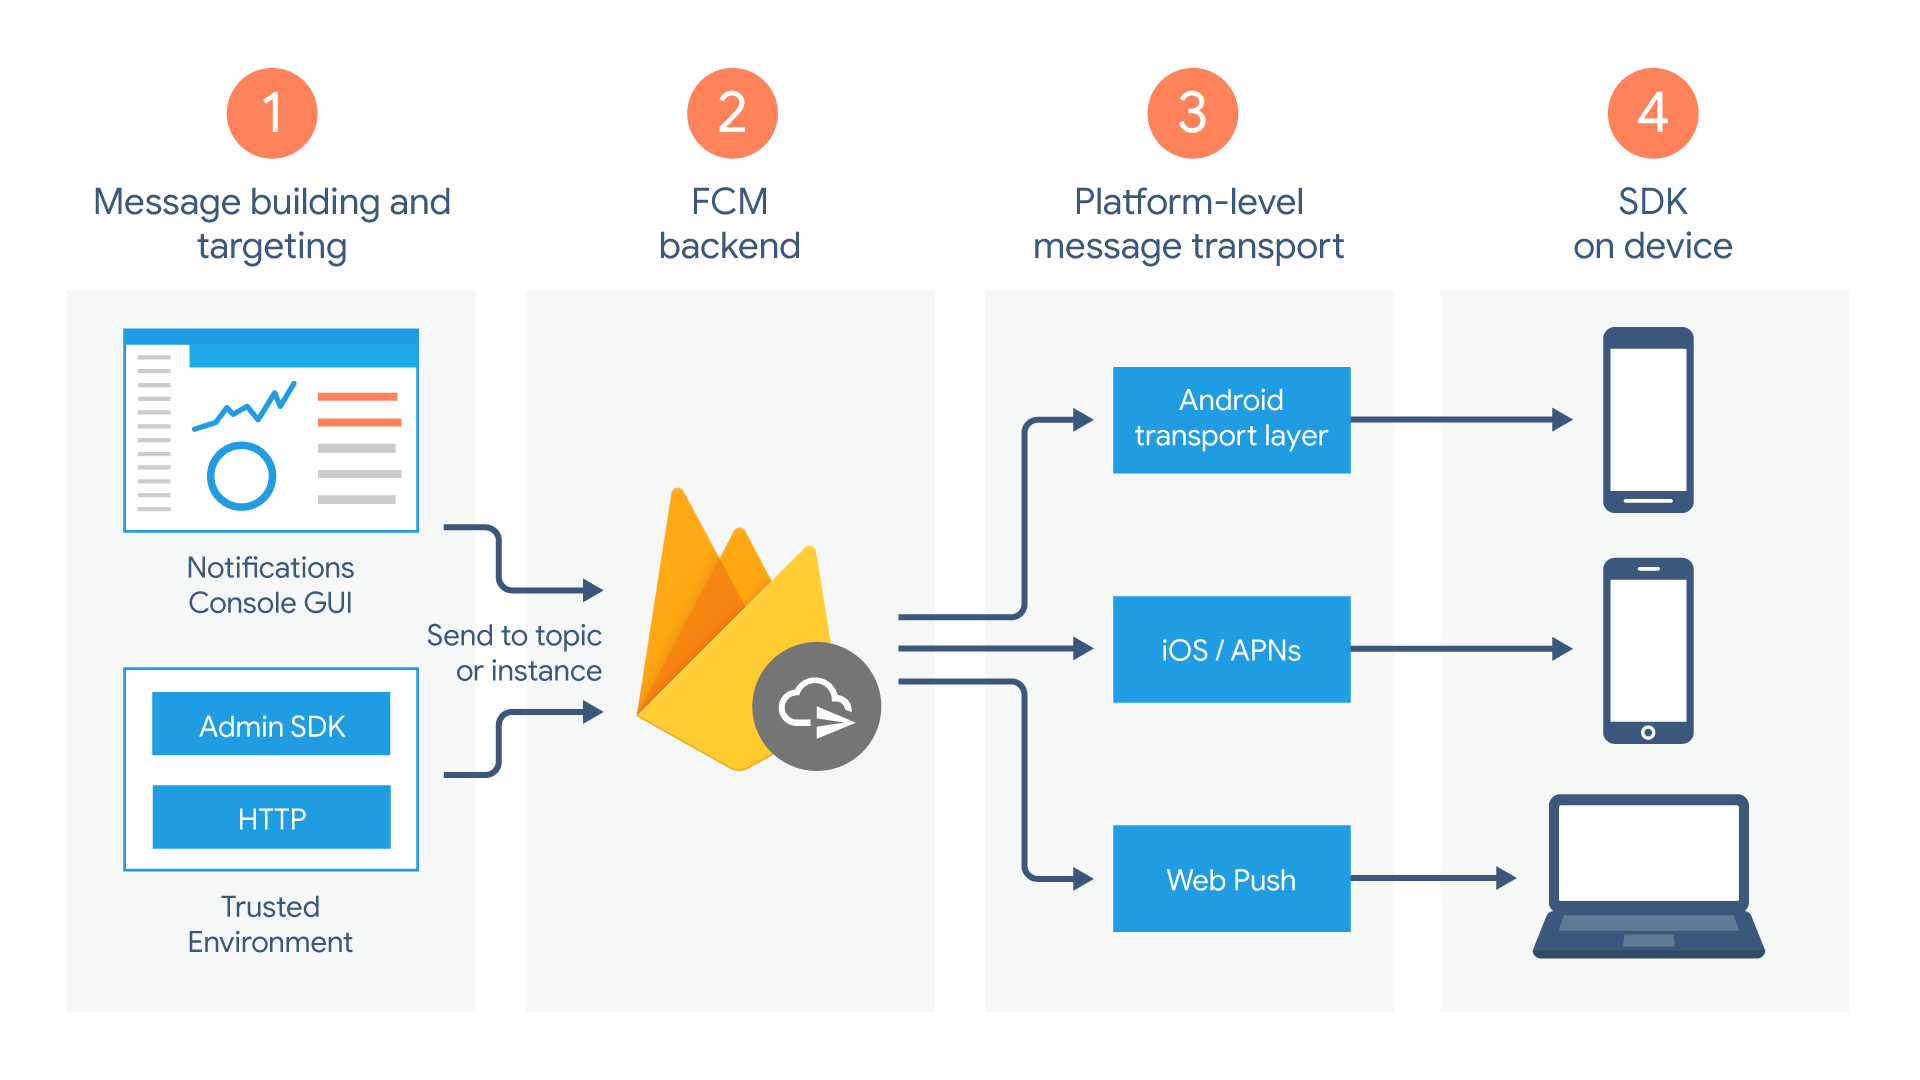
\includegraphics[width=0.75\textwidth]{b_chapters/chapter1/assets/f-4.png}
  \figsource{Author-created illustration based on Firebase documentation~\cite{firebase_auth2024}.}
  \caption{Firebase services architecture used in the CHOYXONA.UZ application.}
  \label{fig:firebase-services}
\end{figure}

\textbf{Firebase Authentication} supports multiple sign-in methods.
For CHOYXONA.UZ, email/password and phone number (SMS) authentication were implemented, aligning with user expectations in Uzbekistan where phone numbers serve as primary identifiers.
The service handles secure password hashing, session management, brute-force protection, and account recovery~\cite{firebase_auth2024}.

\textbf{Cloud Firestore} serves as the primary database, providing flexible, scalable NoSQL document storage with real-time synchronization capabilities.
Unlike traditional SQL databases with fixed schemas, Firestore stores data in collections of documents containing key-value pairs and subcollections for hierarchical organization.
The real-time synchronization capability enables Firestore clients to subscribe to document snapshots, receiving automatic updates through persistent connections whenever data changes on the server~\cite{firebase_firestore2024}.
This capability is particularly valuable for booking applications where availability can change rapidly.

\textbf{Firebase Cloud Storage} provides secure file storage for user-generated content including profile photos, establishment images, and menu item photos.
Storage security rules reference the authenticated user's identity, enabling patterns such as allowing users to upload their own profile photos while preventing modification of others' files~\cite{moroney2017}.

\textbf{Firebase Cloud Messaging (FCM)} enables push notifications on both Android and iOS platforms.
CHOYXONA.UZ uses FCM for booking confirmations, reservation reminders (24~hours and 2~hours before), promotional notifications from establishments, and system announcements.
The notification system reaches users even when the application is not actively running~\cite{firebase_functions2024}.

The \textbf{pricing model} follows a usage-based approach with generous free tiers.
The free Spark plan includes 1~GiB Firestore storage, 10~GiB Cloud Storage, and 50,000 daily active users for Authentication.
The Blaze plan charges based on actual usage, reducing initial infrastructure investment while providing a clear scaling path~\cite{khawas2018}.

\textbf{Security Rules} enforce authorization declaratively at the database level.
Rules execute on Firebase servers, ensuring enforcement regardless of client behavior.
CHOYXONA.UZ implements role-based access control: regular users can only read their own bookings, administrators manage their own establishment, and super administrators have broader platform access~\cite{firebase_firestore2024}.

The integration of Firebase services into the Flutter application leverages official packages maintained by the \textbf{FlutterFire} project: \texttt{firebase\_core} for initialization, \texttt{firebase\_auth} for authentication, \texttt{cloud\_firestore} for database access, \texttt{firebase\_storage} for file management, and \texttt{firebase\_messaging} for push notifications~\cite{firebase_auth2024}.


% =====================================================================
\section{Research Motivation and Direction}
\label{sec:motivation}

\textbf{Problem significance.}
The analysis conducted in \cref{sec:booking-analysis} reveals that the Central Asian hospitality market remains unserved by major international booking platforms.
Uzbekistan, with over 35~million population and rapidly growing smartphone penetration, represents a significant addressable market.
Customers face difficulty discovering establishments matching their preferences, uncertainty about availability, and limited access to reviews.
Establishment owners lack tools for efficient booking management, customer analytics, and digital marketing~\cite{gartner2023}.

\textbf{Identified gap.}
From the comparison in \cref{sec:booking-analysis} and \cref{tab:platform-comparison}, the unmet need is clear: no existing platform provides a localized, culturally adapted booking solution that supports Uzbek teahouse conventions (private rooms, extended gatherings), multilingual interface (Uzbek, Russian, English), and real-time availability management tailored to the regional market.

\textbf{Direction and scope.}
This thesis pursues the development of CHOYXONA.UZ --- a complete cross-platform mobile application addressing the identified gap.
The scope encompasses:
\begin{itemize}
  \item Customer-facing features for discovery, search, and booking.
  \item Administrator tools for establishment management and analytics.
  \item Super administrator capabilities for platform oversight.
  \item Multi-platform deployment strategy for maximum market reach.
\end{itemize}
Deliberately out of scope for the initial release: integrated payment processing, AI-powered recommendations, and geographic expansion beyond Uzbekistan.

\textbf{Success criteria.}
The approach succeeds if: (1)~the application achieves acceptable performance metrics (cold start under 3~seconds, 60~fps scrolling, sub-200~ms query latency); (2)~successful deployment to Google Play, App Store, and alternative marketplaces; (3)~positive user acceptance testing results validating usability across target personas.


% =====================================================================
\section{Chapter Summary}
\label{sec:ch1-summary}

This chapter established the theoretical and analytical foundation for the CHOYXONA.UZ project through four key contributions:

First, \cref{sec:core-concepts} defined the conceptual vocabulary including cross-platform development, BaaS, real-time synchronization, and the choyxona cultural context that governs application requirements.

Second, \cref{sec:mobile-evolution} traced the evolution of mobile development through three phases --- native dominance, hybrid emergence, and near-native cross-platform --- demonstrating that modern frameworks like Flutter have matured to a point where single-codebase development no longer requires significant performance or quality compromises.

Third, \cref{sec:booking-analysis} conducted a comparative analysis of major booking platforms (OpenTable, TheFork, Resy, Yelp), identifying that while these platforms successfully serve Western markets, none provide coverage for Central Asia, support for Uzbek/Russian languages, or accommodation of choyxona-specific booking patterns such as private room reservations.

Fourth, \cref{sec:flutter,sec:firebase} justified the technology selection of Flutter and Firebase through systematic comparison with alternatives (\cref{tab:framework-comparison}), demonstrating alignment with project constraints including small team size, cross-platform requirements, real-time data needs, and cost-effective infrastructure.

Finally, \cref{sec:motivation} articulated the concrete research gap --- the absence of a localized, culturally adapted booking platform for Uzbekistan --- and defined measurable success criteria that will be evaluated in \cref{ch:testing}.

These analyses motivate the system architecture and design presented in Chapter~2 and the implementation described in Chapter~3.

\chapter{System Architecture and Technical Design}
\label{ch:architecture}

This chapter presents the system architecture and technical design decisions of the CHOYXONA.UZ application.
It covers the overall architectural approach, database structure and data modeling in Cloud Firestore, user interface design principles with responsive layout strategy, real-time data synchronization mechanisms, and Google Maps integration for geolocation services.


% =====================================================================
\section{General System Architecture}
\label{sec:system-arch}

The architecture of CHOYXONA.UZ follows a client-server model with Firebase services providing the complete backend infrastructure.
This architectural approach eliminates the need for deploying and maintaining custom server software, allowing development resources to focus on the user-facing application while leveraging Google's infrastructure for reliability, scalability, and global availability~\cite{moroney2017}.

The system architecture consists of three primary layers working together to deliver the application functionality:

\begin{enumerate}
  \item \textbf{Presentation layer} --- implemented entirely in Flutter, this layer handles all user interface rendering, user interaction, and navigation logic that creates the visual experience users interact with.
  \item \textbf{Business logic layer} --- combines client-side Dart code executing within the Flutter application with Firebase Cloud Functions executing on Google's servers for operations requiring elevated privileges or triggered by database events.
  \item \textbf{Data layer} --- managed by Cloud Firestore for structured data and Cloud Storage for binary files (images, documents), this layer persists all application state and user-generated content.
\end{enumerate}

Client applications communicate with Firebase services through official SDKs that handle authentication, network connectivity, data serialization, and local caching.
The Firebase SDK manages network connections automatically, retrying failed requests with exponential backoff and queuing write operations when offline for later synchronization~\cite{firebase_firestore2024}.
This automatic handling of network unreliability significantly reduces application code complexity while improving user experience in conditions with intermittent connectivity --- a particularly relevant consideration in Uzbekistan where mobile network quality varies by region.

The Flutter application organizes code following a \textbf{feature-based structure} that groups related files by functionality rather than by technical type.
The main source directories include:

\begin{itemize}
  \item \texttt{models/} --- Dart classes representing business entities (users, establishments, bookings);
  \item \texttt{services/} --- classes encapsulating Firebase interactions and backend communication;
  \item \texttt{screens/} --- UI components organized by feature area (authentication, home, search, booking, profile);
  \item \texttt{widgets/} --- reusable UI components used across multiple screens;
  \item \texttt{core/} --- shared utilities including theme definitions, constants, and helper functions.
\end{itemize}

This organization follows the separation of concerns principle recommended by Martin~\cite{martin2017}, enabling clear code boundaries while keeping related files together for easier navigation and maintenance.

The high-level interaction between system components is illustrated in \cref{fig:system-arch}.

\begin{figure}[htbp]
  \centering
  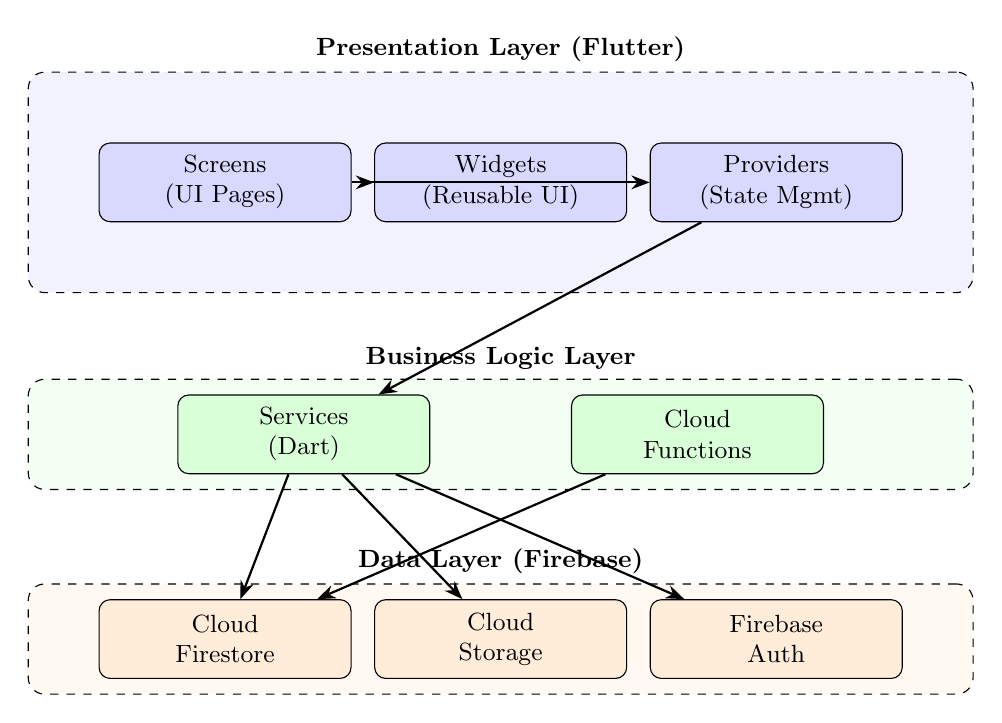
\begin{tikzpicture}[
    box/.style={draw, rounded corners=4pt, minimum width=3.2cm, minimum height=1cm, align=center, font=\small},
    layer/.style={draw, dashed, rounded corners=6pt, inner sep=8pt, fill=#1!5},
    arr/.style={->, thick, >=Stealth},
    node distance=1cm and 1.5cm
  ]
    % Presentation Layer
    \node[layer=blue, minimum width=12cm, minimum height=2.8cm, label={[font=\small\bfseries]above:Presentation Layer (Flutter)}] (pl) {};
    \node[box, fill=blue!15] at (-3.5,0) (screens) {Screens\\(UI Pages)};
    \node[box, fill=blue!15] at (0,0) (widgets) {Widgets\\(Reusable UI)};
    \node[box, fill=blue!15] at (3.5,0) (providers) {Providers\\(State Mgmt)};
    \draw[arr] (screens) -- (widgets);
    \draw[arr] (screens) -- (providers);

    % Business Logic Layer  
    \node[layer=green, minimum width=12cm, minimum height=1.4cm, label={[font=\small\bfseries]above:Business Logic Layer}] (bl) at (0,-3.2) {};
    \node[box, fill=green!15] at (-2.5,-3.2) (services) {Services\\(Dart)};
    \node[box, fill=green!15] at (2.5,-3.2) (functions) {Cloud\\Functions};

    % Data Layer
    \node[layer=orange, minimum width=12cm, minimum height=1.4cm, label={[font=\small\bfseries]above:Data Layer (Firebase)}] (dl) at (0,-5.8) {};
    \node[box, fill=orange!15] at (-3.5,-5.8) (firestore) {Cloud\\Firestore};
    \node[box, fill=orange!15] at (0,-5.8) (storage) {Cloud\\Storage};
    \node[box, fill=orange!15] at (3.5,-5.8) (auth) {Firebase\\Auth};

    % Arrows
    \draw[arr] (providers) -- (services);
    \draw[arr] (services) -- (firestore);
    \draw[arr] (services) -- (storage);
    \draw[arr] (services) -- (auth);
    \draw[arr] (functions) -- (firestore);
  \end{tikzpicture}
  \caption{High-level system architecture of CHOYXONA.UZ showing three-layer organization.}
  \label{fig:system-arch}
\end{figure}

The three-layer architecture ensures that changes to one layer have minimal impact on others.
For example, switching from Cloud Firestore to a different database would require changes only in the services layer, leaving the presentation layer and its associated state management intact.
Similarly, UI redesign affects only the presentation layer without requiring modifications to business logic or data access code.


% =====================================================================
\section{Database Design and Data Model}
\label{sec:database}

The database design in Cloud Firestore utilizes several collections to store application data, with each collection containing documents that represent individual entities.
Firestore's NoSQL document model provides flexibility for varying data shapes without requiring schema migrations~\cite{firebase_firestore2024}.

\subsection{Primary Collections}
\label{subsec:collections}

The \textbf{users} collection contains a document for each registered user, identified by their Firebase Authentication UID.
User documents store:
\begin{itemize}
  \item Profile information: \texttt{displayName}, \texttt{email}, \texttt{phoneNumber}, \texttt{photoURL};
  \item Role assignment: possible values including \texttt{user}, \texttt{admin}, and \texttt{superadmin};
  \item Associated establishment identifier (for administrator accounts);
  \item User preferences: language selection and notification settings;
  \item Account status and creation timestamp.
\end{itemize}

The \textbf{choyxonas} collection holds establishment data with each document representing one restaurant or teahouse.
Establishment documents contain essential information including name, description, and establishment type categorized as traditional teahouse, national cuisine, European cuisine, or mixed menu.
Location data includes address text, region identifier for filtering, and geographic coordinates stored as a \texttt{GeoPoint} for map display and distance calculations.
Contact information encompasses phone numbers, social media links, and website URL.
Operating schedule stores hours for each day of the week.
Amenities list features such as Wi-Fi, parking, and private rooms using a string array.

The \textbf{bookings} collection tracks reservations with documents linking users to establishments at specific times.
Booking documents contain references to the user and establishment documents, enabling queries from either direction.
Temporal data includes the booking date, start time, and expected duration.
The status field tracks the booking lifecycle through states: \textit{pending} $\to$ \textit{confirmed} $\to$ \textit{completed} (or \textit{cancelled}/\textit{no-show}).
This lifecycle is visualized in \cref{fig:booking-lifecycle}.

\begin{figure}[htbp]
  \centering
  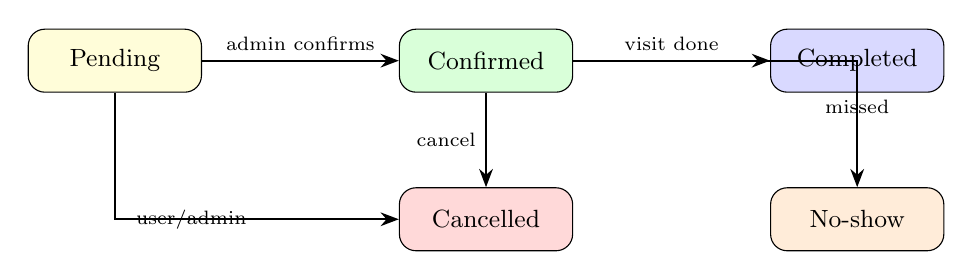
\begin{tikzpicture}[
    state/.style={draw, rounded corners=6pt, minimum width=2.2cm, minimum height=0.8cm, align=center, font=\small, fill=#1!15},
    arr/.style={->, thick, >=Stealth},
    node distance=2.5cm
  ]
    \node[state=yellow] (pending)   {Pending};
    \node[state=green,  right=of pending]   (confirmed) {Confirmed};
    \node[state=blue,   right=of confirmed] (completed) {Completed};
    \node[state=red,    below=1.2cm of confirmed] (cancelled) {Cancelled};
    \node[state=orange, right=of cancelled] (noshow)    {No-show};

    \draw[arr] (pending)   -- node[above,font=\scriptsize]{admin confirms} (confirmed);
    \draw[arr] (confirmed) -- node[above,font=\scriptsize]{visit done} (completed);
    \draw[arr] (pending)   |- node[near end,left,font=\scriptsize]{user/admin} (cancelled);
    \draw[arr] (confirmed) -- node[left,font=\scriptsize]{cancel} (cancelled);
    \draw[arr] (confirmed) -| node[near end,above,font=\scriptsize]{missed} (noshow);
  \end{tikzpicture}
  \caption{Booking status lifecycle showing state transitions from creation to completion.}
  \label{fig:booking-lifecycle}
\end{figure}

Additional collections support auxiliary features:
\begin{itemize}
  \item \textbf{reviews} --- user ratings and text feedback with references to user and establishment;
  \item \textbf{orders} --- in-venue ordering tracking menu items, quantities, and order status;
  \item \textbf{notifications} --- push notification history for each user;
  \item \textbf{promotions} --- marketing campaigns and special offers from establishments.
\end{itemize}


\subsection{Data Modeling Strategies}
\label{subsec:data-modeling}

Document structure was designed to optimize common query patterns while minimizing data redundancy and read costs.
\textbf{Denormalization} is employed strategically where read performance justifies data duplication.
For example, booking documents embed the establishment name rather than only storing a reference, avoiding an additional Firestore read when displaying booking history.
The tradeoff is that establishment name changes require updating associated bookings, handled through batch operations~\cite{firebase_firestore2024}.

\textbf{Subcollections} organize hierarchical data: menu items exist as a subcollection under each establishment document rather than as a top-level collection, ensuring menu queries are naturally scoped to a single establishment.
This also means that loading establishment list data does not inadvertently load all menu items as well.

The entity-relationship structure of the primary data model is shown in \cref{tab:er-model}.

\begin{table}[htbp]
\caption{Entity-relationship summary of the CHOYXONA.UZ data model}
\label{tab:er-model}
\centering
\small
\begin{tabular}{llll}
\toprule
\textbf{Entity (Collection)} & \textbf{Key Fields} & \textbf{Relationships} & \textbf{Subcollections} \\
\midrule
\texttt{users}      & name, email, role, phone & $\to$ choyxonas (admin) & favorites \\
\texttt{choyxonas}  & name, location, type, status & $\to$ users (admin ref) & menu, rooms \\
\texttt{bookings}   & date, time, status, guests & $\to$ users, choyxonas & --- \\
\texttt{reviews}    & rating, text, timestamp & $\to$ users, choyxonas & --- \\
\texttt{notifications} & title, body, read status & $\to$ users & --- \\
\bottomrule
\end{tabular}
\end{table}


\subsection{Indexing and Security}
\label{subsec:indexing-security}

\textbf{Indexing strategy} considers the filtering, sorting, and pagination operations required by the application.
Firestore automatically creates indexes for single-field queries, but composite indexes must be explicitly defined for multi-field queries.
The \texttt{firestore.indexes.json} configuration file defines composite indexes supporting common queries such as:
\begin{itemize}
  \item Filtering establishments by region while sorting by rating;
  \item Querying bookings for an establishment ordered by date;
  \item Filtering reviews by establishment while sorting by recency.
\end{itemize}

\textbf{Security rules} implement role-based access control at the database level.
Rules execute on Firebase servers, ensuring enforcement regardless of client behavior~\cite{firebase_firestore2024}.
The access control matrix is summarized in \cref{tab:security-rules}.

\begin{table}[htbp]
\caption{Firestore security rules --- access control matrix by user role}
\label{tab:security-rules}
\centering
\small
\begin{tabular}{lcccc}
\toprule
\textbf{Collection} & \textbf{Operation} & \textbf{User} & \textbf{Admin} & \textbf{Super Admin} \\
\midrule
users      & Read own    & \checkmark & \checkmark & \checkmark \\
users      & Write own   & \checkmark & \checkmark & \checkmark \\
users      & Read others & ---        & ---        & \checkmark \\
choyxonas  & Read        & \checkmark & \checkmark & \checkmark \\
choyxonas  & Write own   & ---        & \checkmark & \checkmark \\
bookings   & Create      & \checkmark & ---        & --- \\
bookings   & Read own    & \checkmark & \checkmark$^*$ & \checkmark \\
bookings   & Update status & ---      & \checkmark$^*$ & \checkmark \\
reviews    & Create      & \checkmark & ---        & --- \\
reviews    & Read        & \checkmark & \checkmark & \checkmark \\
\bottomrule
\multicolumn{5}{l}{\scriptsize $^*$ Admin access limited to their own establishment's data.}
\end{tabular}
\end{table}


% =====================================================================
\section{User Interface Design and Responsive Approach}
\label{sec:ui-design}

The user interface of CHOYXONA.UZ adheres to Material Design~3 guidelines while incorporating elements that resonate with the target cultural context~\cite{material2024}.
The design philosophy prioritizes clarity, accessibility, and efficient task completion across all user journeys.

\subsection{Visual Design System}
\label{subsec:visual-design}

The visual design employs a carefully selected color palette balancing tradition with modernity.
The primary color, a warm earthy brown tone, evokes the aesthetic of traditional teahouses while maintaining sufficient contrast for accessibility.
Both \textbf{light and dark themes} are fully supported, responding to user preference or system settings.

The \texttt{ThemeProvider} implementation uses Flutter's Provider pattern to manage theme state.
At startup, the provider checks stored preference; if none exists, it follows system setting.
Users can explicitly select light, dark, or automatic mode through the settings screen.
Theme changes take effect immediately without restart~\cite{flutter_state2024}.

Typography follows Material Design recommendations with \texttt{Roboto} as the primary typeface for its readability across sizes and weights.
Font scaling respects system accessibility settings, ensuring users who configure larger text see appropriately scaled text without layout breakage~\cite{nielsen2012}.

\subsection{Navigation Architecture}
\label{subsec:navigation}

Navigation implements a \textbf{bottom navigation bar} for five primary destinations:
\begin{enumerate}
  \item \texttt{Home} --- featured establishments and personalized content;
  \item \texttt{Map View} --- geographic discovery with interactive map;
  \item \texttt{Favorites} --- saved establishments for quick access;
  \item \texttt{Orders} --- booking history and management;
  \item \texttt{Profile} --- account and preference management.
\end{enumerate}

Secondary navigation uses stack-based routing through Navigator~2.0 for deeper navigation flows: from Home to establishment details to booking flow, and back.
Within screens, tabs organize related content --- the establishment detail screen uses tabs to separate Overview, Menu, and Reviews sections~\cite{wasserman2010}.

\subsection{Responsive Layout Strategy}
\label{subsec:responsive}

Responsive design ensures appropriate layouts across device sizes from compact phones to large tablets.
Key breakpoints distinguish layout modes as shown in \cref{tab:breakpoints}.

\begin{table}[htbp]
\caption{Responsive layout breakpoints and corresponding design adaptations}
\label{tab:breakpoints}
\centering
\small
\begin{tabular}{lcl}
\toprule
\textbf{Layout} & \textbf{Width (dp)} & \textbf{Adaptation} \\
\midrule
Compact (phone portrait)  & $< 600$     & Single-column, full-width cards \\
Medium (tablet portrait)  & $600$--$840$  & Two-column grid for lists \\
Expanded (tablet landscape) & $> 840$   & Master-detail side-by-side \\
\bottomrule
\end{tabular}
\end{table}

\texttt{MediaQuery} provides device dimensions enabling conditional layout adjustments, while \texttt{LayoutBuilder} provides parent constraints for components that need to adapt to their allocation~\cite{flutter_arch2024}.

\subsection{Localization}
\label{subsec:localization}

Localization extends beyond text translation to encompass all culture-specific aspects.
The \texttt{EasyLocalization} package manages translation files and runtime language switching.
The application supports three languages:
\begin{itemize}
  \item \textbf{Uzbek} --- primary local language;
  \item \textbf{Russian} --- widely understood due to historical context;
  \item \textbf{English} --- for international visitors and expatriates.
\end{itemize}

Date/time formats, currency displays, and number formatting all adjust to locale conventions.
Language preference persists locally using \texttt{SharedPreferences}, loading on subsequent launches.
The initial language defaults to the device's locale if supported, otherwise falling back to Russian~\cite{sommerville2015}.


% =====================================================================
\section{Real-time Synchronization and Data Streaming}
\label{sec:realtime}

Real-time data synchronization represents a cornerstone feature of CHOYXONA.UZ, differentiating it from simple request-response applications and enabling experiences that feel immediately responsive to changing information~\cite{firebase_firestore2024}.

Traditional applications interact with servers through request-response patterns: the client sends a request, the server returns a response, and the client displays the result.
To see updates, users must explicitly refresh.
This pattern creates poor experiences when timeliness matters --- a user viewing available booking times might make decisions based on stale information if another user has just taken a slot.

Firestore provides an alternative through \textbf{real-time listeners}.
Clients establish persistent subscriptions to documents or collections, receiving automatic updates whenever data changes on the server.
Flutter's reactive model integrates naturally through the \texttt{StreamBuilder} widget, which rebuilds its child whenever the stream emits a new value~\cite{flutter_arch2024}.

In CHOYXONA.UZ, real-time synchronization applies to several key scenarios:
\begin{itemize}
  \item \textbf{Availability display}: when customers view establishment slots, changes from other bookings appear immediately.
  \item \textbf{Admin dashboard}: today's bookings stream updates as new reservations arrive.
  \item \textbf{Reviews}: new reviews appear in real-time as submitted.
  \item \textbf{Notifications}: new notifications surface without manual refresh.
\end{itemize}

The \texttt{DataSyncProvider} class implements centralized stream management for data shared across multiple screens.
Rather than creating new subscriptions each time a widget needs data, the provider maintains canonical streams that multiple consumers share.
This reduces Firebase read operations since multiple listeners to a single stream count as one active listener, not multiple~\cite{khawas2018}.

\textbf{Offline persistence}, enabled by default in the Firestore SDK, extends usability when connectivity is unavailable.
The SDK maintains a local cache of recently accessed documents.
When offline, reads return cached data; writes queue locally and synchronize when connectivity resumes.

For booking operations requiring atomicity, \textbf{Firestore transactions} ensure consistent results.
A booking transaction reads current bookings for the requested time, verifies no conflict exists, and creates the new booking atomically.
If another booking was created between the read and write, the transaction retries with fresh data.
\textbf{Optimistic updates} improve perceived responsiveness --- the UI immediately displays a pending booking while the write proceeds asynchronously, reverting only if the write fails~\cite{firebase_firestore2024}.


% =====================================================================
\section{Google Maps Integration and Geolocation Services}
\label{sec:maps}

Geographic functionality significantly enhances discovery and navigation in CHOYXONA.UZ, enabling users to find establishments near their current location, visualize options on a map, and obtain directions~\cite{sommerville2015}.

Integration with Google Maps Platform provides the foundation.
The \texttt{google\_maps\_flutter} package renders interactive maps within the Flutter application as native components, providing smooth gesture-based panning and zooming.

\begin{figure}[htbp]
  \centering
  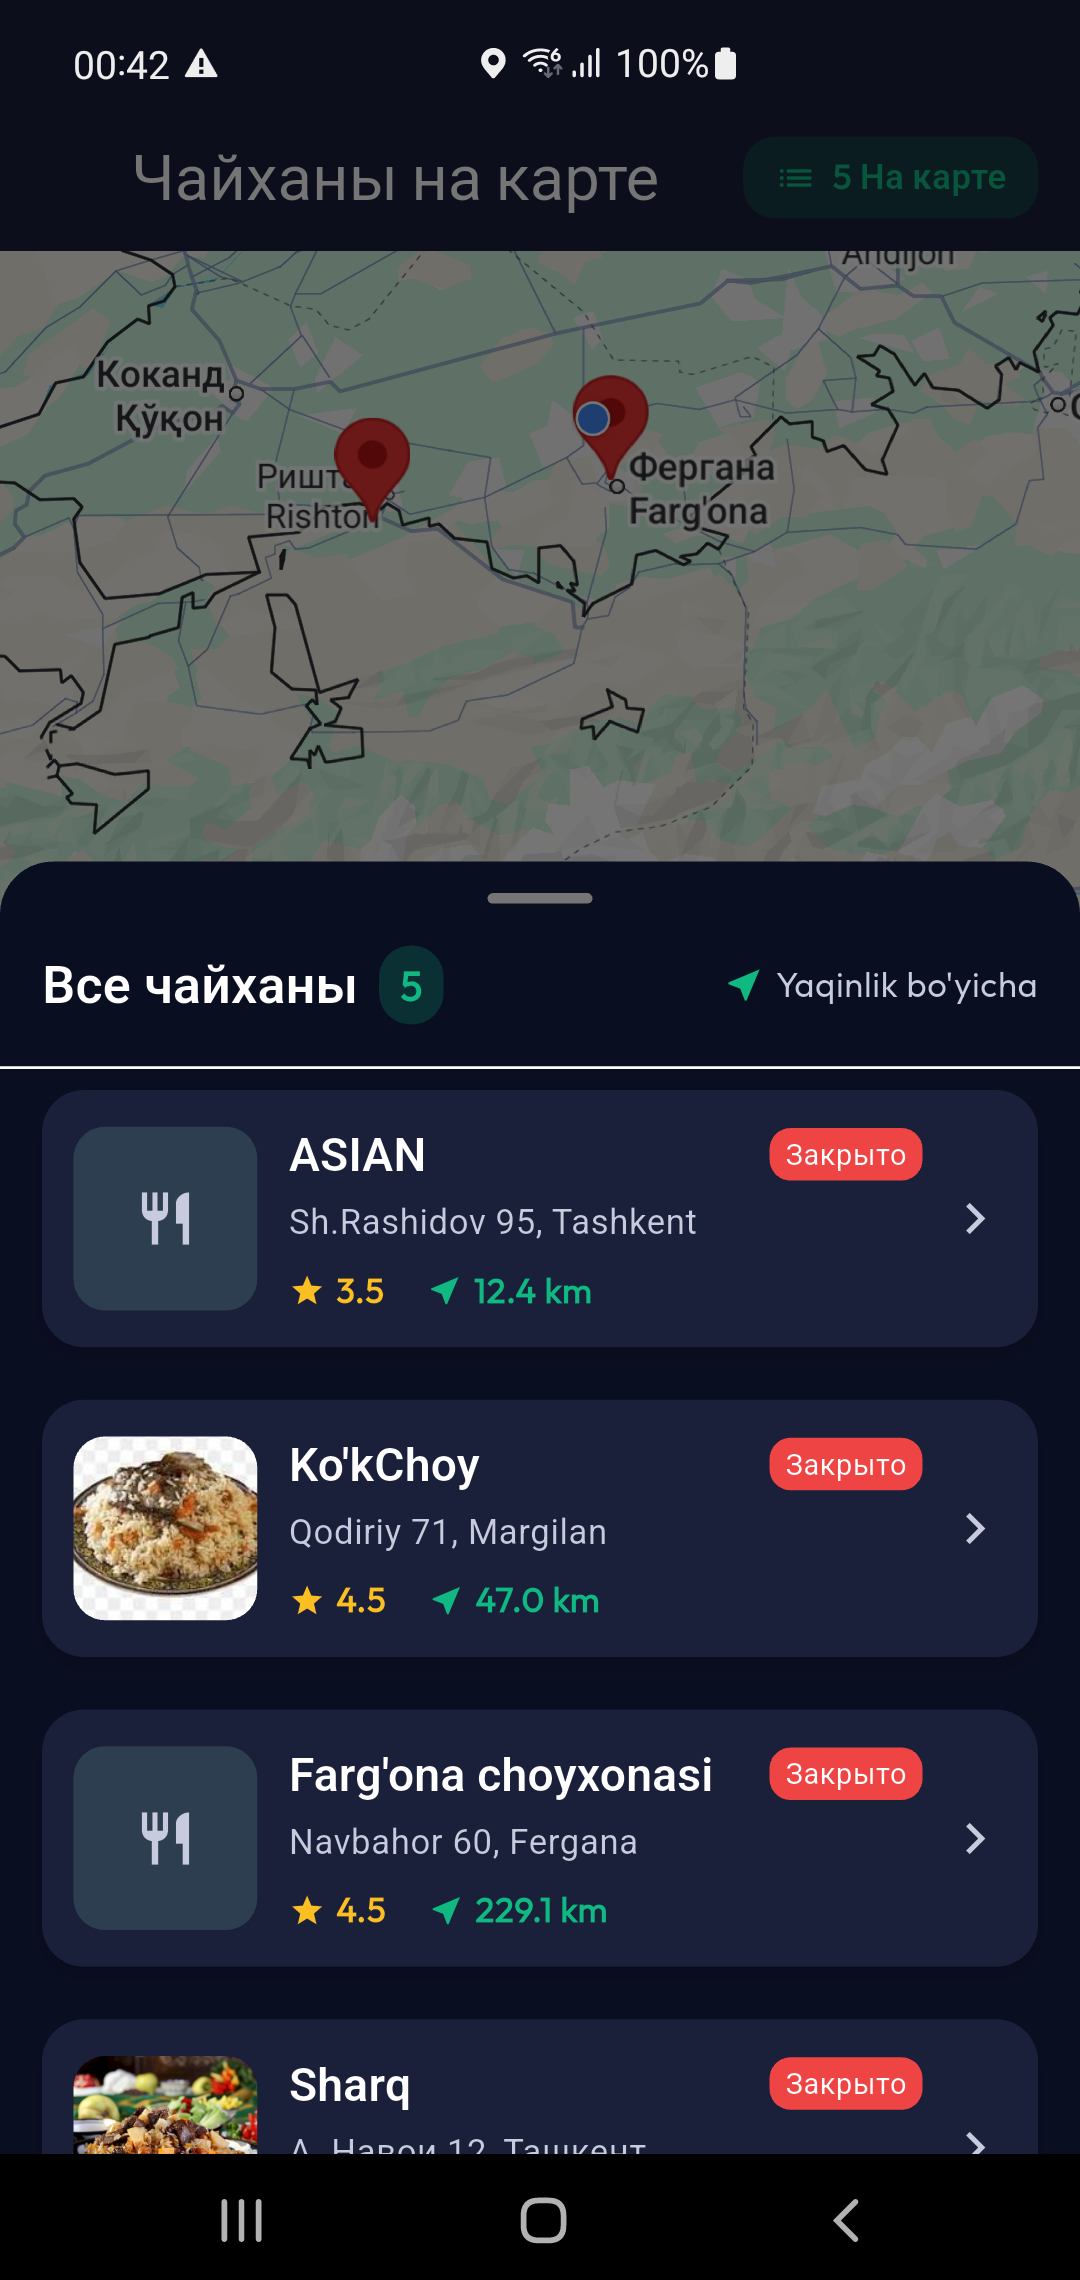
\includegraphics[width=0.4\textwidth]{b_chapters/chapter2/assets/google_maps.png}
  \figsource{CHOYXONA.UZ application screenshot.}
  \caption{Map interface showing establishment locations with markers across Uzbekistan.}
  \label{fig:google-maps}
\end{figure}

As shown in \cref{fig:google-maps}, establishment locations appear as markers positioned according to their geographic coordinates.
Custom marker images distinguish establishment types visually.
Tapping a marker displays an info window with essential information including name, rating, and price range, with navigation to the full detail screen.

Location services utilize the \texttt{geolocator} package to access the device's GPS.
Location access requires explicit user permission, handled through a permission request flow.
When granted, the user's current location becomes the default center for map views and basis for sorting by proximity.
Distance calculation employs the \textbf{Haversine formula} for great-circle distance between coordinates:

\begin{equation}
  d = 2r \cdot \arcsin\!\left(\sqrt{\sin^2\!\left(\frac{\varphi_2-\varphi_1}{2}\right) + \cos\varphi_1 \cdot \cos\varphi_2 \cdot \sin^2\!\left(\frac{\lambda_2-\lambda_1}{2}\right)}\right)
  \label{eq:haversine}
\end{equation}

\noindent where $r$ is Earth's radius, $\varphi$ is latitude, and $\lambda$ is longitude in radians.
This provides accurate measurements for the typical distances involved in local restaurant search.

\textbf{Region-based filtering} provides geographic organization without requiring location permission.
The application presents a region selector with major Uzbek cities: Tashkent, Samarkand, Bukhara, Namangan, Andijan, Fergana, and others.
This supports users planning visits to unfamiliar areas~\cite{jia2014}.

\textbf{Directions integration} constructs intent URIs that open external navigation applications (Google Maps on Android, Apple Maps on iOS), respecting user choice of navigation tools and providing full navigation functionality without duplicating turn-by-turn capabilities.

\begin{figure}[htbp]
  \centering
  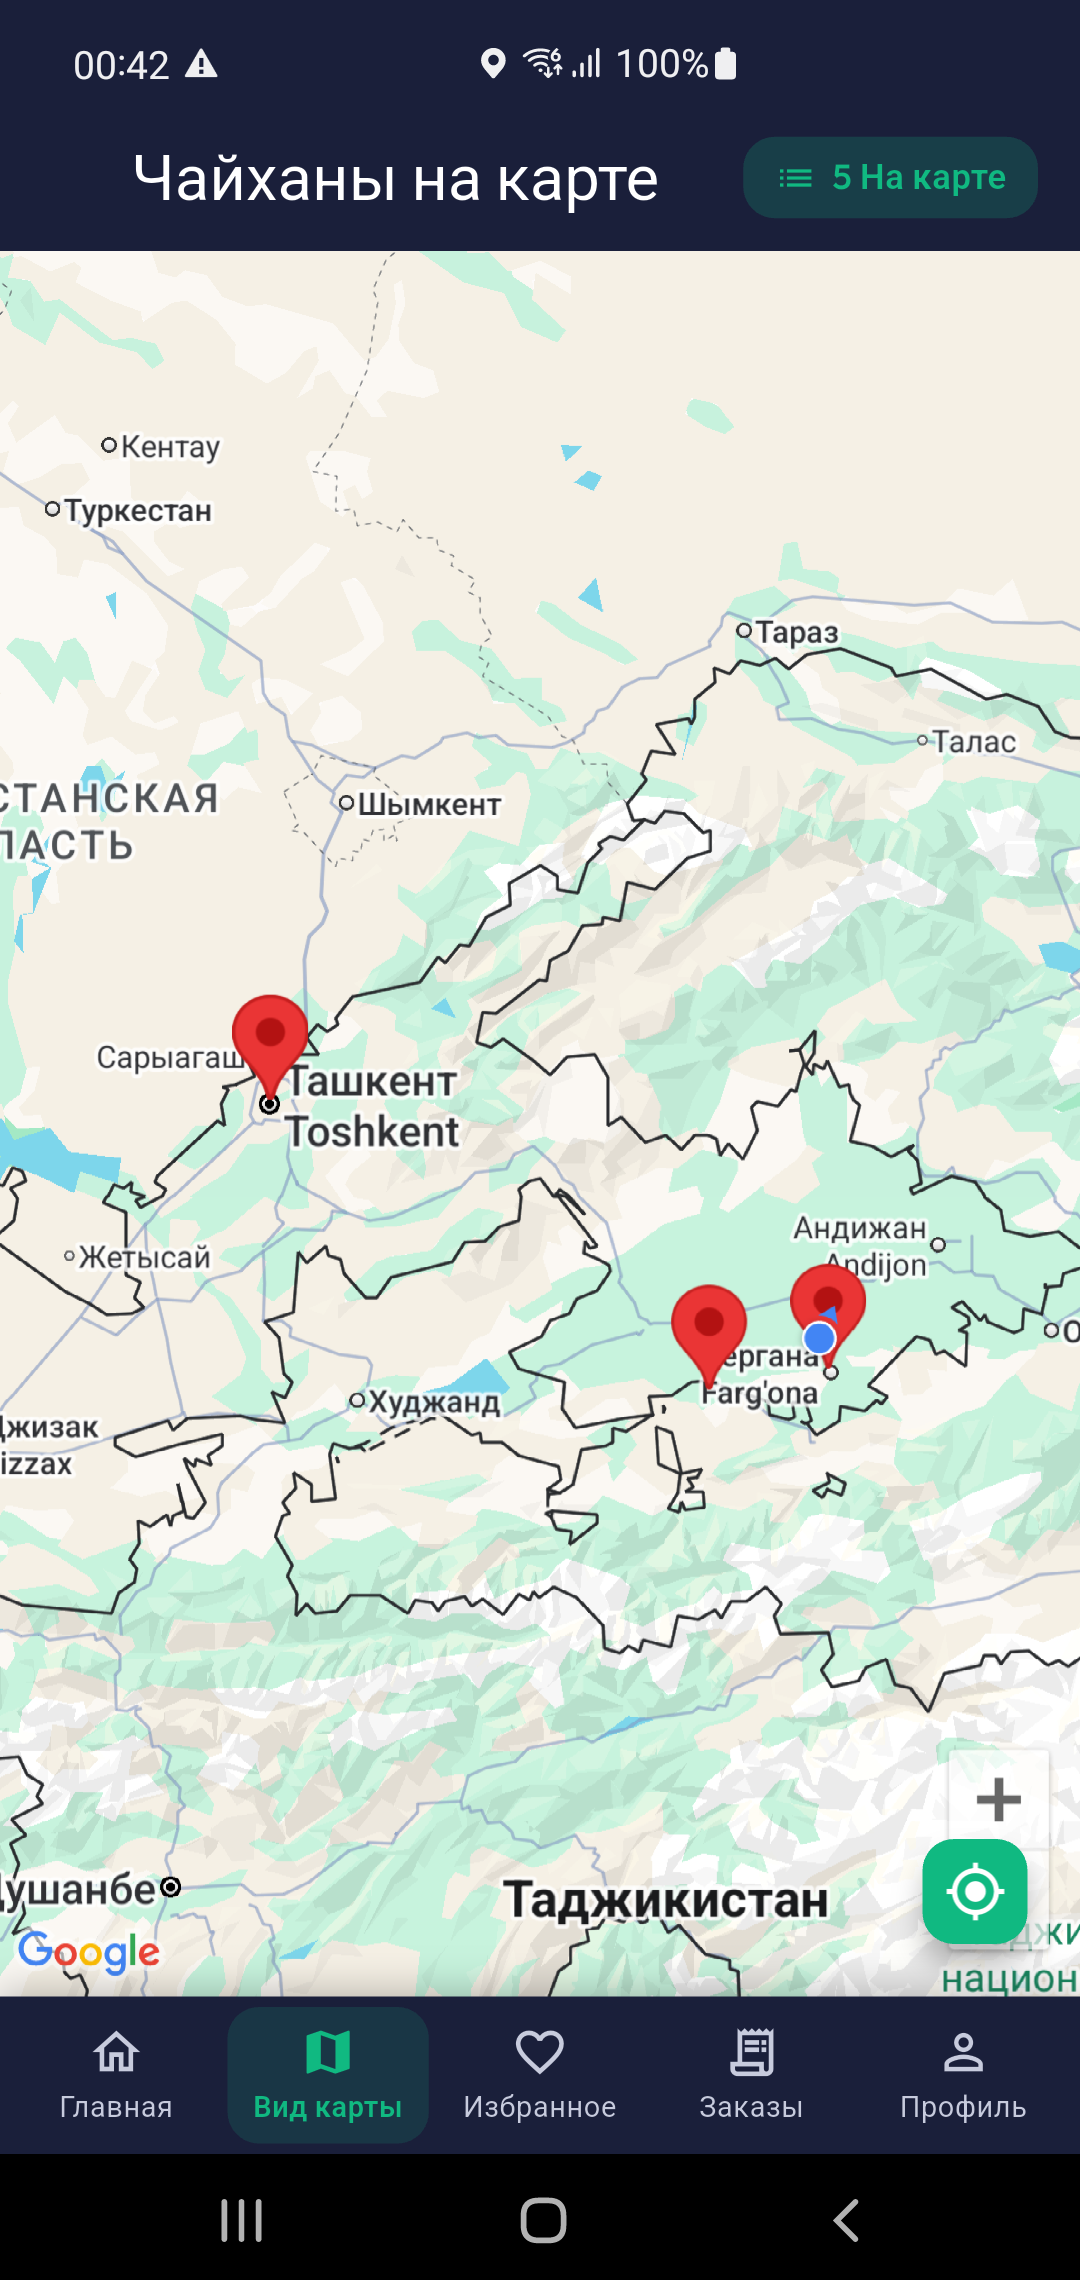
\includegraphics[width=0.4\textwidth]{b_chapters/chapter2/assets/screenshot_system.png}
  \figsource{CHOYXONA.UZ application screenshot.}
  \caption{Full-screen map view with bottom navigation bar showing the Map View tab active.}
  \label{fig:map-fullscreen}
\end{figure}

\cref{fig:map-fullscreen} demonstrates the full-screen map view with the bottom navigation bar.
Users can switch between list and map views while maintaining their current filters.
The map automatically positions to show all matching establishments, adjusting zoom level to fit results.


% =====================================================================
\section{Chapter Summary}
\label{sec:ch2-summary}

This chapter presented the technical foundation of the CHOYXONA.UZ application through five key areas:

First, \cref{sec:system-arch} described the three-layer architecture (presentation, business logic, data) that separates concerns and leverages Firebase's managed infrastructure to eliminate custom server maintenance.
The feature-based code organization ensures maintainability as the codebase grows.

Second, \cref{sec:database} detailed the Firestore data model with its primary collections (\texttt{users}, \texttt{choyxonas}, \texttt{bookings}, \texttt{reviews}), strategic denormalization for read optimization, composite indexing for multi-field queries, and role-based security rules enforcing authorization at the database level (\cref{tab:security-rules}).

Third, \cref{sec:ui-design} covered the Material Design~3 visual system with dual-theme support, bottom navigation architecture for five primary destinations, responsive layout breakpoints from compact phones to expanded tablets (\cref{tab:breakpoints}), and trilingual localization supporting Uzbek, Russian, and English.

Fourth, \cref{sec:realtime} explained the real-time synchronization mechanism using Firestore listeners and Flutter's \texttt{StreamBuilder}, the centralized \texttt{DataSyncProvider} for efficient stream sharing, offline persistence for unreliable connectivity, and transactional booking creation with optimistic updates.

Fifth, \cref{sec:maps} described Google Maps integration for geographic discovery, the Haversine formula for distance calculation (\cref{eq:haversine}), region-based filtering for planning scenarios, and external navigation app integration for directions.

These architectural foundations support the functional capabilities described in Chapter~3.

\chapter{Implementation and Functional Capabilities}
\label{ch:implementation}

This chapter details the functional capabilities of the CHOYXONA.UZ application across three user roles: customers, establishment administrators, and platform super administrators.
It covers the authentication and profile management module, the search-to-booking user journey, the administrator management dashboard, the super administrator platform oversight panel, and the notification system.
Each section includes screenshots from the implemented application demonstrating the described functionality.


% =====================================================================
\section{User Module: Registration and Authentication}
\label{sec:user-module}

The user module handles identity management throughout the application lifecycle, from initial registration through ongoing profile maintenance.
This foundational module ensures secure access to features while maintaining a frictionless onboarding experience~\cite{firebase_auth2024}.

\subsection{Authentication Methods}
\label{subsec:auth-methods}

CHOYXONA.UZ supports two primary authentication methods aligned with Uzbek user preferences:

\textbf{Email and password registration} provides the traditional account creation flow.
Users enter their email address, create a password meeting minimum complexity requirements (at least eight characters with mixed case and numbers), and confirm the password.
Upon successful registration, a verification email is sent, though the application permits limited functionality before verification to reduce onboarding friction~\cite{firebase_auth2024}.

\textbf{Phone number authentication} employs SMS-based one-time passwords (OTP).
Users enter their phone number in international format and receive a six-digit verification code via SMS.
This method is particularly relevant for the Uzbek market where phone numbers serve as primary identifiers~\cite{khawas2018}.

The application startup and authentication flow is illustrated in \cref{fig:splash-auth}.

\begin{figure}[htbp]
  \centering
  \begin{minipage}[b]{0.3\textwidth}
    \centering
    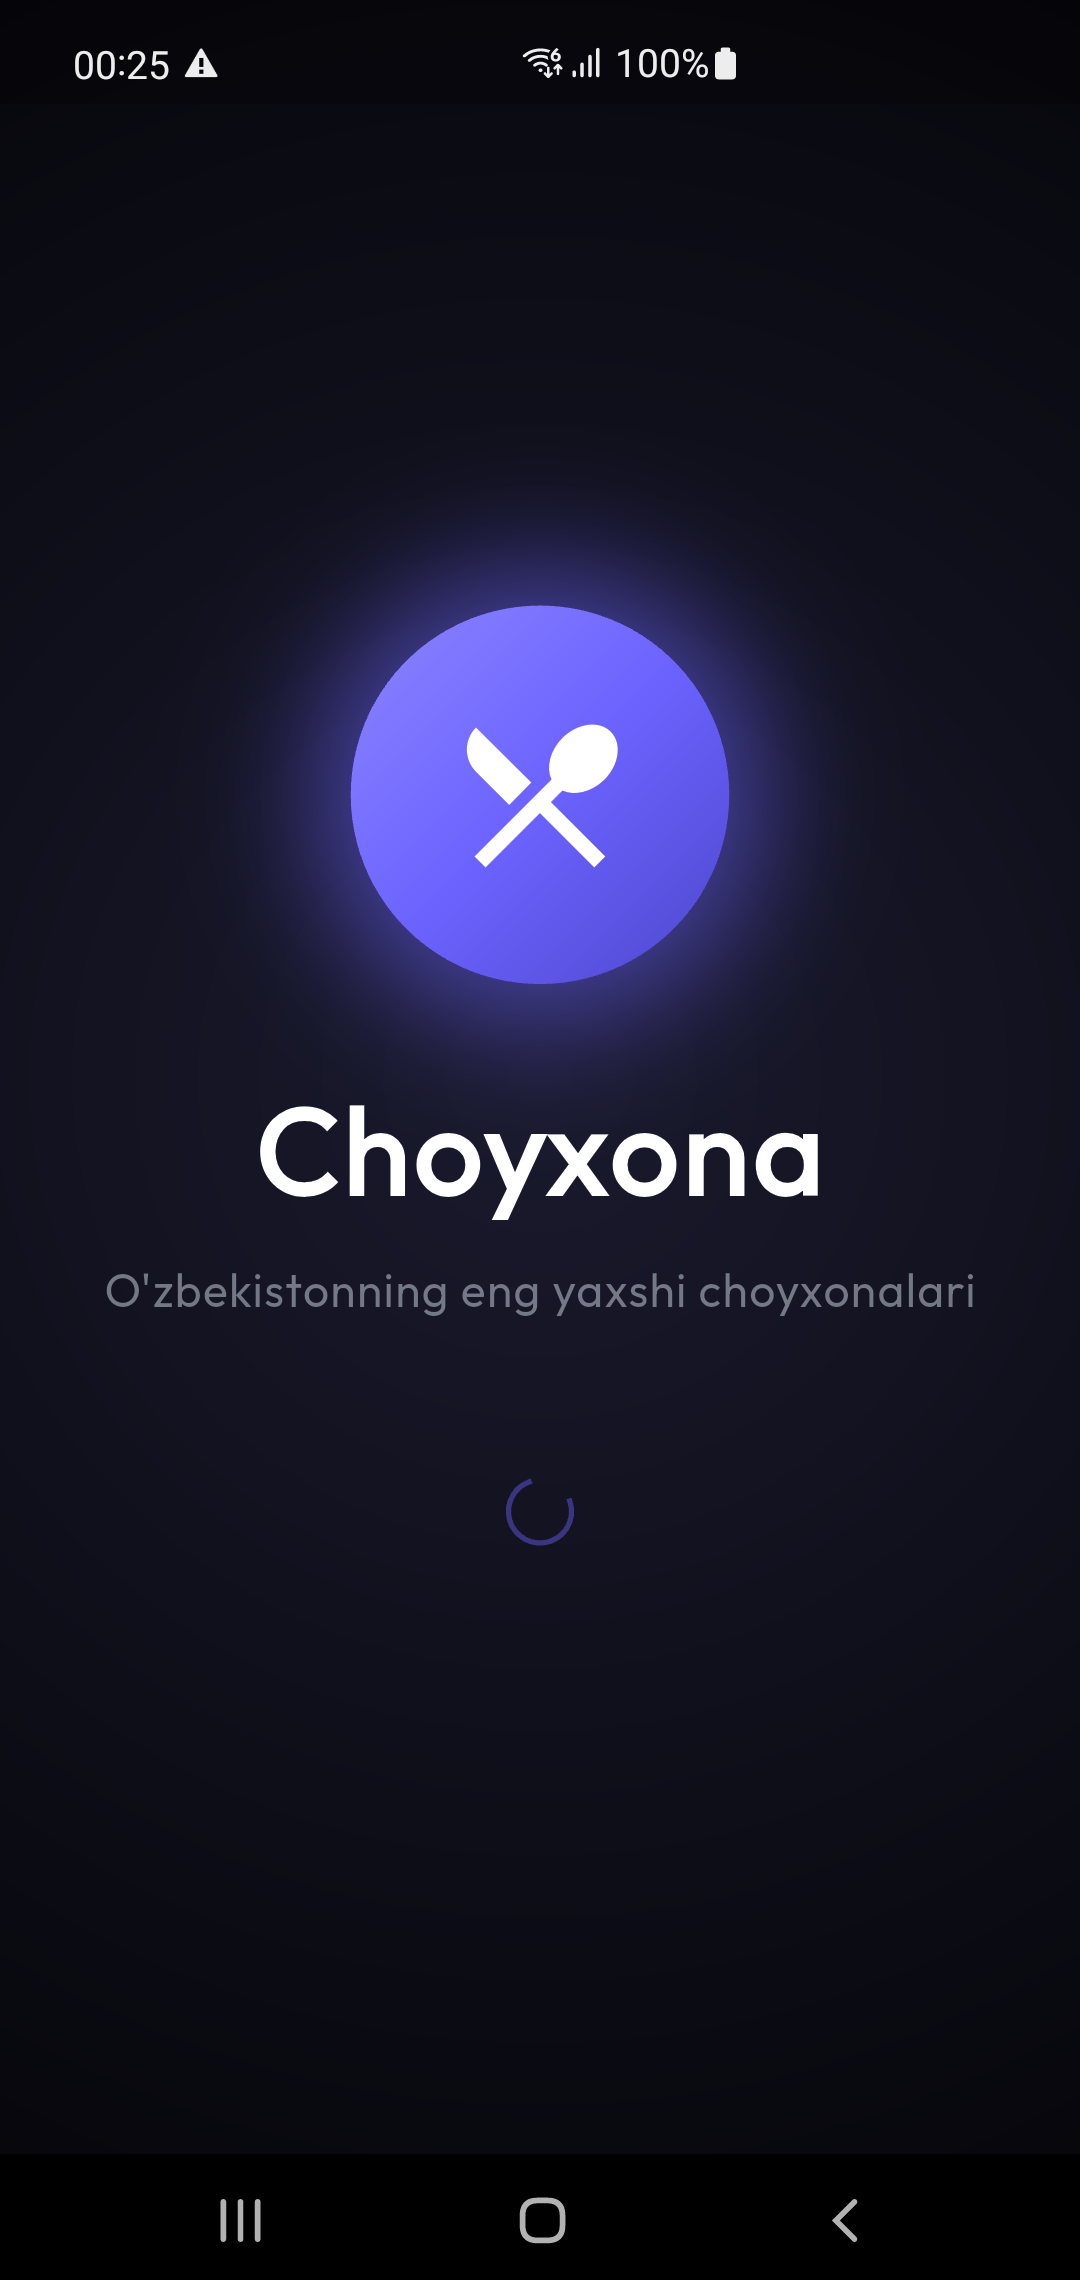
\includegraphics[width=\textwidth]{b_chapters/chapter3/assets/splash_screen.png}
  \end{minipage}
  \hfill
  \begin{minipage}[b]{0.3\textwidth}
    \centering
    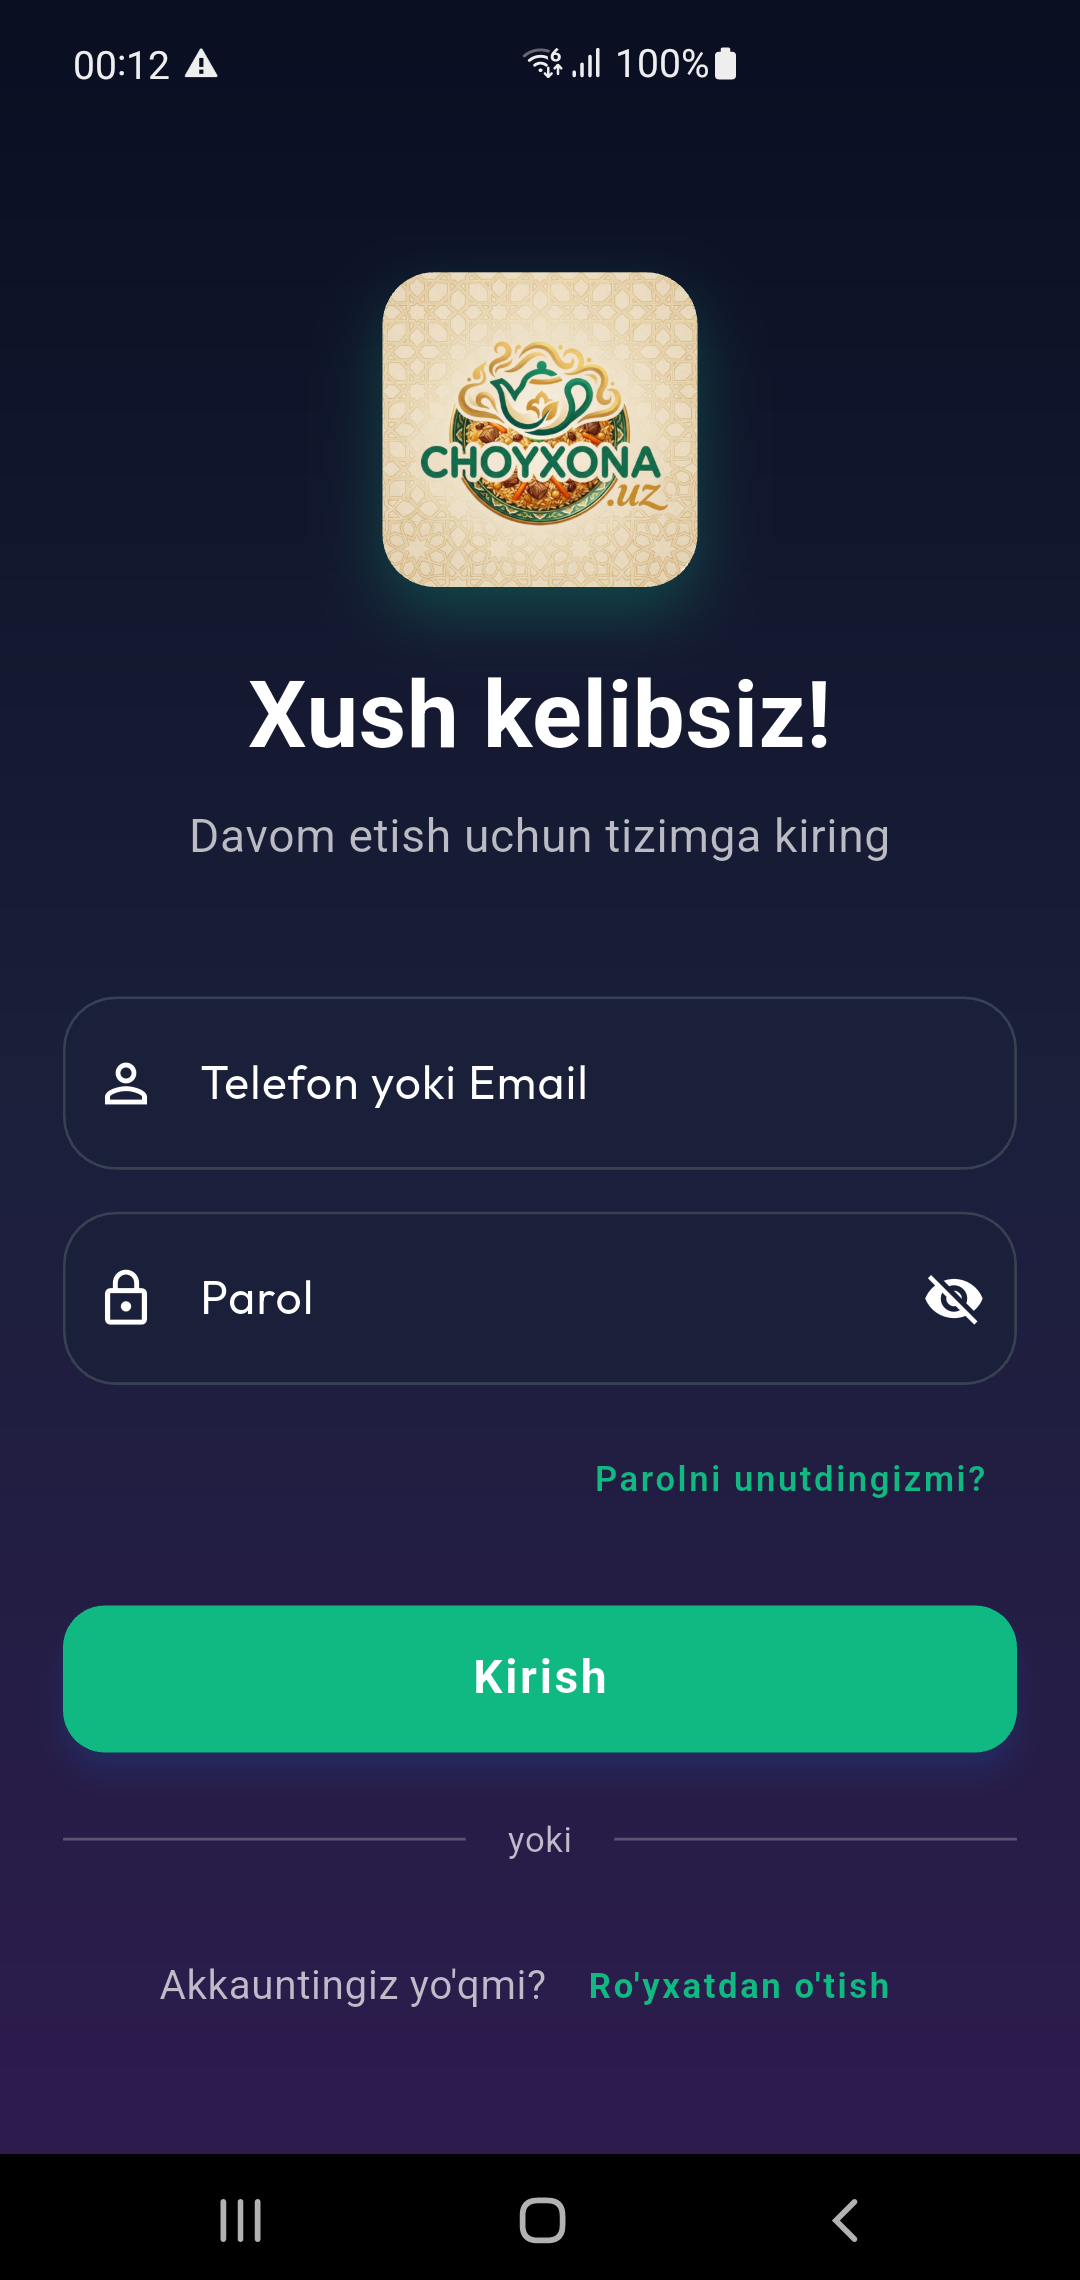
\includegraphics[width=\textwidth]{b_chapters/chapter3/assets/auth_screen.png}
  \end{minipage}
  \hfill
  \begin{minipage}[b]{0.3\textwidth}
    \centering
    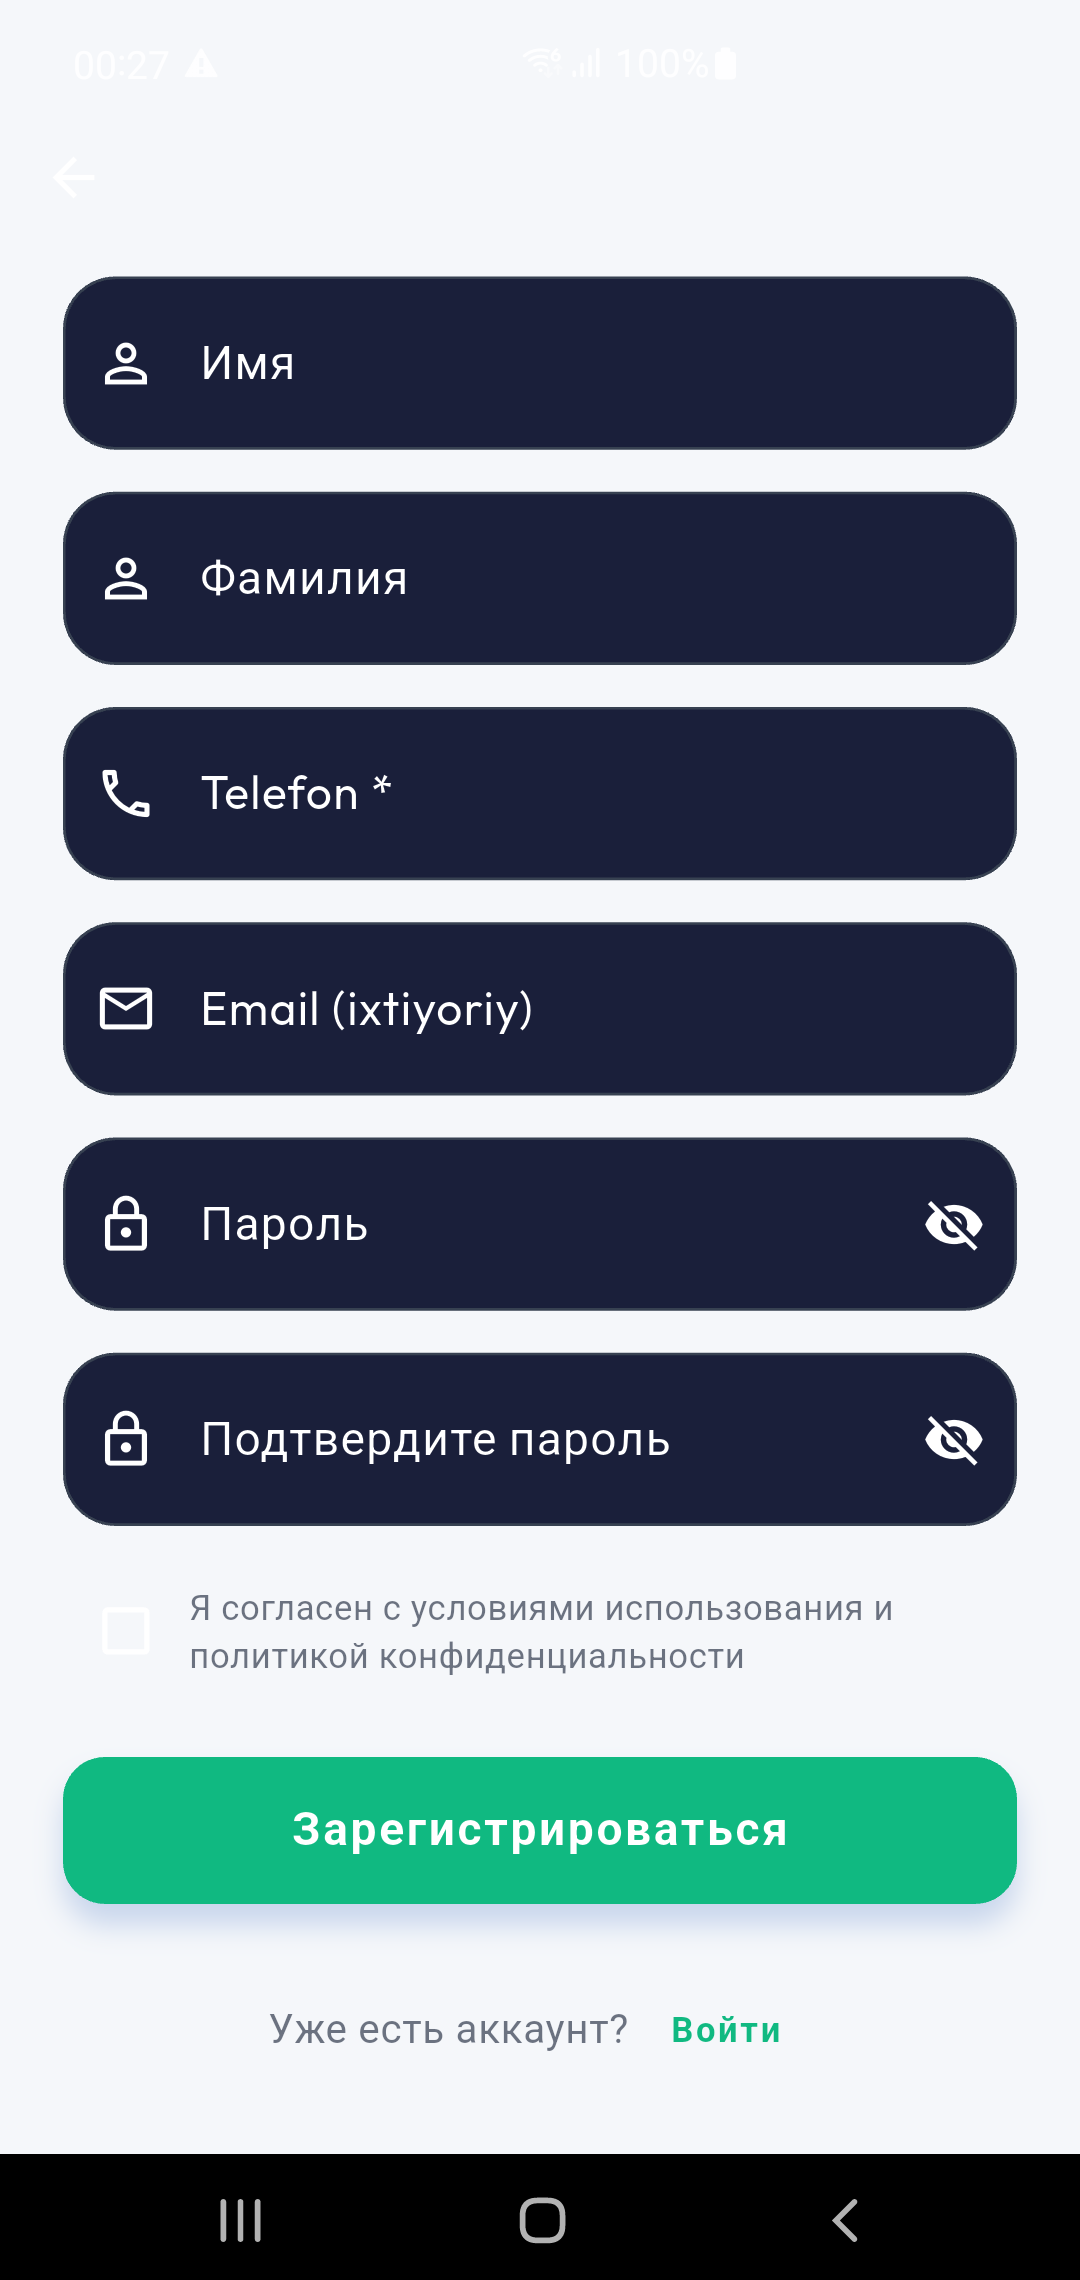
\includegraphics[width=\textwidth]{b_chapters/chapter3/assets/regist_screen.png}
  \end{minipage}
  \figsource{CHOYXONA.UZ application screenshots.}
  \caption{Application flow: splash screen (left), login screen (center), and registration screen (right).}
  \label{fig:splash-auth}
\end{figure}

The \texttt{auth\_service.dart} file encapsulates all Firebase Authentication interactions behind a clean interface, exposing methods including:
\begin{itemize}
  \item \texttt{signInWithEmail()} --- authenticates using email and password credentials;
  \item \texttt{signInWithPhone()} --- initiates and completes phone verification;
  \item \texttt{signOut()} --- ends the session and clears cached data;
  \item \texttt{resetPassword()} --- sends password reset instructions;
  \item \texttt{updatePassword()} --- changes the password for the current user.
\end{itemize}

The \texttt{authStateChanges} stream provides reactive authentication state.
The splash screen subscribes to this stream to determine whether to navigate to the login screen or the main application.
The \texttt{RoleBasedNavigator} component uses authentication state combined with role information to direct users to the appropriate interface~\cite{flutter_state2024}.

\subsection{Role-Based Access Control}
\label{subsec:rbac}

Three primary roles determine feature availability:
\begin{enumerate}
  \item \textbf{User} (customer) --- discovers establishments, makes bookings, and leaves reviews.
  \item \textbf{Admin} (establishment administrator) --- manages a specific establishment; their user document includes an establishment reference.
  \item \textbf{Super Admin} --- oversees the entire platform with access to user management, establishment verification, and system configuration.
\end{enumerate}

Role assignment occurs automatically during registration (as ``user''). Administrator roles are assigned by super administrators through the user management interface.
The role-based routing flow is illustrated in \cref{fig:role-routing}.

\begin{figure}[htbp]
  \centering
  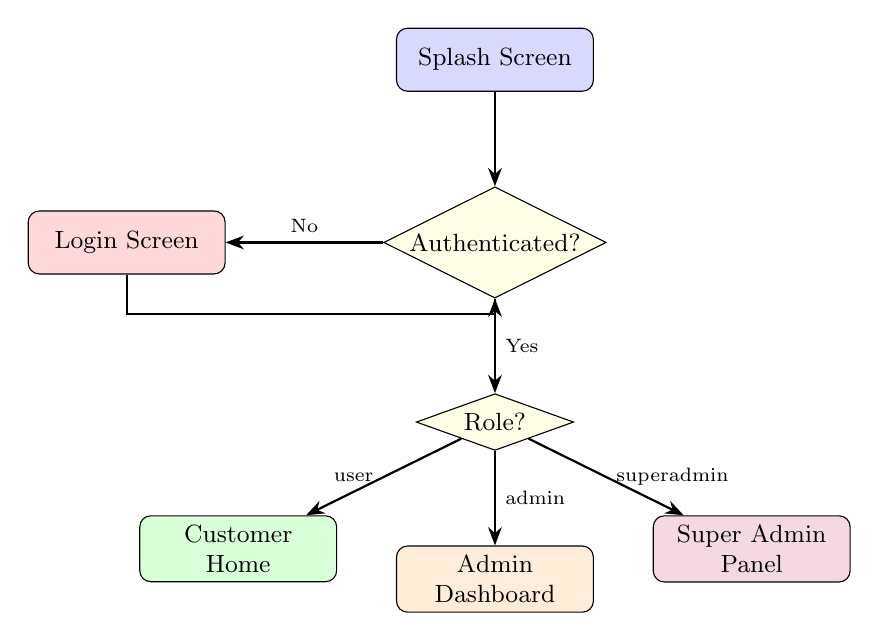
\begin{tikzpicture}[
    box/.style={draw, rounded corners=4pt, minimum width=2.5cm, minimum height=0.8cm, align=center, font=\small, fill=#1!15},
    decision/.style={draw, diamond, aspect=2, minimum width=2cm, inner sep=1pt, font=\small, fill=yellow!10},
    arr/.style={->, thick, >=Stealth},
    node distance=1.2cm
  ]
    \node[box=blue] (splash) {Splash Screen};
    \node[decision, below=of splash] (auth) {Authenticated?};
    \node[box=red, left=2cm of auth] (login) {Login Screen};
    \node[decision, below=of auth] (role) {Role?};
    \node[box=green, below left=1cm and 1.5cm of role] (user) {Customer\\Home};
    \node[box=orange, below=of role] (admin) {Admin\\Dashboard};
    \node[box=purple, below right=1cm and 1.5cm of role] (super) {Super Admin\\Panel};

    \draw[arr] (splash) -- (auth);
    \draw[arr] (auth) -- node[above,font=\scriptsize]{No} (login);
    \draw[arr] (auth) -- node[right,font=\scriptsize]{Yes} (role);
    \draw[arr] (role) -- node[left,font=\scriptsize]{user} (user);
    \draw[arr] (role) -- node[right,font=\scriptsize]{admin} (admin);
    \draw[arr] (role) -- node[right,font=\scriptsize]{superadmin} (super);
    \draw[arr] (login.south) |- ++(0,-0.5) -| (auth);
  \end{tikzpicture}
  \caption{Role-based navigation routing from splash screen to role-specific interfaces.}
  \label{fig:role-routing}
\end{figure}

\subsection{Profile Management and Security}
\label{subsec:profile-security}

The profile management screen enables users to view and update personal information: profile photo (with camera capture or gallery selection, compressed before upload to Cloud Storage), display name, phone number (requiring re-verification), language preference, and notification settings.
Preferences synchronize across devices through Firestore~\cite{firebase_firestore2024}.

Security considerations include: passwords never stored locally (only session tokens managed by Firebase SDK), sensitive operations requiring recent authentication, rate limiting on Firebase servers preventing brute-force attacks, and automatic account lockout after repeated failed attempts~\cite{firebase_auth2024}.


% =====================================================================
\section{Search, Filtering, and Booking Process}
\label{sec:search-booking}

The discovery and booking flow represents the core user journey, taking users from initial exploration through confirmed reservation.

\subsection{Discovery and Search}
\label{subsec:discovery}

The \textbf{home screen} combines curated content with personalized recommendations.
A search bar provides quick text access, a horizontal carousel displays featured establishments, and personalized recommendations appear based on user history~\cite{nielsen2012}.

The \textbf{search screen} offers comprehensive multi-dimensional filtering:

\begin{table}[htbp]
\caption{Search filter dimensions and available options}
\label{tab:search-filters}
\centering
\small
\begin{tabular}{lp{8cm}}
\toprule
\textbf{Filter} & \textbf{Options} \\
\midrule
Text search     & Name, description, and tag matching \\
Category        & Traditional teahouse, National cuisine, European, Mixed menu \\
Price range     & Budget-friendly ($), Moderate (\$\$), Upscale (\$\$\$) \\
Rating          & Minimum 3 stars, Minimum 4 stars \\
Location        & Region dropdown (Tashkent, Samarkand, Bukhara, etc.) \\
Distance        & Radius from current location (requires GPS permission) \\
Sorting         & Relevance, Distance, Rating, Newest \\
\bottomrule
\end{tabular}
\end{table}

Results display as scrollable \texttt{ChoyxonaCard} widgets with establishment image, name, star rating with review count, price indicator, and distance.
The list supports infinite scroll with lazy loading.
The customer-facing interface is shown in \cref{fig:user-interface}.

\begin{figure}[htbp]
  \centering
  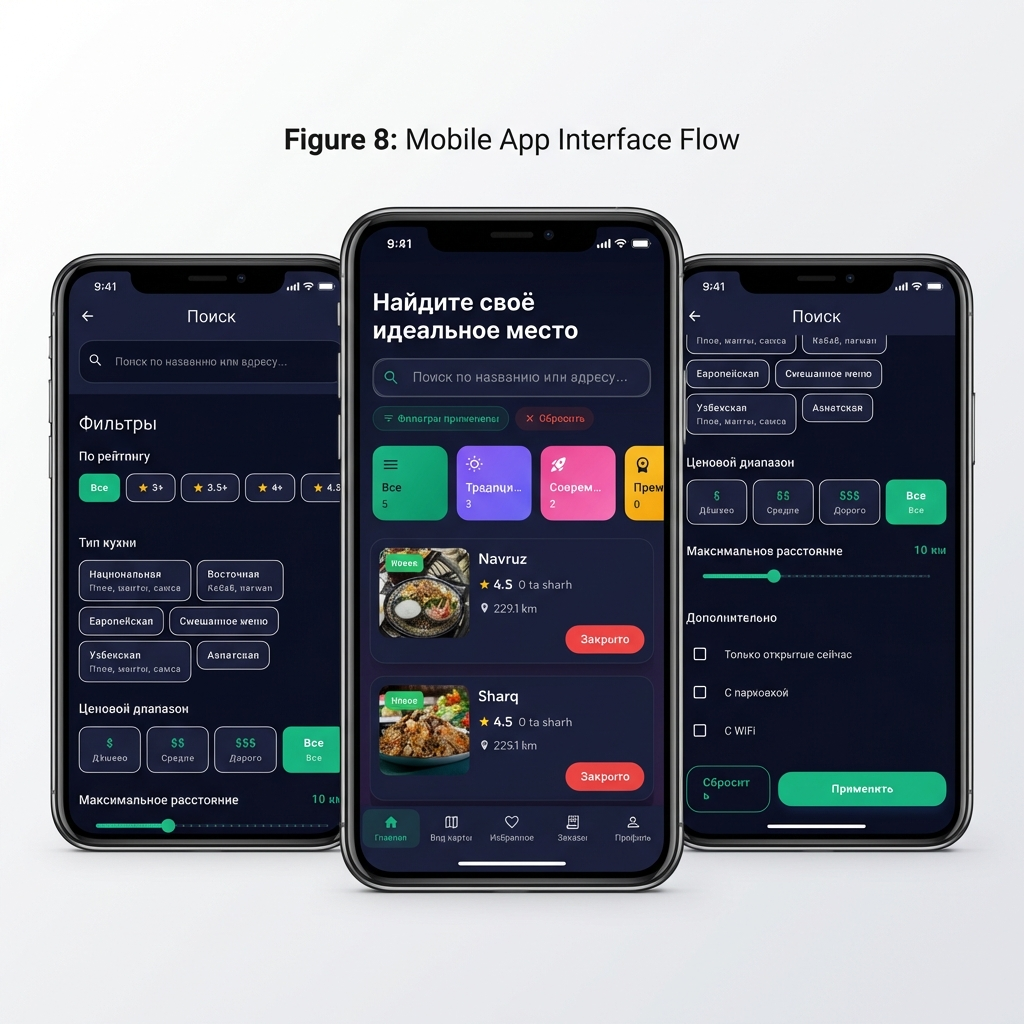
\includegraphics[width=0.7\textwidth]{b_chapters/chapter3/assets/user_collage.png}
  \figsource{CHOYXONA.UZ application screenshots.}
  \caption{Customer interface overview: home screen with featured establishments, search results, and establishment detail view.}
  \label{fig:user-interface}
\end{figure}

The \textbf{establishment detail screen} organizes information into tabbed sections: Overview (description, amenities, features), Menu (food and beverage with photos, prices, and categories loaded from subcollection), and Reviews (user feedback with ratings and text, sorted by recency or helpfulness).

\subsection{Booking Process}
\label{subsec:booking-process}

The booking process guides users through a structured four-step flow, as shown in \cref{fig:booking-flow}.

\begin{figure}[htbp]
  \centering
  \begin{minipage}[b]{0.3\textwidth}
    \centering
    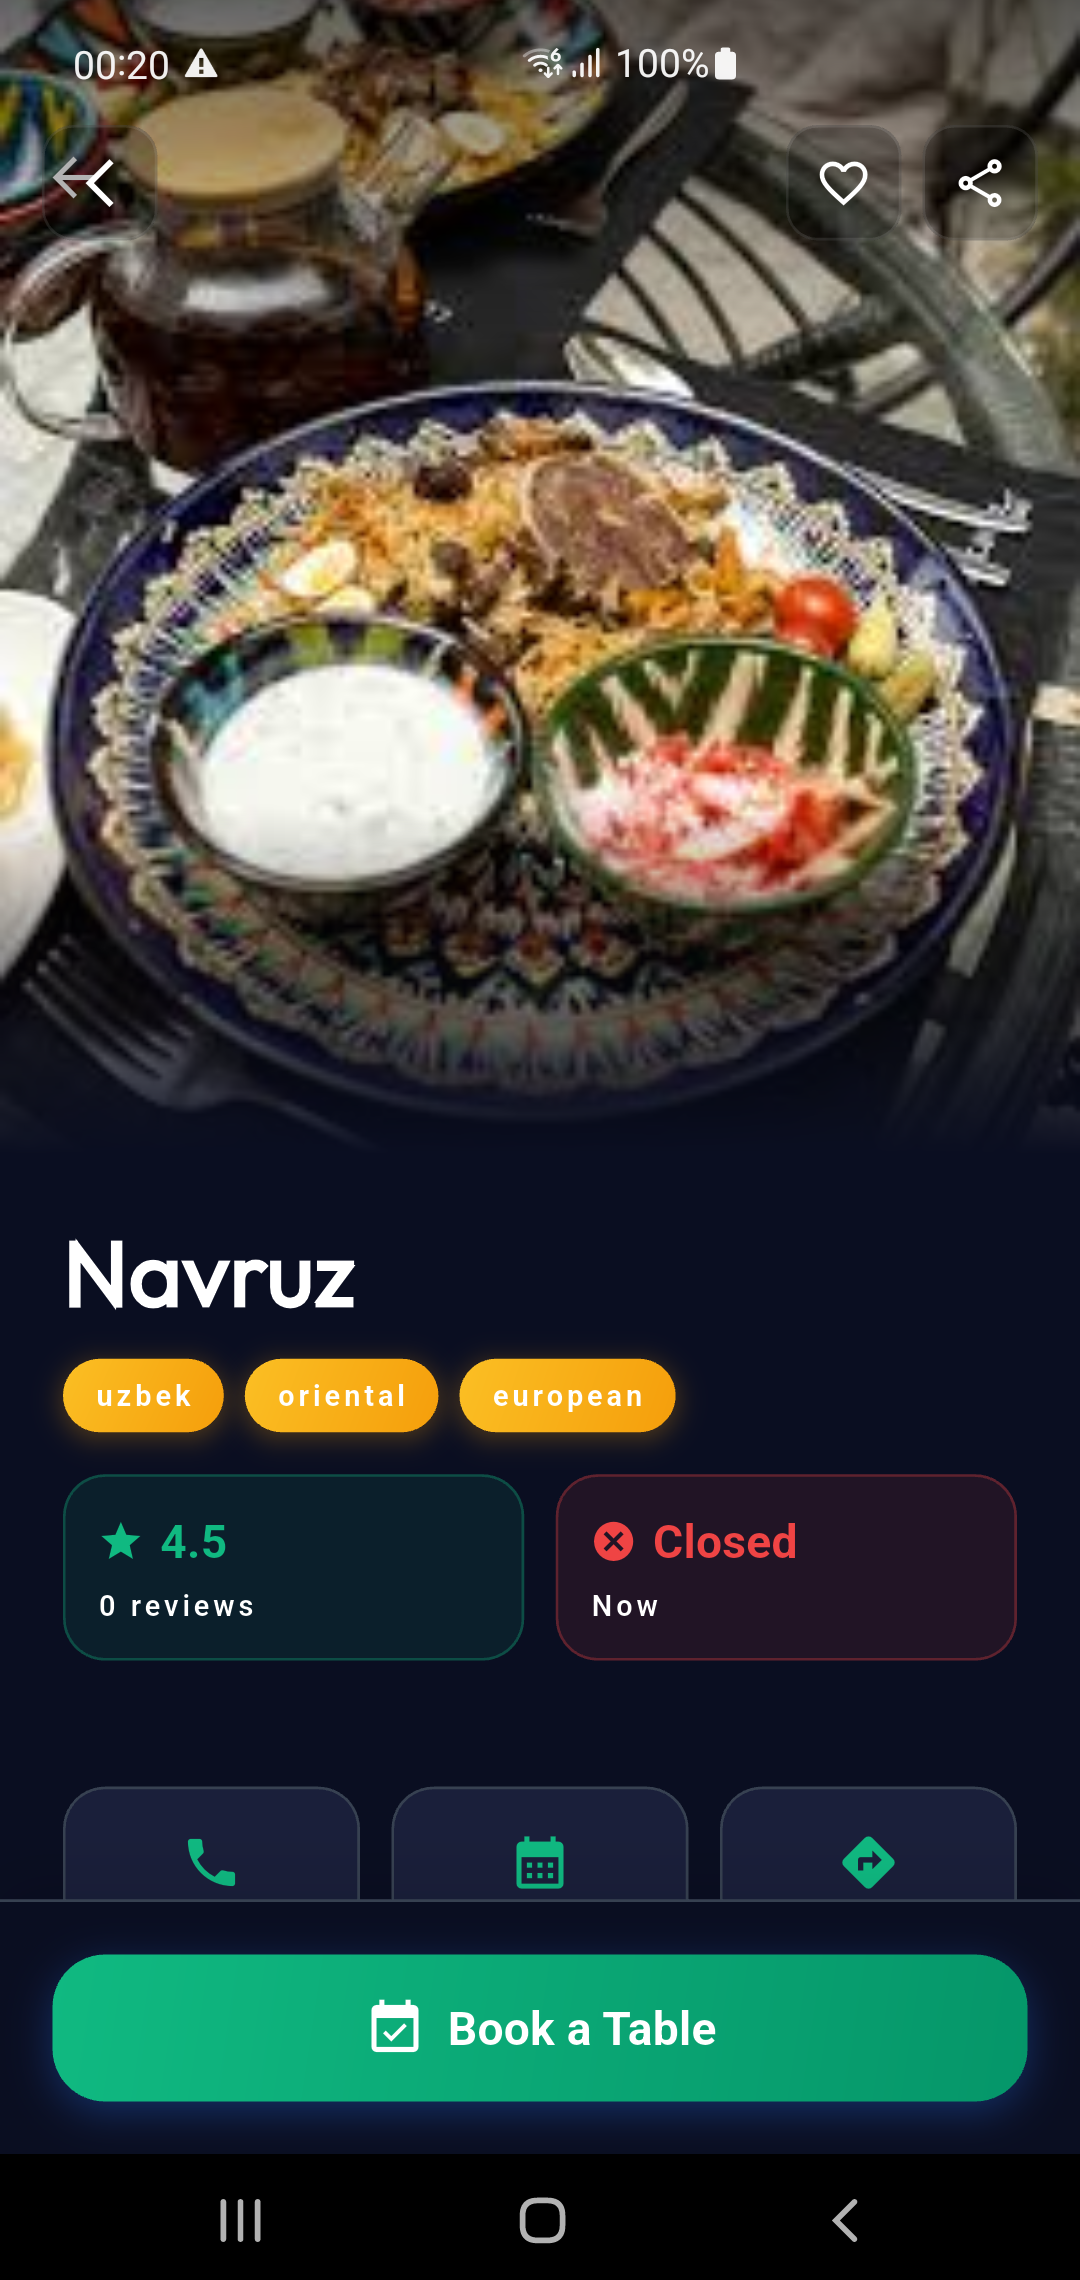
\includegraphics[width=\textwidth]{b_chapters/chapter3/assets/booking_step1.png}
  \end{minipage}
  \hfill
  \begin{minipage}[b]{0.3\textwidth}
    \centering
    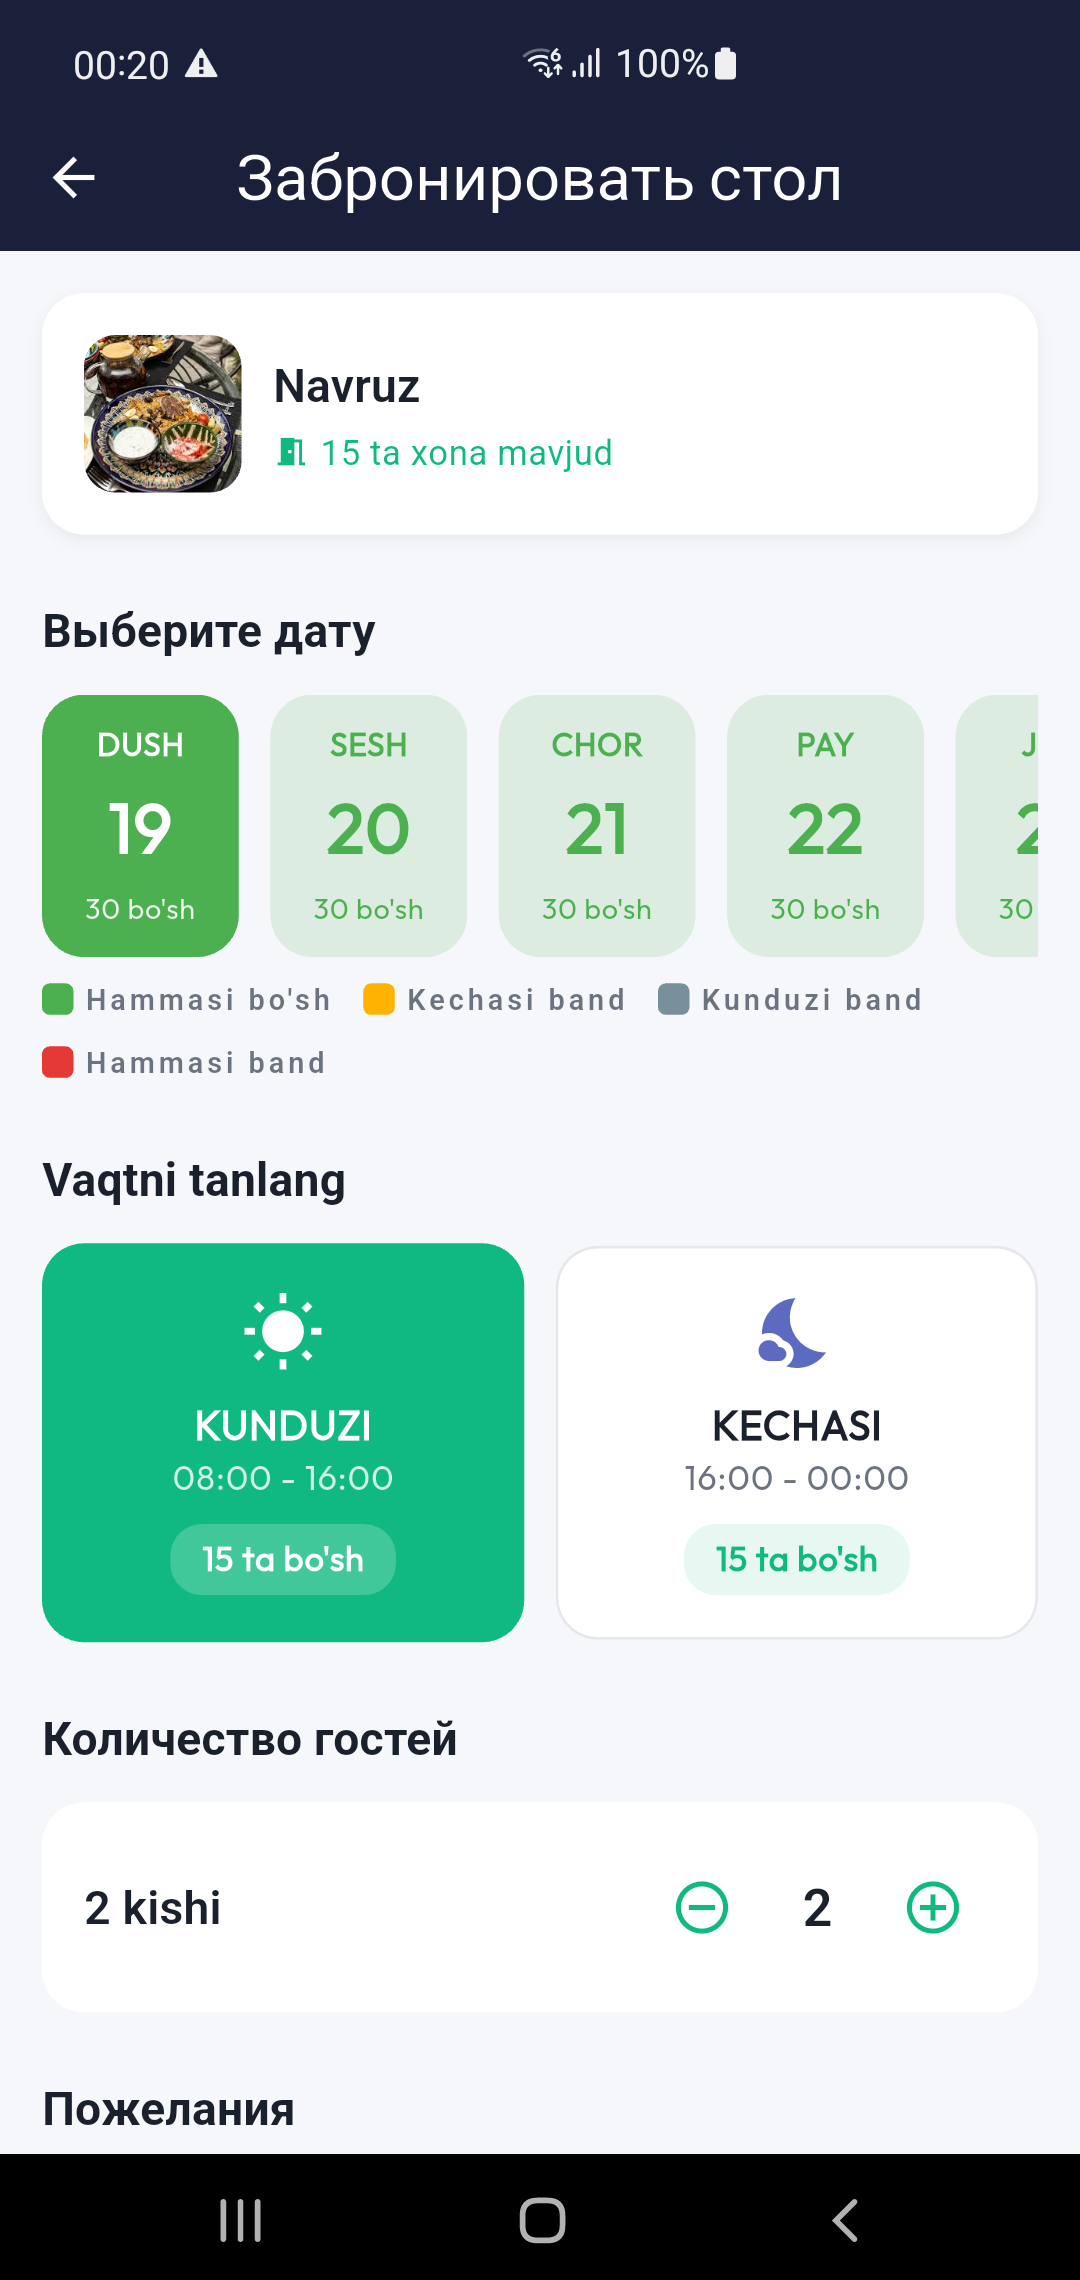
\includegraphics[width=\textwidth]{b_chapters/chapter3/assets/booking_step2.png}
  \end{minipage}
  \hfill
  \begin{minipage}[b]{0.3\textwidth}
    \centering
    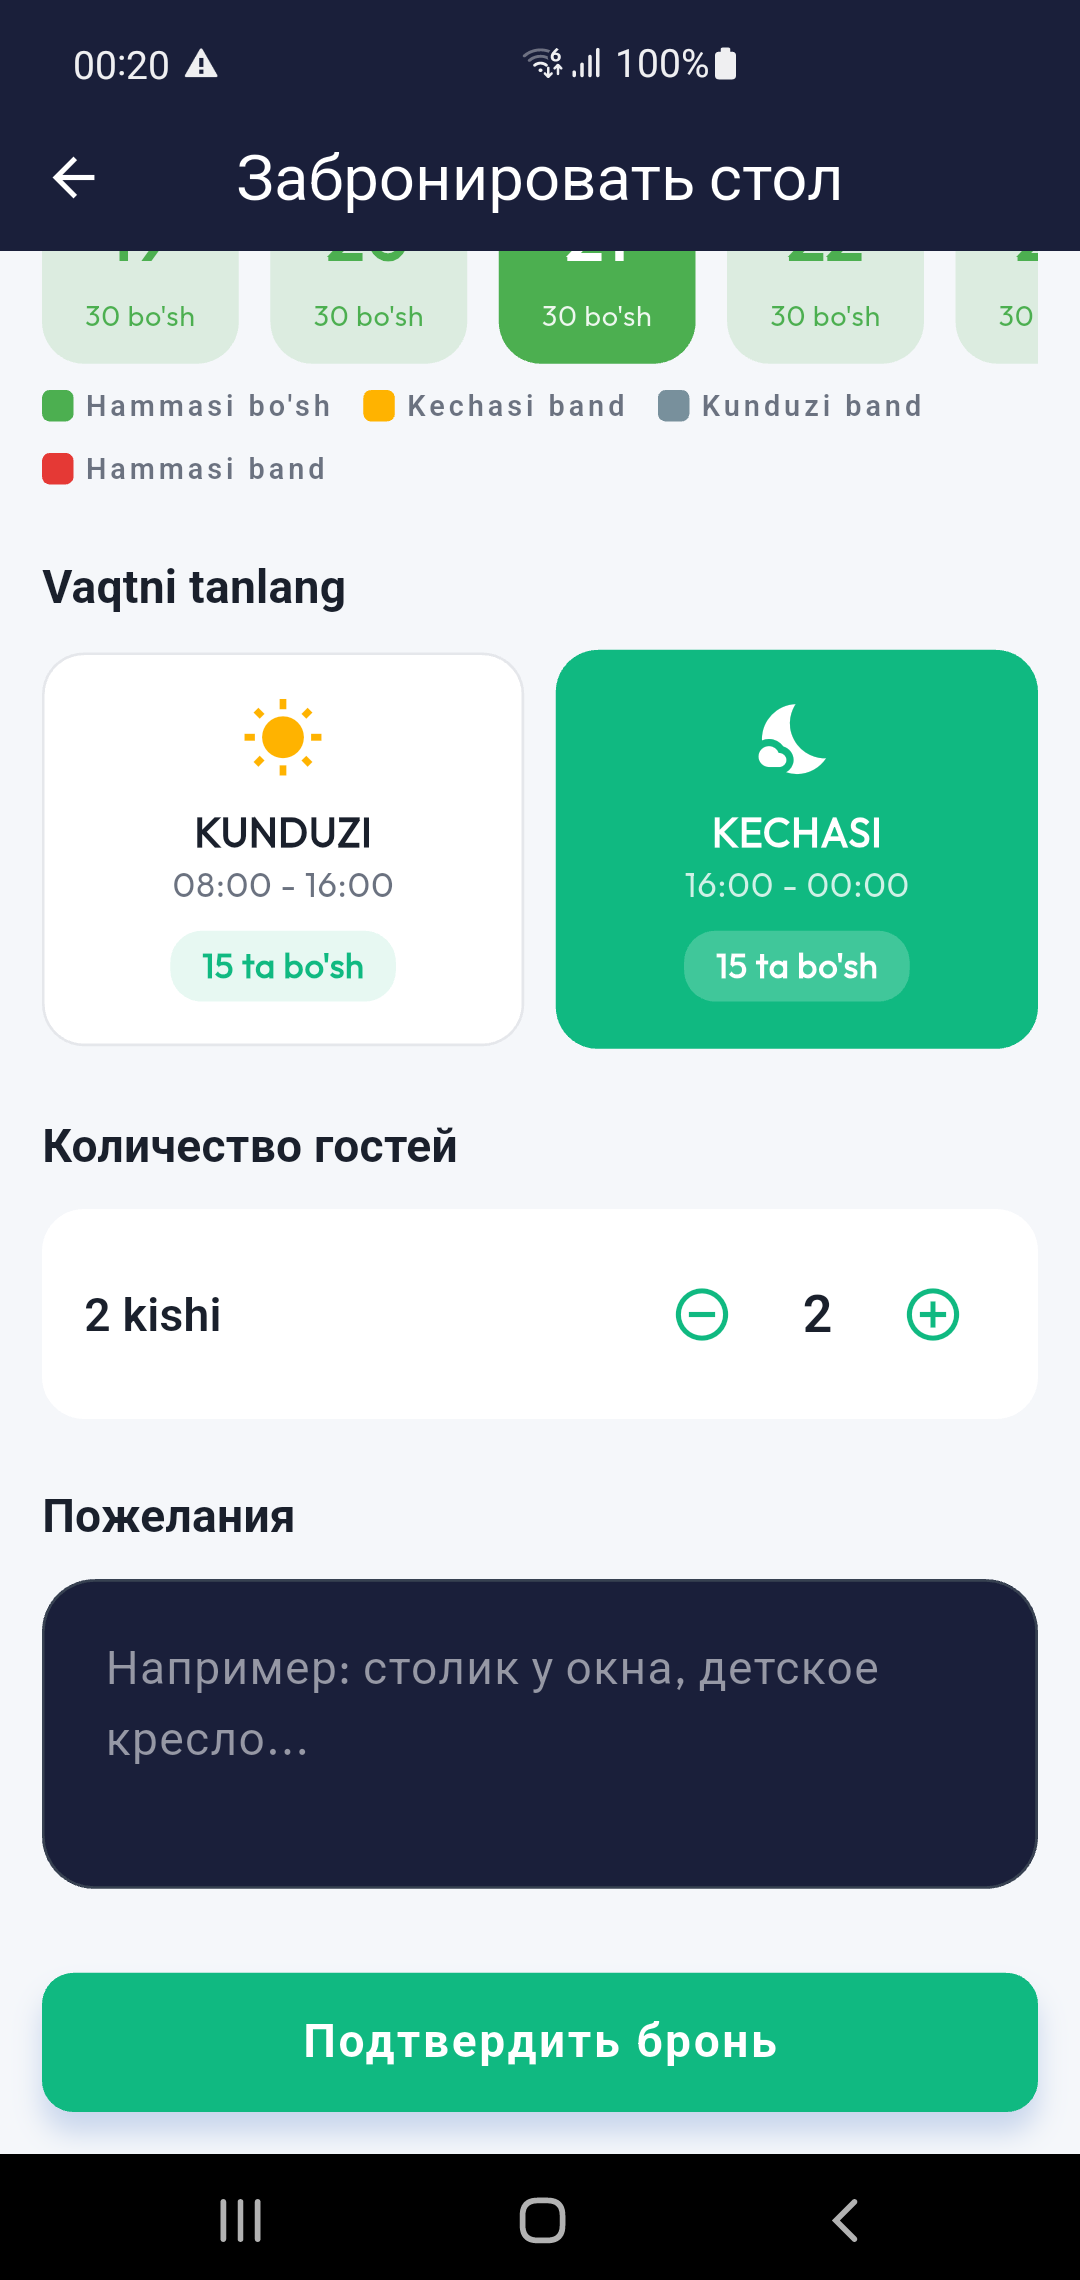
\includegraphics[width=\textwidth]{b_chapters/chapter3/assets/booking_step3.png}
  \end{minipage}
  \figsource{CHOYXONA.UZ application screenshots.}
  \caption{Booking process: date and time selection (left), party details and room preference (center), and booking confirmation (right).}
  \label{fig:booking-flow}
\end{figure}

The booking steps are:

\textbf{Step~1: Date selection.}
A calendar interface highlights dates with available slots while dimming fully booked dates.
Users cannot select past dates or dates beyond the establishment's advance booking window.

\textbf{Step~2: Time slot selection.}
Available slots for the chosen date display as tappable buttons with color-coded availability: green (fully available), yellow (limited availability), hidden (fully booked).
Slots are generated based on the establishment's configured duration and capacity.

\textbf{Step~3: Party details and room preference.}
A numeric stepper adjusts guest count within the establishment's limits.
For establishments offering private rooms (\textit{xona}), available room options show name, capacity, fee, and thumbnail.
Users can select a specific room or indicate no preference.

\textbf{Step~4: Confirmation.}
A summary of all selections appears for review.
Users can add special requests (dietary requirements, celebrations, seating preferences).
Cancellation policy terms require acknowledgment via checkbox~\cite{sommerville2015}.

Upon confirmation, the booking is submitted through a \textbf{Firestore transaction} that atomically verifies availability and creates the booking document.
If a conflict exists, the user is returned to time selection.
Successful bookings generate a unique reference code and QR code for quick check-in.
A push notification confirms the reservation immediately~\cite{firebase_firestore2024}.

\textbf{Booking management} enables users to view (upcoming/past sections), cancel (with reason prompt), or modify reservations.
A ``book again'' feature pre-fills details from previous visits for convenience.


% =====================================================================
\section{Administrator Panel}
\label{sec:admin-panel}

Establishment administrators access specialized management tools through a dedicated dashboard, as shown in \cref{fig:admin-dashboard}.

\begin{figure}[htbp]
  \centering
  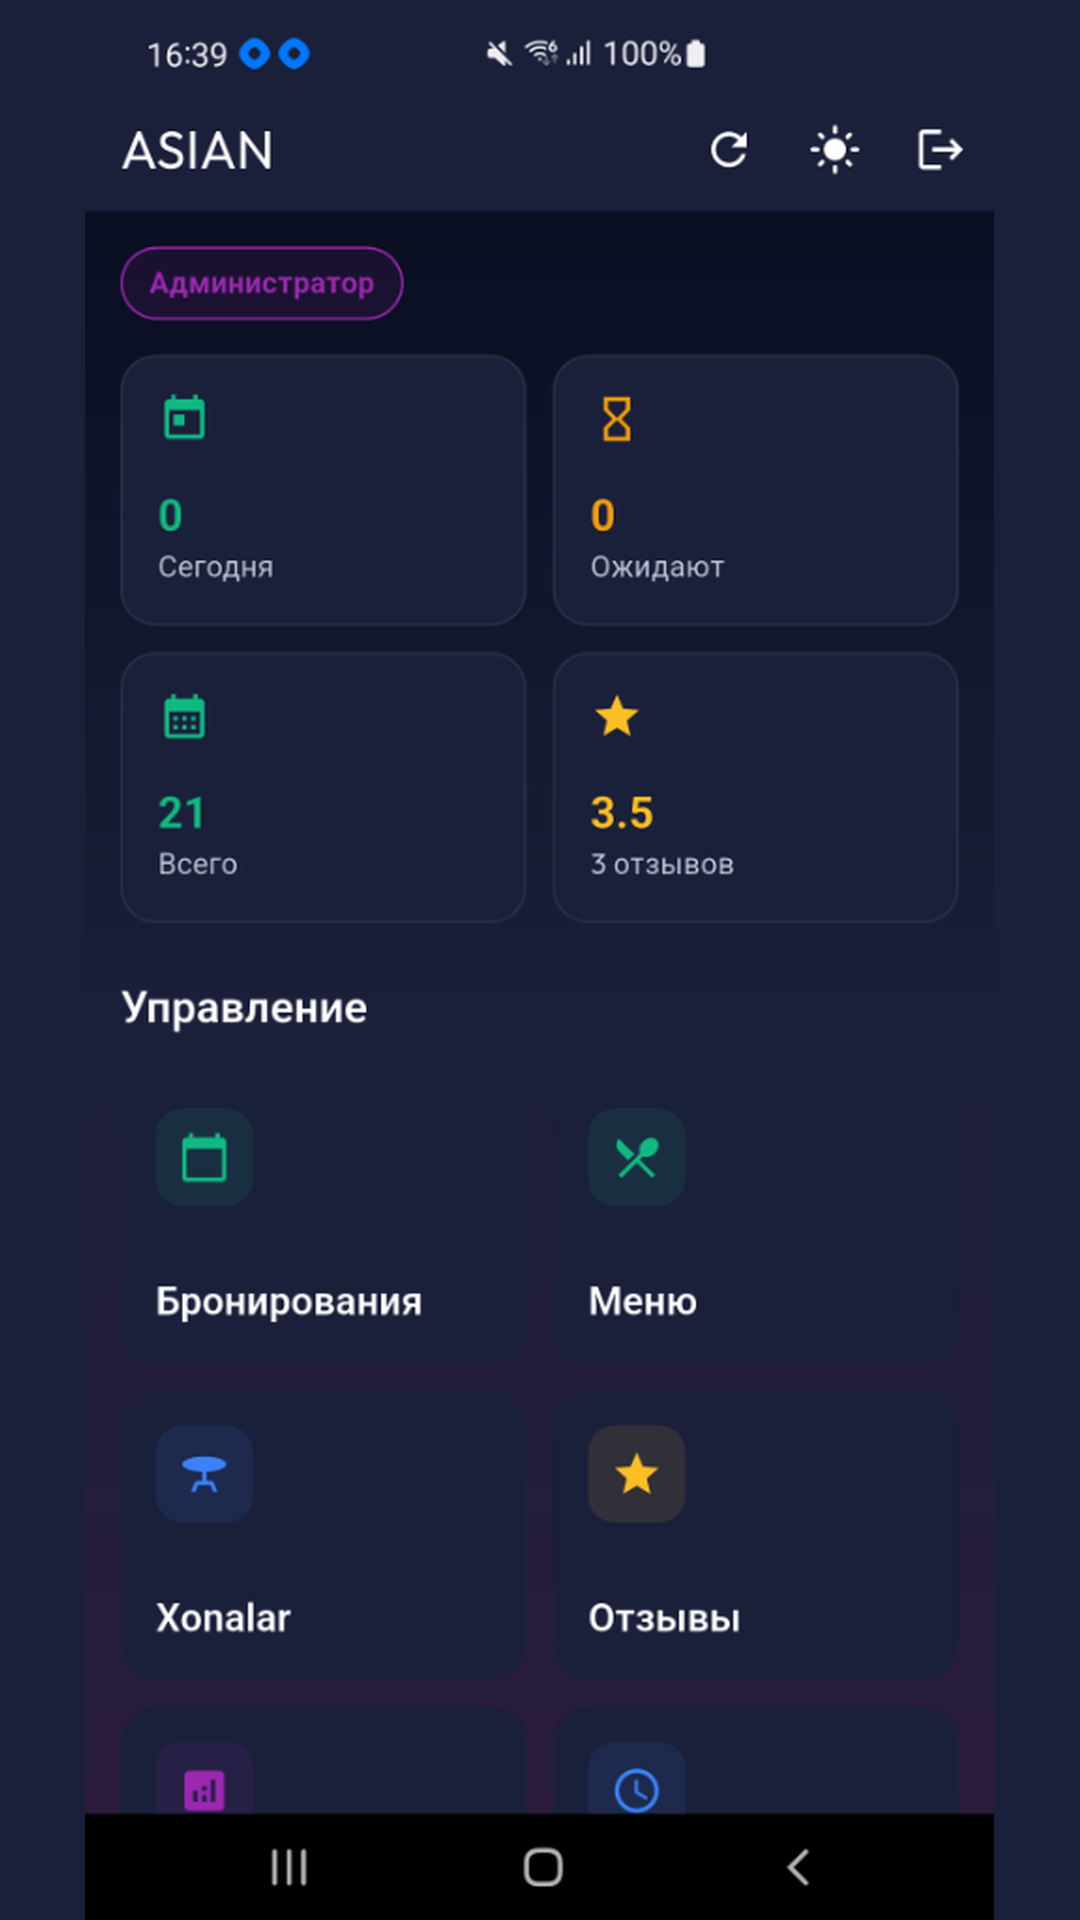
\includegraphics[width=0.4\textwidth]{b_chapters/chapter3/assets/admin_dashboard.png}
  \figsource{CHOYXONA.UZ application screenshot.}
  \caption{Administrator dashboard displaying key performance indicators: today's bookings, pending reservations, total bookings, and average rating.}
  \label{fig:admin-dashboard}
\end{figure}

\subsection{Dashboard and Key Metrics}
\label{subsec:admin-dashboard}

The dashboard home presents key performance indicators (KPIs) at a glance:
\begin{itemize}
  \item \textbf{Today's bookings} --- count with status breakdown (confirmed, pending, checked in, completed);
  \item \textbf{Pending actions} --- items requiring attention (booking confirmations, review responses);
  \item \textbf{Capacity utilization} --- current bookings versus available capacity;
  \item \textbf{Average rating} --- establishment rating with review count;
  \item \textbf{Total bookings} --- cumulative reservation count.
\end{itemize}

Trend indicators compare current values to previous periods (same day last week, monthly averages).
Quick action buttons provide single-tap access to common tasks: view today's schedule, confirm pending bookings, or create a new promotion~\cite{wasserman2010}.

\subsection{Booking and Calendar Management}
\label{subsec:booking-mgmt}

The \textbf{calendar view} provides monthly booking pattern overview with color-coded density cells (light for few, medium for moderate, dark for heavily booked days).
Selecting a day reveals a detailed timeline where bookings appear as positioned blocks with customer name, party size, and room assignment.
Color coding indicates status: blue (confirmed), green (checked in), gray (completed), red (cancelled/no-show).

Booking management capabilities include:
\begin{itemize}
  \item \textbf{Confirmation} --- reviewing and approving new booking requests;
  \item \textbf{Modification} --- adjusting party size, time, or room assignment with audit logging;
  \item \textbf{Cancellation} --- with reason recording and automated customer notification;
  \item \textbf{Check-in/Check-out} --- via QR code scanning or manual search, recording arrival time and actual party size.
\end{itemize}

\subsection{Reports, Analytics, and Menu Management}
\label{subsec:reports-menu}

The \textbf{reports screen} presents analytical views through charts and summary metrics:

\begin{table}[htbp]
\caption{Administrator analytics categories and metrics}
\label{tab:admin-analytics}
\centering
\small
\begin{tabular}{lp{8cm}}
\toprule
\textbf{Category} & \textbf{Metrics} \\
\midrule
Revenue      & Daily totals (line/bar charts), period comparison, estimated from party sizes $\times$ avg.\ check \\
Bookings     & Peak hour distribution, day-of-week patterns, lead time analysis, cancellation rate trends \\
Customers    & New vs.\ returning breakdown, party size distribution, geographic analysis \\
Reviews      & Average rating trend, sentiment indicators, response rate \\
\bottomrule
\end{tabular}
\end{table}

\textbf{Menu management} allows adding items (name, description, price, category, photo), editing, and marking items as temporarily unavailable.
Changes synchronize immediately through Firestore real-time updates.
\textbf{Promotion management} enables creating special offers with title, description, discount details, validity period, and customer targeting~\cite{firebase_firestore2024}.


% =====================================================================
\section{Super Admin Panel and Platform Oversight}
\label{sec:superadmin}

Super administrators oversee the entire CHOYXONA.UZ platform with responsibilities spanning user management, establishment verification, content moderation, and system configuration.
The super admin interface is shown in \cref{fig:superadmin-panel}.

\begin{figure}[htbp]
  \centering
  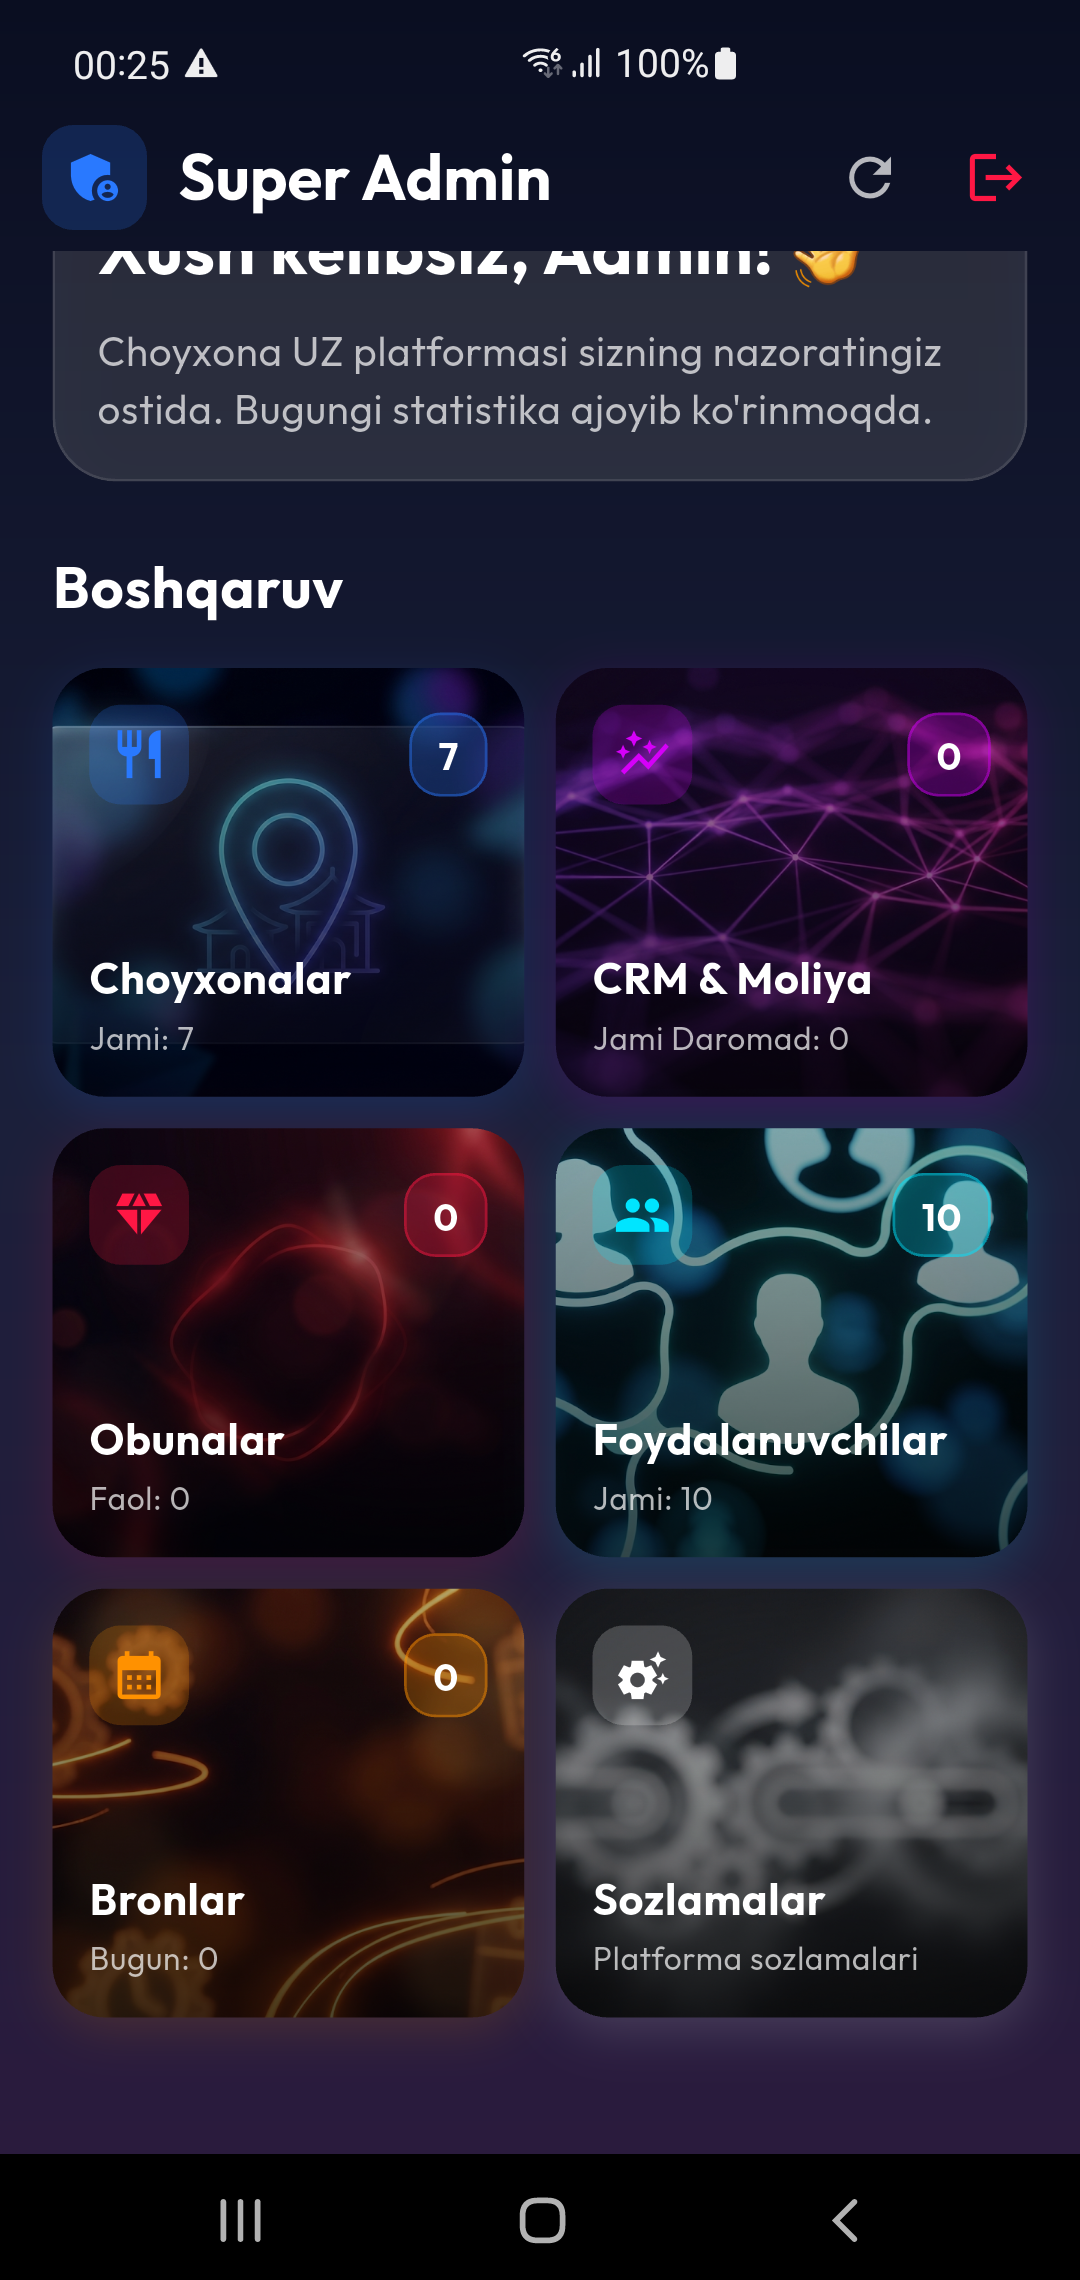
\includegraphics[width=0.4\textwidth]{b_chapters/chapter3/assets/superadmin.png}
  \figsource{CHOYXONA.UZ application screenshot.}
  \caption{Super administrator control panel showing platform-wide management capabilities and monitoring tools.}
  \label{fig:superadmin-panel}
\end{figure}

\subsection{Platform Metrics and Verification}
\label{subsec:platform-metrics}

The super admin dashboard presents platform-wide metrics: total registered users with growth trend, active establishments by region, total processed bookings, and system health indicators.
Growth charts visualize user registration trends, establishment onboarding, and booking volume over time~\cite{jia2014}.

The \textbf{establishment verification workflow} ensures quality of listed businesses:
\begin{enumerate}
  \item New establishments enter \textit{pending} state (invisible to users);
  \item Verification queue shows submitted information and documentation;
  \item Super admin reviews information for completeness and authenticity;
  \item Approval makes establishment visible in search; rejection sends corrective feedback;
  \item Premium verification badges may involve additional steps including in-person visits.
\end{enumerate}

\subsection{User Management and Content Moderation}
\label{subsec:user-management}

User management provides oversight of all registered accounts with search, filtering by role/date/activity, and detailed profile views.
Available moderation actions include:

\begin{itemize}
  \item \textbf{Role modification} --- granting or revoking administrator access;
  \item \textbf{Warning issuance} --- for policy violations (recorded and visible to user);
  \item \textbf{Suspension} --- temporary sign-in prevention during investigations;
  \item \textbf{Permanent ban} --- for severe violations (prevents future registration).
\end{itemize}

Each action logs the super administrator, reason, and timestamp for accountability~\cite{martin2017}.

Content moderation addresses reported reviews through a queue with dismiss/remove/warn options.
Automated keyword filtering flags potentially problematic content for prioritized review.

\subsection{System Configuration}
\label{subsec:system-config}

System configuration enables adjustments without code deployment:
\begin{itemize}
  \item \textbf{Feature flags} --- staged rollout of new functionality to user subsets;
  \item \textbf{Configuration values} --- default search radius, max booking days, min review length;
  \item \textbf{Featured content} --- home screen carousel, promotional banners, announcements.
\end{itemize}

Configurations are stored in a dedicated Firestore collection and loaded by clients during initialization~\cite{firebase_functions2024}.


% =====================================================================
\section{Notification System}
\label{sec:notifications}

The notification system maintains user engagement and delivers timely information throughout the customer journey~\cite{firebase_functions2024}.

Firebase Cloud Messaging (FCM) powers push notifications on both Android and iOS.
The \texttt{PushNotificationService} class manages the complete lifecycle: permission request, device token retrieval and storage, token refresh handling, and notification delivery~\cite{khawas2018}.

Notification categories serve distinct purposes, as summarized in \cref{tab:notification-types}.

\begin{table}[htbp]
\caption{Notification categories, priorities, and trigger conditions}
\label{tab:notification-types}
\centering
\small
\begin{tabular}{llp{5.5cm}}
\toprule
\textbf{Category} & \textbf{Priority} & \textbf{Trigger and Content} \\
\midrule
Booking confirmation & High   & Immediately after reservation: establishment, date, time, reference \\
Reminder (24h)       & Medium & 24 hours before booking \\
Reminder (2h)        & Medium & 2 hours before booking \\
Promotional          & Low    & Special offers from favorited establishments (user-configurable) \\
System               & Low    & Platform announcements, maintenance, new features \\
\bottomrule
\end{tabular}
\end{table}

Notification behavior adapts to application state: \textbf{foreground} notifications display as in-app snackbar overlays; \textbf{background/terminated} notifications appear in the device notification shade and navigate to relevant content on tap.

The notification center (\cref{fig:notifications}) provides persistent history with unread indicators and mark-all-read functionality.

\begin{figure}[htbp]
  \centering
  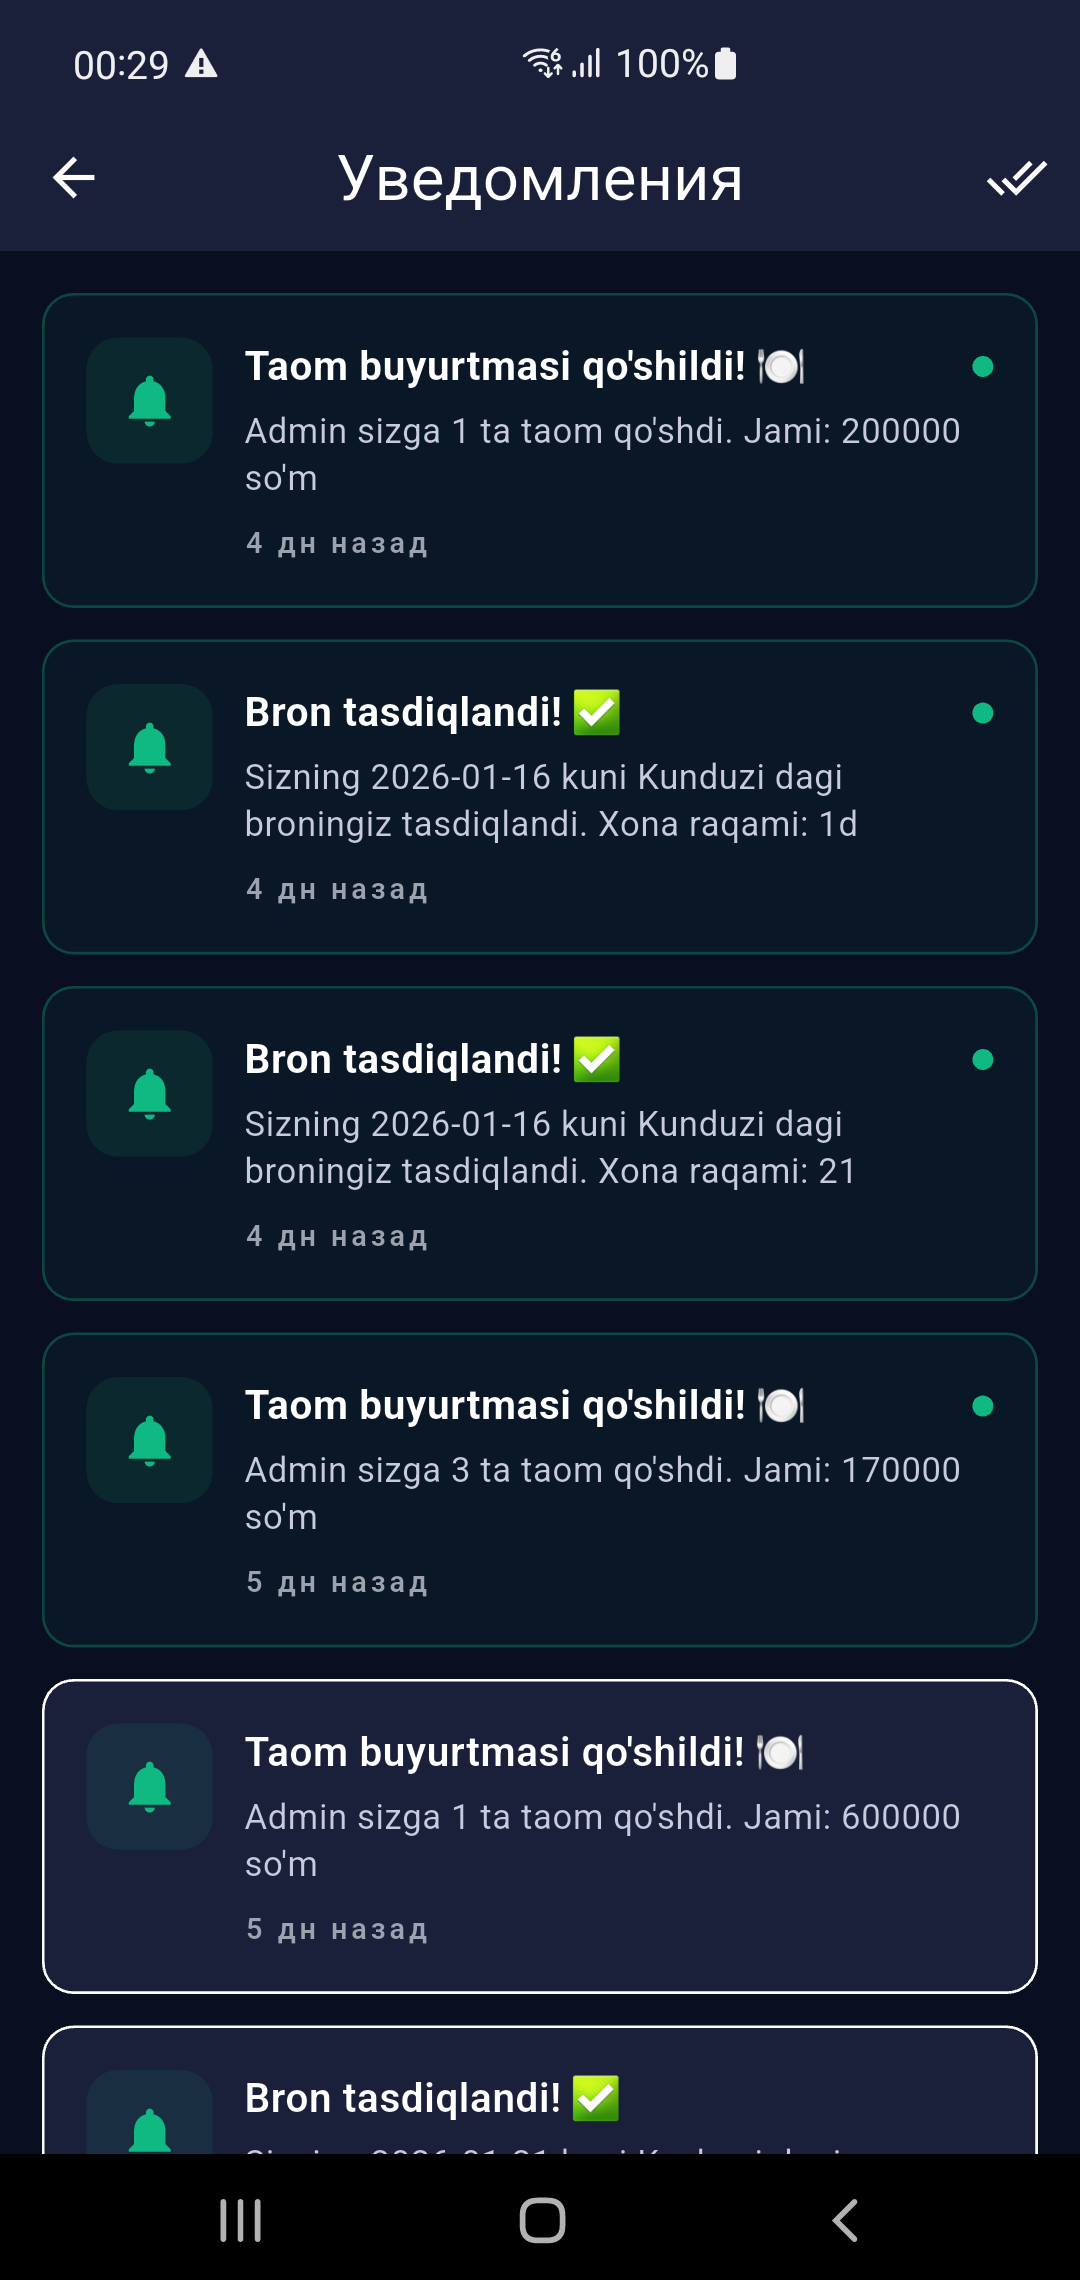
\includegraphics[width=0.4\textwidth]{b_chapters/chapter3/assets/notifications.png}
  \figsource{CHOYXONA.UZ application screenshot.}
  \caption{Notification center displaying booking confirmations, reminders, and system messages with unread indicators.}
  \label{fig:notifications}
\end{figure}

The notification preferences screen provides granular control: independent category toggles and quiet hours configuration.
Preferences update immediately in Firestore~\cite{firebase_firestore2024}.


% =====================================================================
\section{Chapter Summary}
\label{sec:ch3-summary}

This chapter demonstrated the complete functional capabilities of CHOYXONA.UZ through its three user roles:

First, \cref{sec:user-module} described the authentication module supporting email/password and phone/SMS methods (\cref{fig:splash-auth}), role-based access control routing users to appropriate interfaces (\cref{fig:role-routing}), and profile management with cross-device synchronization.

Second, \cref{sec:search-booking} detailed the core customer journey from discovery through booking confirmation.
The multi-dimensional search system (\cref{tab:search-filters}) enables precise establishment matching, while the four-step booking flow (\cref{fig:booking-flow}) guides users through date, time, party, and room selection with transactional consistency ensuring no double-bookings.

Third, \cref{sec:admin-panel} presented the administrator dashboard (\cref{fig:admin-dashboard}) with KPIs, calendar-based booking management, analytics (\cref{tab:admin-analytics}), menu management, and promotion tools.

Fourth, \cref{sec:superadmin} covered the super administrator panel (\cref{fig:superadmin-panel}) providing platform oversight through establishment verification workflows, user management with moderation actions, content moderation, and remote system configuration.

Fifth, \cref{sec:notifications} described the FCM-based notification system with five categories (\cref{tab:notification-types}), adaptive behavior based on application state, and user-configurable preferences.

These functional capabilities collectively deliver a comprehensive three-sided marketplace connecting customers, establishment administrators, and platform operators.
The testing and deployment of this implementation are addressed in Chapter~4.

\chapter{Testing, Deployment, and Future Development}
\label{ch:testing}

% PLACEHOLDER - will be written after Chapter 3 is approved
\textit{This chapter will be written after Chapter~3 review is completed.}


% ===== Conclusions =====
\unchapter{Conclusions}

% PLACEHOLDER - will be written at the end
\textit{Conclusions will be written after all chapters are completed.}


% ===== Literature =====
\printbibliography[heading=bibintoc,title=Literature]


% ===== Appendices =====
\appendix
\chapter{Application Screenshots}
\label{app:screenshots}

This appendix presents selected screenshots from the CHOYXONA.UZ application demonstrating the user interface across different user roles and key workflows.

\begin{figure}[htbp]
  \centering
  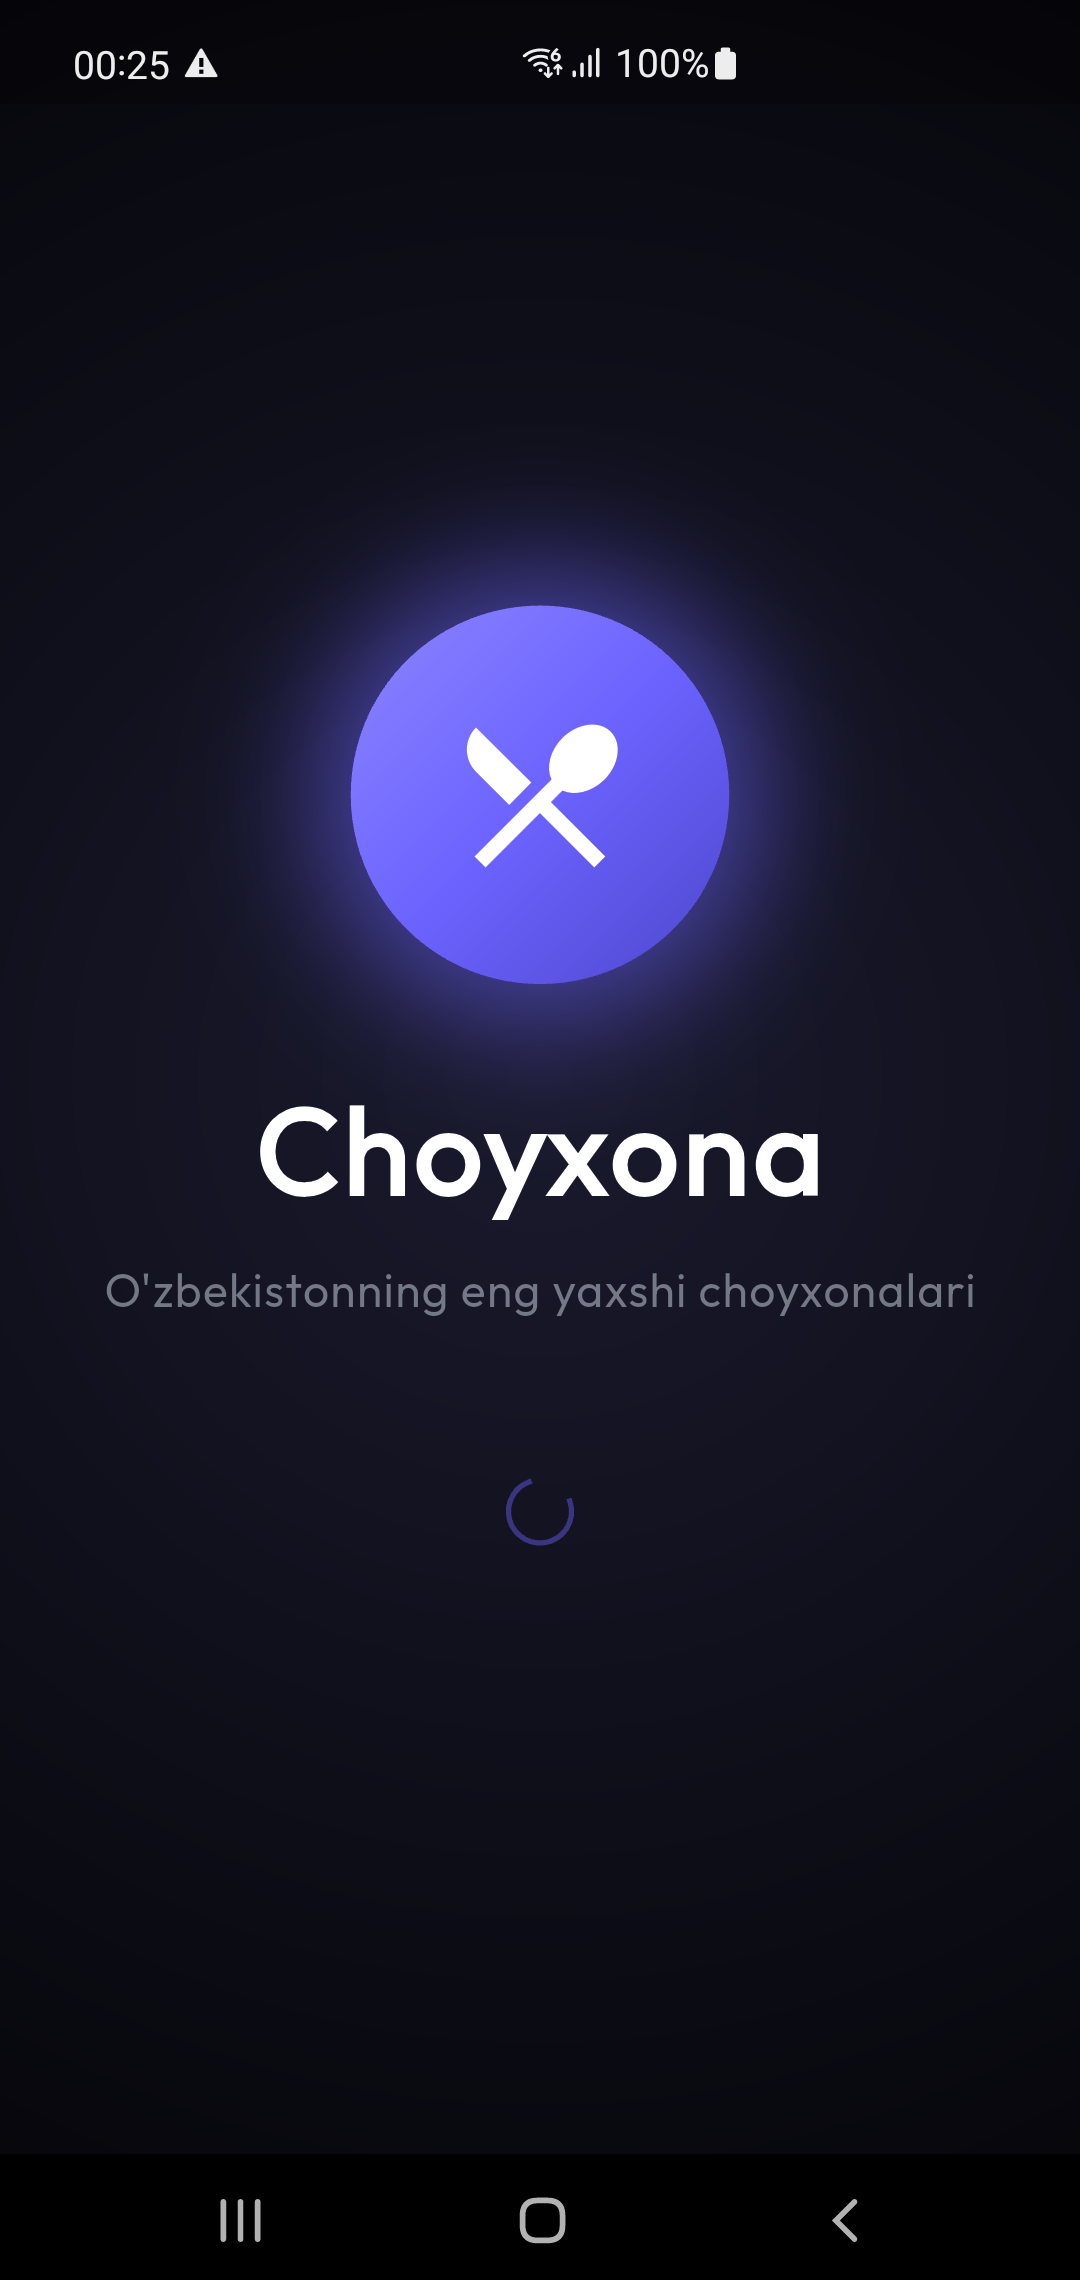
\includegraphics[width=0.35\textwidth]{b_chapters/chapter3/assets/splash_screen.png}
  \caption{CHOYXONA.UZ splash screen displayed during application initialization.}
  \label{fig:app-splash}
\end{figure}

\begin{figure}[htbp]
  \centering
  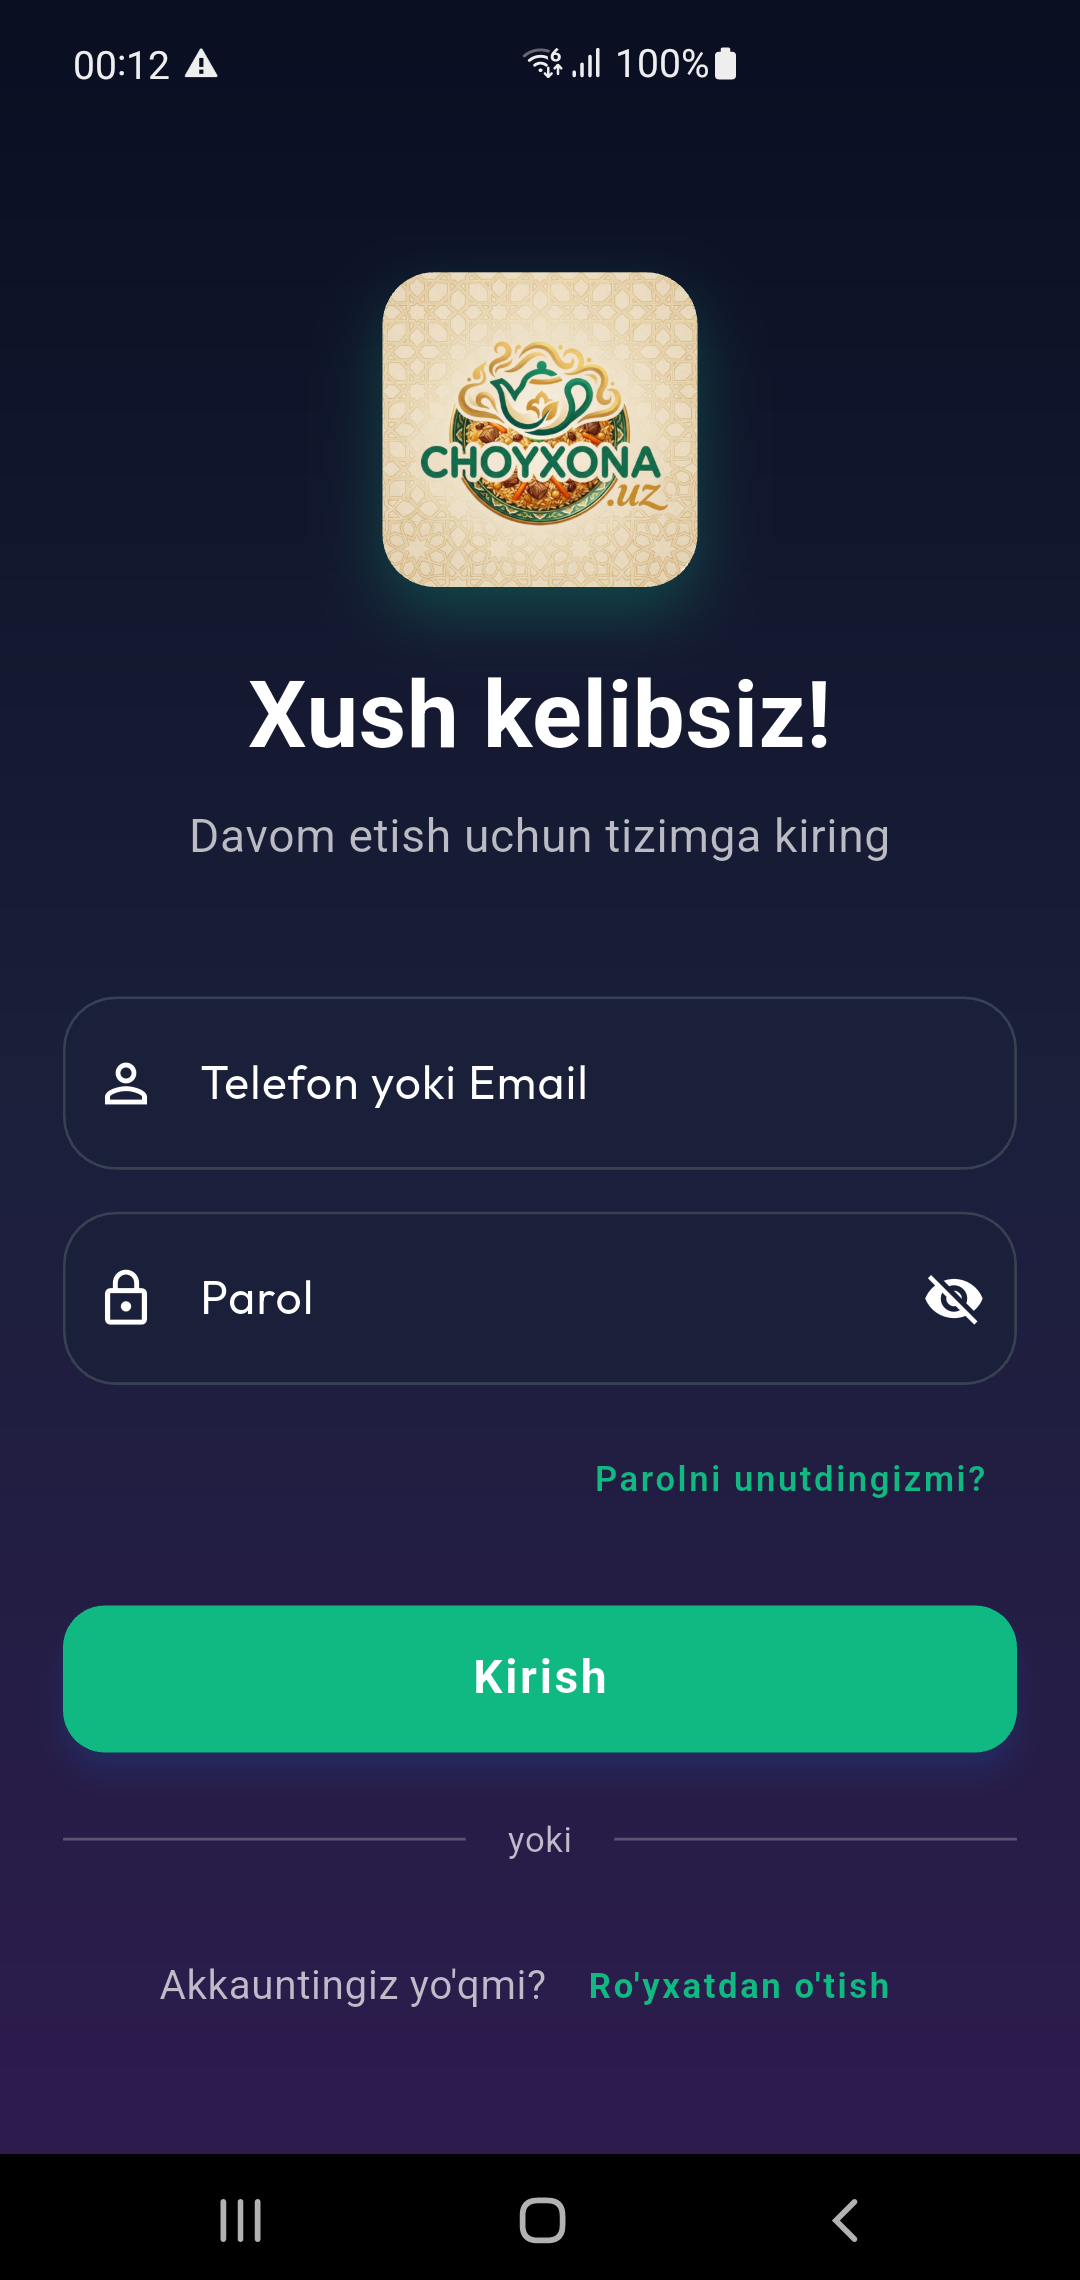
\includegraphics[width=0.35\textwidth]{b_chapters/chapter3/assets/auth_screen.png}
  \caption{Authentication screen with email/phone and password input fields.}
  \label{fig:app-auth}
\end{figure}

\begin{figure}[htbp]
  \centering
  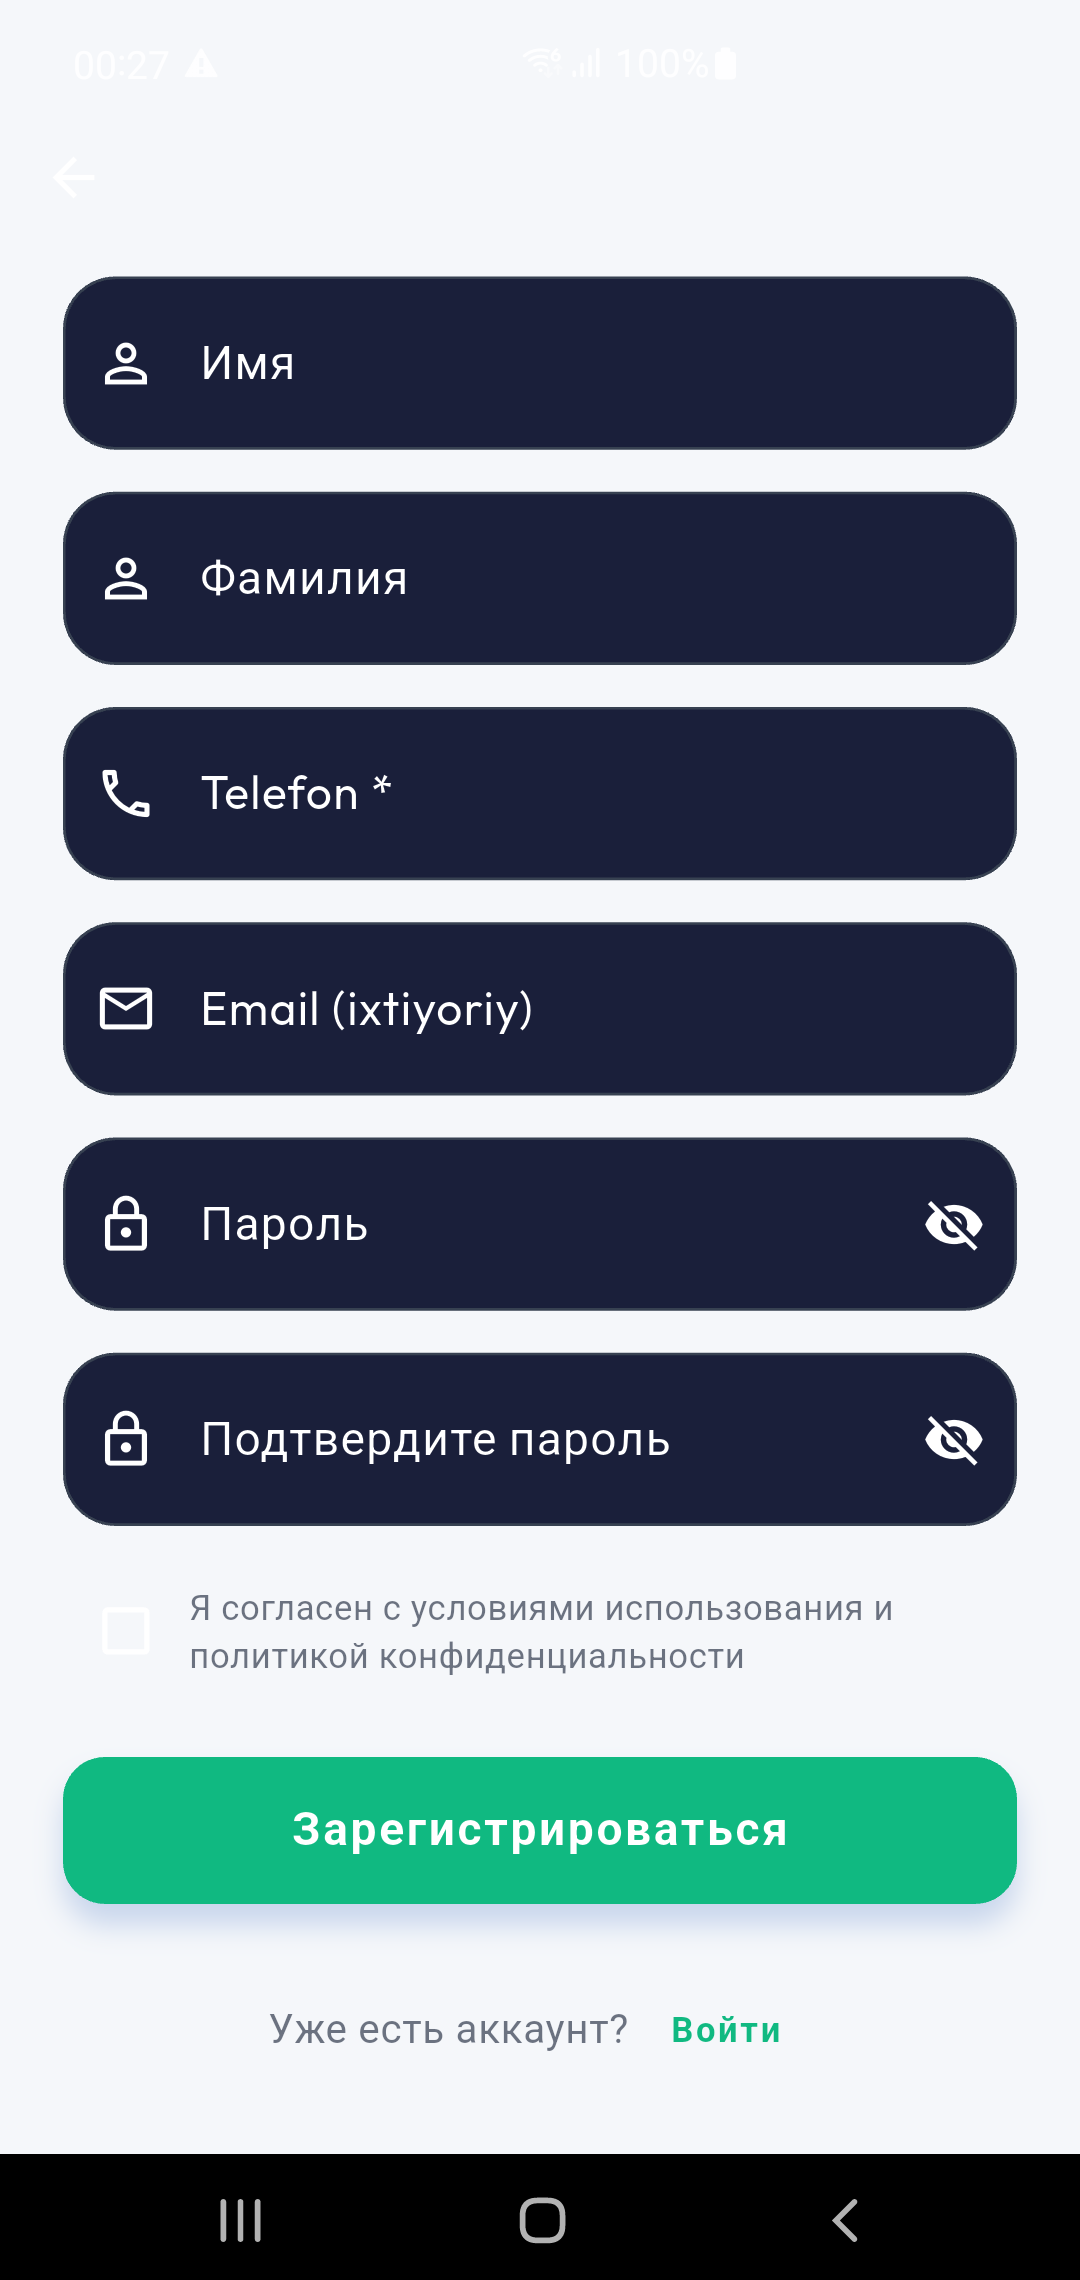
\includegraphics[width=0.35\textwidth]{b_chapters/chapter3/assets/regist_screen.png}
  \caption{User registration screen for new account creation.}
  \label{fig:app-register}
\end{figure}

\begin{figure}[htbp]
  \centering
  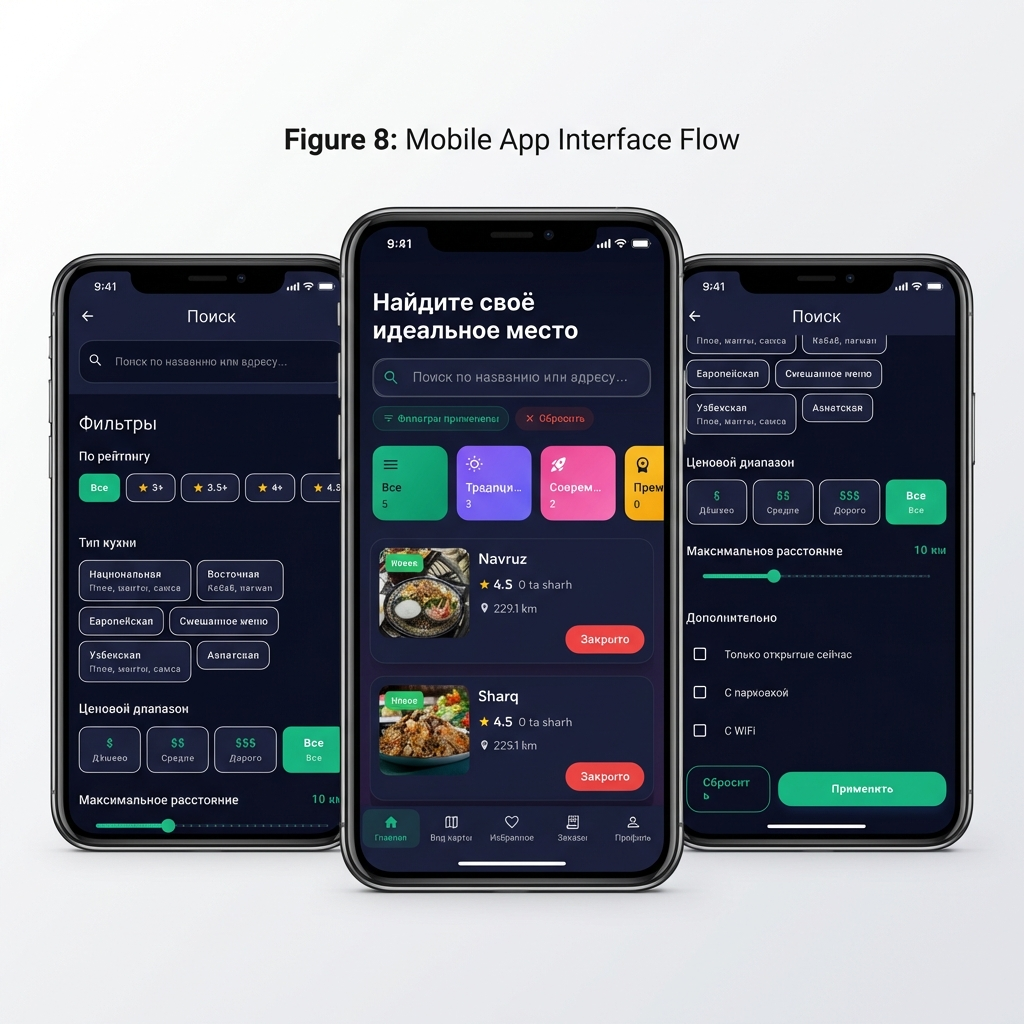
\includegraphics[width=0.7\textwidth]{b_chapters/chapter3/assets/user_collage.png}
  \caption{Customer-facing interface: home screen, establishment details, and booking views.}
  \label{fig:app-user-collage}
\end{figure}

\begin{figure}[htbp]
  \centering
  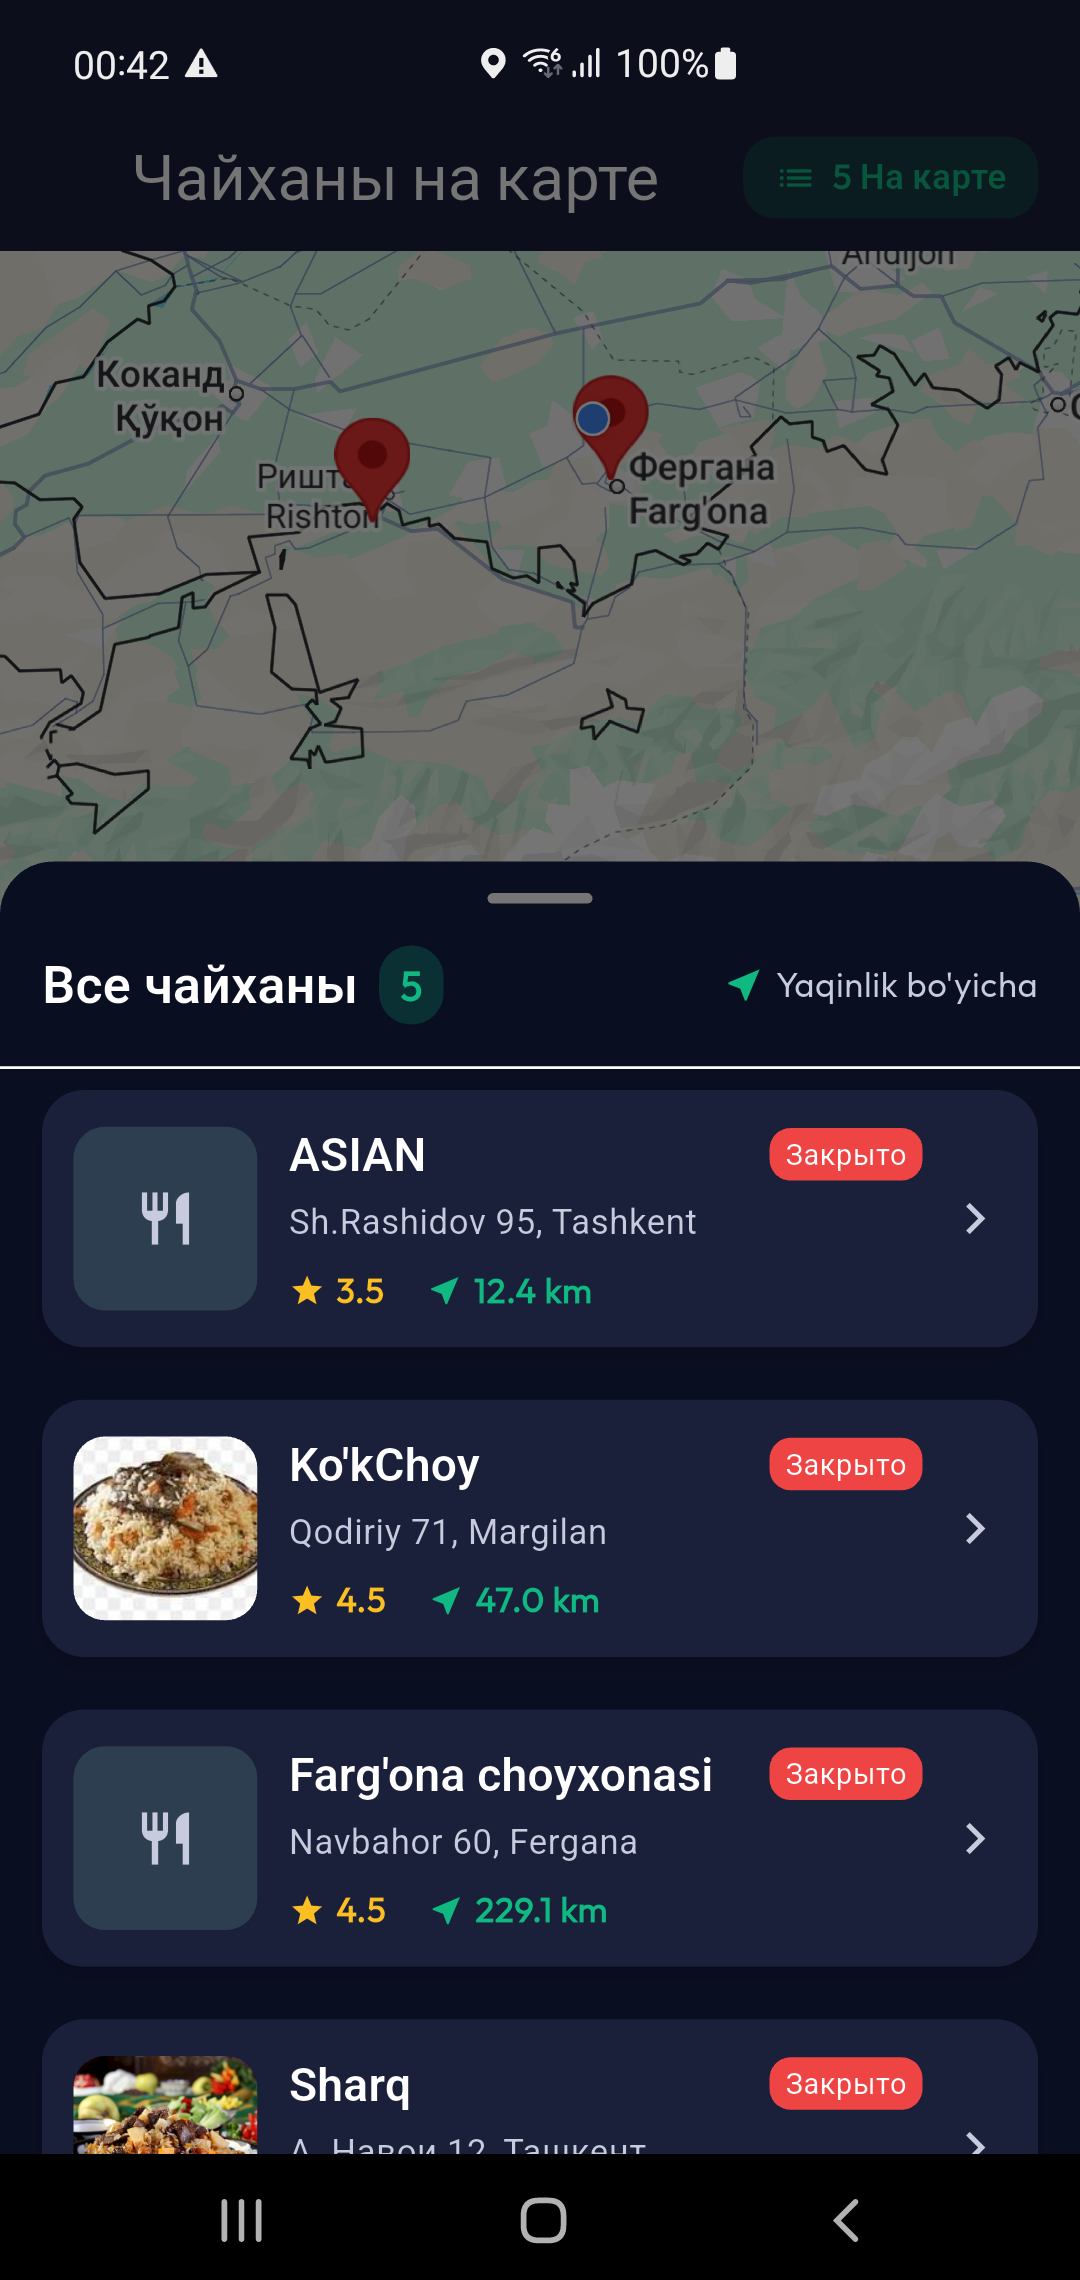
\includegraphics[width=0.7\textwidth]{b_chapters/chapter2/assets/google_maps.png}
  \caption{Google Maps integration showing establishment locations with interactive markers.}
  \label{fig:app-maps}
\end{figure}

\begin{figure}[htbp]
  \centering
  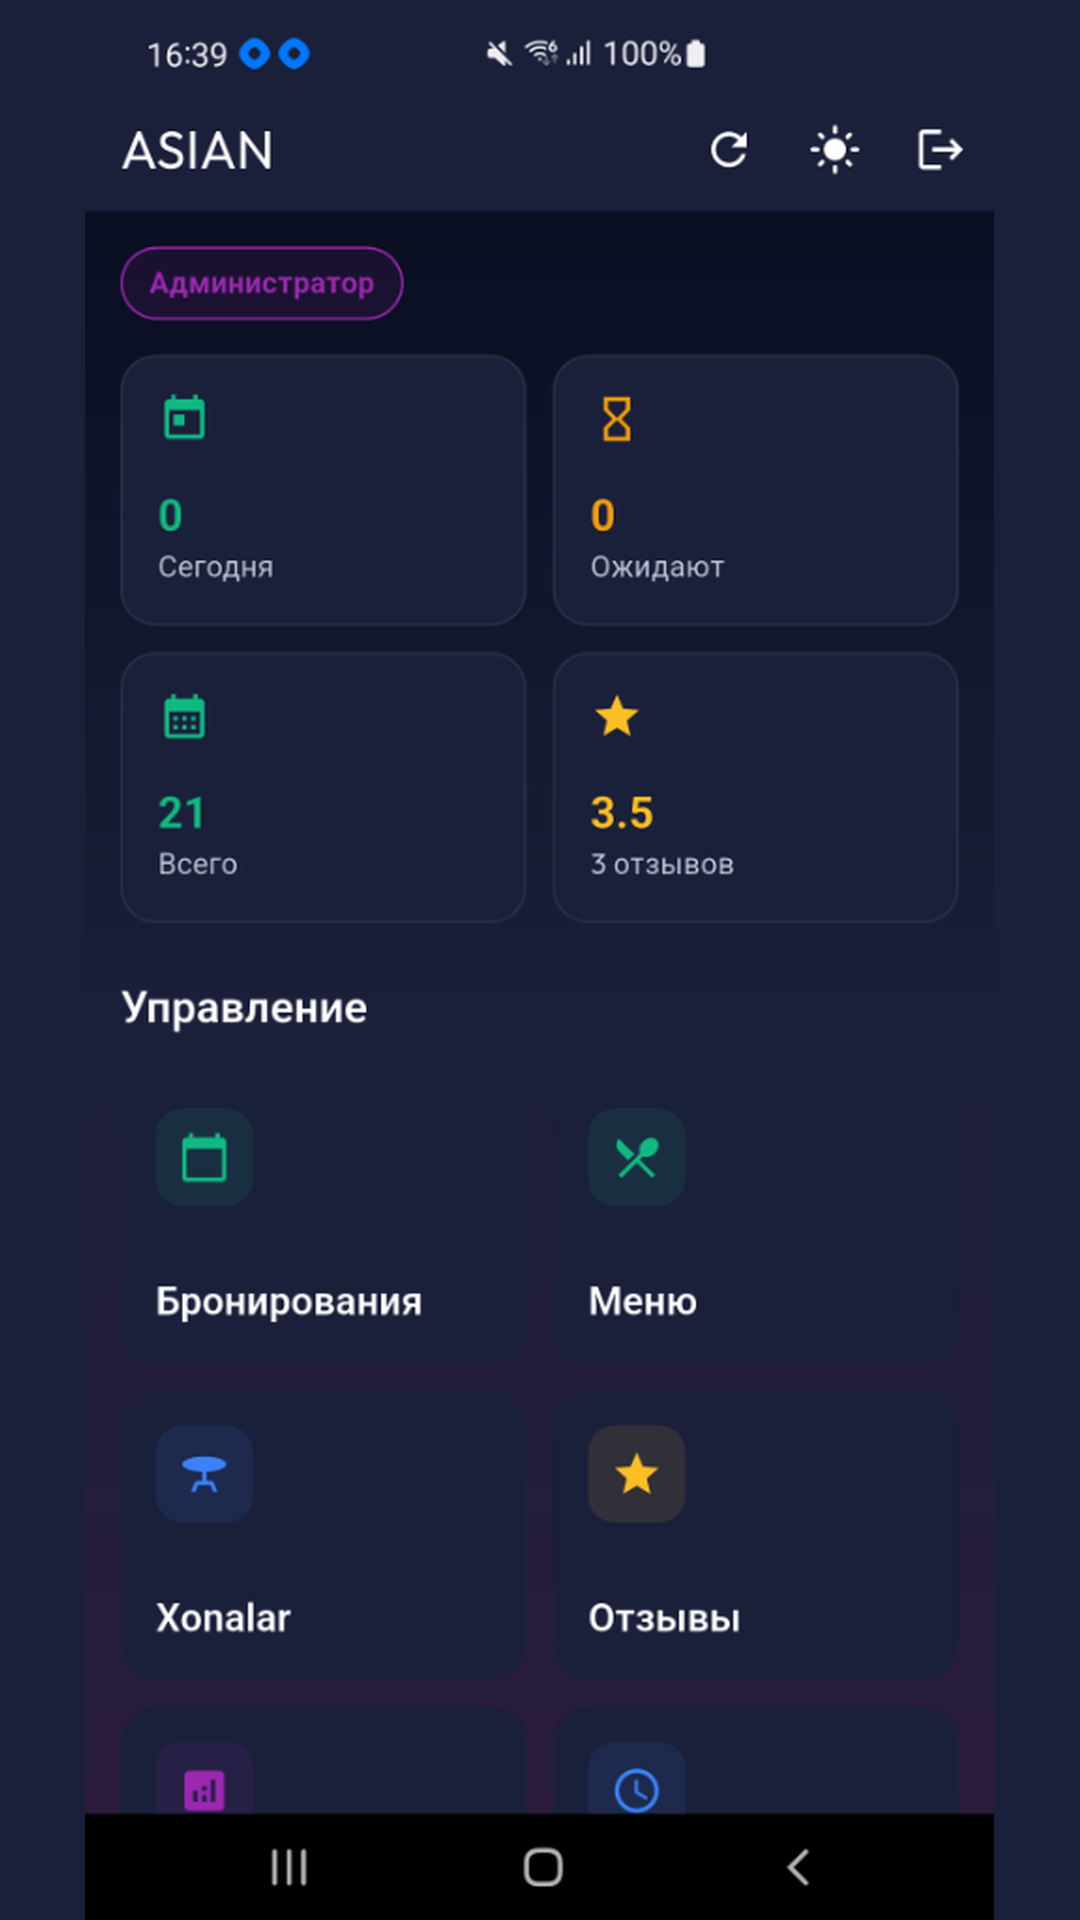
\includegraphics[width=0.35\textwidth]{b_chapters/chapter3/assets/admin_dashboard.png}
  \caption{Administrator dashboard with key performance indicators and management tools.}
  \label{fig:app-admin}
\end{figure}

\begin{figure}[htbp]
  \centering
  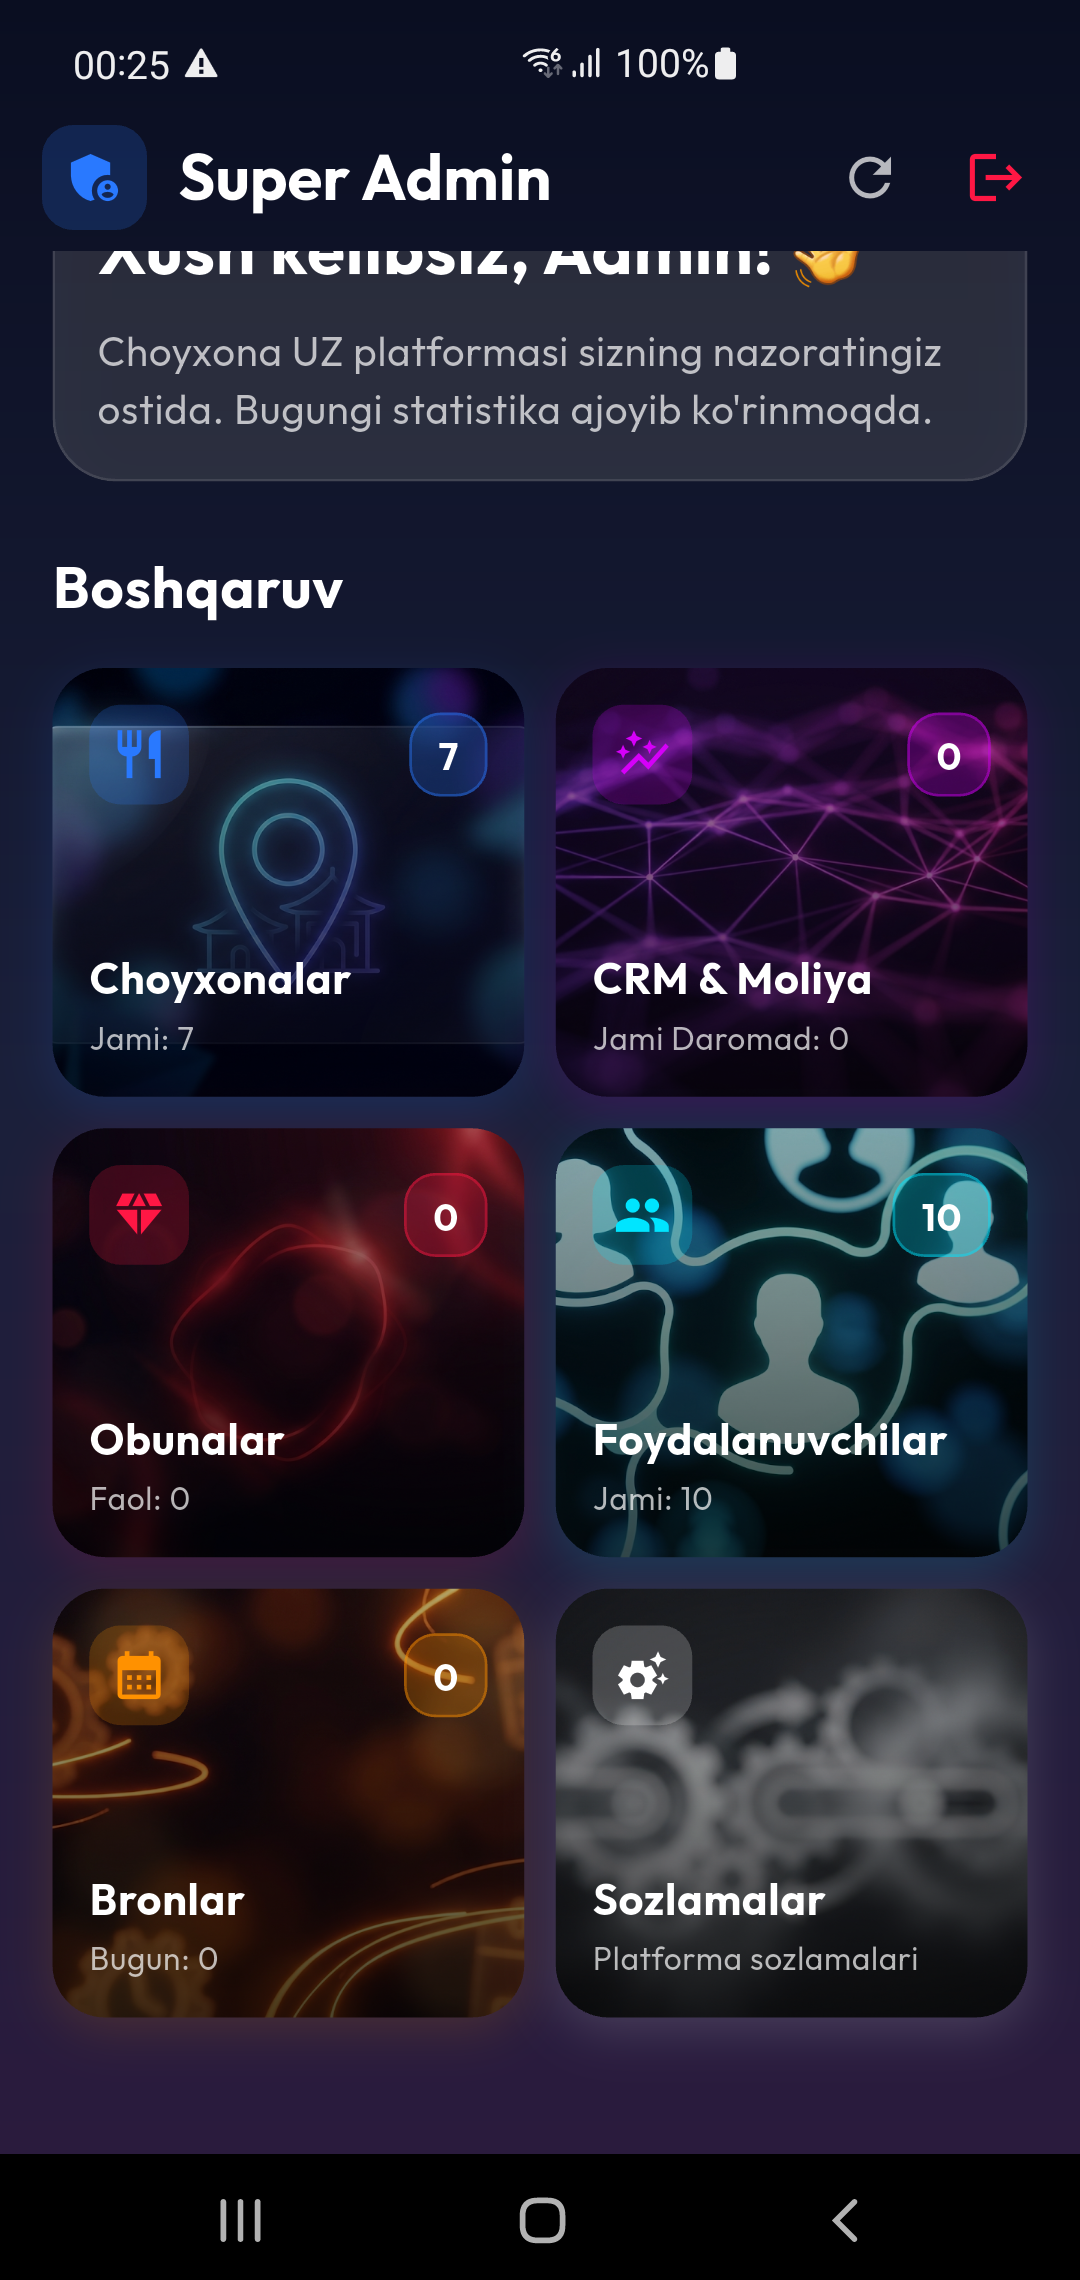
\includegraphics[width=0.7\textwidth]{b_chapters/chapter3/assets/superadmin.png}
  \caption{Super administrator control panel for platform-wide management and monitoring.}
  \label{fig:app-superadmin}
\end{figure}

\chapter{Expert Evaluation Criteria for Final Thesis Quality}
\label{app:evaluation}

\begin{table}[htbp]
\caption{Expert evaluation criteria for the quality of the final thesis}
\label{tab:eval-criteria}
\centering
\small
\begin{tabular}{clc}
\toprule
\textbf{No.} & \textbf{Criterion title and content} & \textbf{Points} \\
\midrule
1 & Conformity of the thesis title to the research area; style; correctness of key words. & 5 \\
2 & Thesis structure: presence of the essential chapters. & 5 \\
3 & Level of research motivation grounded in the contemporary state of the problem. & 5 \\
4 & Quality and correctness of the theses to be defended; novelty of the main results. & 5 \\
5 & Adequacy of the research methodology to the formulated research problem. & 5 \\
6 & Originality of the research problem. & 5 \\
7 & Use of constructive methods (incl.\ mathematical and computational) in solving the research problems. & 5 \\
8 & Quality of conclusions: justification and correctness. & 5 \\
9 & Quality of thesis formatting, literary style, compliance with standards and regulations. & 5 \\
10 & Quality of the list of references: currency, authority, presence of sources in foreign languages. & 5 \\
\midrule
 & \textbf{Total} & \textbf{50} \\
\bottomrule
\end{tabular}
\end{table}

\textbf{Note:}
\begin{enumerate}
  \item All criteria are mandatory.
  \item Final thesis evaluation:
  \begin{itemize}
    \item $<25$ points --- the thesis does not meet the requirements;
    \item 25--35 points --- the thesis requires improvement;
    \item 36--50 points --- the thesis is eligible for defense.
  \end{itemize}
\end{enumerate}

% ===== Declarations & Acknowledgments =====
\frontmatterpage
\unchapter{Affirmation}

\textit{Hereby I, \studentnameEN, affirm that the Bachelor's thesis was performed independently, without the assistance of others; sources of data and definitions used in the work are indicated. This work has not been submitted to any other examination commission and has not been published elsewhere.}

\vspace{14mm}
\noindent Riga, 20\underline{\hspace{1cm}}.\ \underline{\hspace{2.5cm}}.\hspace{1cm}\rule{5cm}{0.4pt}\\
\hspace*{7.1cm}\scriptsize signature, full name \hfill

\frontmatterpage
\unchapter{Acknowledgments}

The author expresses sincere gratitude to the thesis supervisor, Professor Jelena Caiko, for her guidance, expert advice, and continuous support throughout the research and development process.
Her feedback significantly improved both the practical implementation and the academic presentation of this work.

Special thanks are extended to the beta testers who invested their time to evaluate early versions of the CHOYXONA.UZ application, report issues, and provide constructive suggestions that shaped the final product.

The author is grateful to the restaurant and teahouse owners in Uzbekistan who participated in the project by registering their establishments on the platform and providing valuable feedback on the administrator interface from a real business operations perspective.

Finally, appreciation extends to the open-source communities maintaining Flutter, Firebase, and the numerous packages that accelerated development.
Their collective contributions to the software ecosystem make projects like this possible.

\end{document}
